% ============================================================
%  MSc Project Report
%  Topic : Causal Inference for Robotic Grasp Failure
%           Diagnosis under Perceptual Degradation
%           (MuJoCo + Contact-GraspNet)
%
%  Student : Bonolo Masima (3175764M)
%  Programme: MSc Robotics and AI
%  University: University of Glasgow
%  School  : James Watt School of Engineering
%  Supervisor: Dr Dezong Zhao
%  Date    : \today
% ============================================================

\documentclass[11pt,a4paper]{report}

% ── Page geometry ────────────────────────────────────────────
\usepackage[
  top=25mm,
  bottom=25mm,
  left=32mm,
  right=26mm,
  headheight=14pt
]{geometry}

% ── Packages ────────────────────────────────────────────────
\usepackage[T1]{fontenc}
\usepackage[utf8]{inputenc}
% Times-based text and math fonts (matches the reference paper style)
\usepackage{newtxtext}
\usepackage{newtxmath}
\usepackage{setspace}
\setstretch{1.1}

% ── Paragraph style (indented, no inter-paragraph gap) ───────
\setlength{\parindent}{1.5em}
\setlength{\parskip}{0pt plus 1pt}

\usepackage{amsmath,amssymb,amsthm}
\usepackage{bm}
\usepackage{graphicx}
\usepackage{booktabs}
\usepackage{multirow}
\usepackage{array}
\usepackage{longtable}
\usepackage{xcolor}
\usepackage{algorithm}
\usepackage{algpseudocode}
\usepackage{tikz}
\usetikzlibrary{arrows.meta,positioning,fit,backgrounds}
\usepackage{pgfplots}
\pgfplotsset{compat=1.18}
\usepackage{subcaption}
\usepackage{listings}
\usepackage{url}
\usepackage{hyperref}
\hypersetup{
  colorlinks = true,
  linkcolor  = blue!70!black,
  citecolor  = teal,
  urlcolor   = blue!70!black
}
\usepackage{fancyhdr}
\usepackage{titlesec}

% ── Section heading style (matches reference paper: bold, compact) ─
\titleformat{\chapter}[hang]
  {\normalfont\large\bfseries}{\thechapter}{1em}{}
\titlespacing*{\chapter}{0pt}{24pt}{10pt}

\titleformat{\section}[hang]
  {\normalfont\normalsize\bfseries}{\thesection}{1em}{}
\titlespacing*{\section}{0pt}{14pt}{4pt}

\titleformat{\subsection}[hang]
  {\normalfont\normalsize\itshape\bfseries}{\thesubsection}{1em}{}
\titlespacing*{\subsection}{0pt}{10pt}{3pt}

\titleformat{\subsubsection}[runin]
  {\normalfont\normalsize\bfseries}{\thesubsubsection}{1em}{}[.]
\titlespacing*{\subsubsection}{0pt}{8pt}{6pt}

\usepackage{caption}

% ── Caption style (smaller font, "Figure X:" label) ──────────
\captionsetup{
  font=small,
  labelfont=normalfont,
  labelsep=colon,
  justification=justified,
  singlelinecheck=false
}

% ── Code listings style ─────────────────────────────────────
\lstset{
  language=Python,
  basicstyle=\ttfamily\small,
  keywordstyle=\color{blue!70!black}\bfseries,
  commentstyle=\color{green!50!black}\itshape,
  stringstyle=\color{red!60!black},
  numbers=left,
  numberstyle=\tiny\color{gray},
  numbersep=8pt,
  frame=single,
  framesep=4pt,
  breaklines=true,
  showstringspaces=false,
  tabsize=4,
  captionpos=b,
  xleftmargin=15pt,
  xrightmargin=5pt
}

\lstdefinestyle{xml}{
  language=XML,
  basicstyle=\ttfamily\small,
  keywordstyle=\color{blue!70!black},
  commentstyle=\color{green!50!black}\itshape,
  stringstyle=\color{red!60!black},
  numbers=left,
  numberstyle=\tiny\color{gray},
  frame=single,
  breaklines=true,
  showstringspaces=false,
  tabsize=2,
  captionpos=b,
  xleftmargin=15pt,
  morekeywords={mujoco,compiler,option,default,geom,worldbody,body,
                joint,inertial,site,camera,tendon,fixed,equality,
                actuator,general,keyframe,key,light,freejoint}
}

% ── Headers and footers ─────────────────────────────────────
\pagestyle{fancy}
\fancyhf{}
\fancyhead[L]{\leftmark}
\fancyhead[R]{Bonolo Masima --- 3175764M}
\fancyfoot[C]{\thepage}
\renewcommand{\headrulewidth}{0.4pt}

% ── Theorem environments ────────────────────────────────────
\newtheorem{definition}{Definition}[chapter]
\newtheorem{proposition}{Proposition}[chapter]
\newtheorem{hypothesis}{Hypothesis}[chapter]

% ── Custom commands ─────────────────────────────────────────
\newcommand{\doop}{\operatorname{do}}
\newcommand{\SCM}{\mathcal{M}}
\newcommand{\EE}{\mathbb{E}}
\newcommand{\RR}{\mathbb{R}}

% ============================================================
%  TITLE PAGE
% ============================================================
\begin{document}

\begin{titlepage}
  \centering
  \vspace*{1cm}

  {\Large\textbf{University of Glasgow}}\\[0.3cm]
  {\large James Watt School of Engineering}\\[0.3cm]
  {\large MSc Robotics and AI}\\[2cm]

  {\LARGE\textbf{Causal Inference for Robotic Grasp Failure\\
  Diagnosis under Perceptual Degradation}}\\[2cm]

  {\Large Bonolo Masima}\\[0.3cm]
  {\large Student Number: 3175764M}\\[2cm]

  \textbf{Supervisor:} Dr Dezong Zhao\\[0.5cm]
  \textbf{Second Marker:} [To be assigned]\\[2cm]

  Submitted in partial fulfilment of the requirements for the degree of\\
  \textbf{Master of Science in Robotics and AI}\\[1cm]

  \vfill
  {\large \today}
\end{titlepage}

% ============================================================
%  DECLARATION
% ============================================================
\chapter*{Declaration}
\addcontentsline{toc}{chapter}{Declaration}

I declare that this thesis has been composed solely by myself and that it has not been submitted, in whole or in part, in any previous application for a degree. Except where stated otherwise by reference or acknowledgement, the work presented is entirely my own.

\vspace{2cm}
\noindent
\textbf{Bonolo Masima}\\
\today

% ============================================================
%  ABSTRACT
% ============================================================
\chapter*{Abstract}
\addcontentsline{toc}{chapter}{Abstract}

This thesis develops and audits a pre-registered and revised mechanistic Structural Causal Model (SCM) for diagnosing robotic grasp failure. Given a failed grasp attempt, we ask whether Pearl's three-step counterfactual procedure---abduction, action, and prediction---applied to an SCM derived from the known dataflow of the perception-action pipeline, can correctly attribute the failure to its environmental root cause when a single cause exists, and correctly recognise the failure as irreducibly multi-causal when it does not. Because the perturbations are experimenter-controlled, the true cause of each failure is always available for scoring against simulated ground truth, making this a falsifiable methodological audit rather than an unfalsifiable post-hoc narrative. As a secondary comparison, we contrast this structured diagnosis against a zero-shot vision-language model~(LLM) (a VLM-capable model given text only, not images) given identical observational data, to quantify what the SCM's explicit structural knowledge of the pipeline contributes relative to associative natural-language reasoning.

The SCM links four independently controllable perceptual variables---depth noise~($\sigma_d$), point cloud sparsity~($\rho$), viewpoint elevation~($\phi$), and viewpoint azimuth~($\theta$)---through measurable intermediate variables (point cloud completeness, the number of grasp candidates, grasp confidence, and pose error) to binary grasp success. The approach is implemented in MuJoCo with Contact-GraspNet as the grasp synthesis model, injecting synthetic Gaussian depth noise directly onto the simulated depth buffer to obtain perturbations that are causally clean and independently controlled, a level of experimental precision that is difficult to achieve on physical hardware. The confirmatory study is a 7{,}560-trial floating-gripper factorial grid with a physical hold/lift outcome. Unfiltered top-1 execution succeeds in 5.0\% of trials; 72.8\% fail at an open-hand pre-grasp collision before lift is attempted. Depth noise moves that collision gate and post-gate hold in opposite directions, so the marginal success rate is not monotone, and object geometry dominates execution. A targeted top-$k$ collision filter at one clean viewpoint reaches 89\% under a lighter clamp-and-lift criterion, showing that the 5.0\% headline is mostly pose selection rather than a gripper that cannot lift. A 432-trial proximity study---grasp success falling from 70.4\% under a noise-free sensor to 0.0\% under the most severe noise---was the pilot that motivated this redesign. The SCM-versus-LLM comparison is scored on that pilot outcome (attribution accuracy, consistency, explanation quality) and is not re-scored on physical grasps.

\textbf{Keywords:} Causal Inference, Counterfactual Reasoning, Grasp Failure Diagnosis, Structural Causal Model, Point Cloud, MuJoCo, Contact-GraspNet, Large Language Models, Perceptual Degradation.

% ============================================================
%  ACKNOWLEDGEMENTS
% ============================================================
\chapter*{Acknowledgements}
\addcontentsline{toc}{chapter}{Acknowledgements}

I would like to express my sincere gratitude to my supervisor, Dr Dezong Zhao, for his guidance, patience, and invaluable feedback throughout this project. His expertise in robotics and causal reasoning has been instrumental in shaping the direction of this work.

I also wish to thank the James Watt School of Engineering at the University of Glasgow for providing the computational resources and academic environment necessary to complete this project.

Finally, I am grateful to my family and friends for their unwavering support and encouragement throughout my studies.

% ============================================================
%  TABLE OF CONTENTS, LIST OF FIGURES, LIST OF TABLES
% ============================================================
\tableofcontents
\listoffigures
\listoftables

% ============================================================
%  CHAPTER 1: INTRODUCTION
% ============================================================
\chapter{Introduction}
\label{ch:intro}

\section{Motivation and Context}
\label{sec:motivation}

Data-driven grasp synthesis algorithms often achieve high success rates under laboratory conditions. For example, Contact-GraspNet (CGN)~\cite{sundermeyer2021contact} achieves over 90\% grasp success on unseen objects in structured clutter. However, these figures are achieved under controlled conditions, including a collision-aware selection stage that filters candidate grasps before execution, a well-calibrated environment, a favourable camera viewpoint and a specified gripper. Achieving such high grasp success rates requires great engineering effort, as we demonstrate in Appendix~\ref{app:implementation}.

\noindent When deployed in the real world, these high grasp success rates often fail to transfer. This results from combined effects of perception (depth sensor noise), geometry (unfavourable viewpoints causing partial observability) and physics (pre-grasp collisions, friction, mass effects). Determining which effect is responsible for a given failure is hard. As a result, success or failure of a grasp cannot be attributed back to its contributing causes. For example, is a failed grasp caused by a noisy depth image, a setup that leaves the camera and gripper poorly positioned or a collision during execution? Contact-GraspNet's black-box nature compounds this problem, since its internal reasoning cannot be inspected. Even a fully transparent version of the algorithm would not reveal which layer was at fault in a given trial. Therefore, when a grasp fails the system only knows that it failed, not why.

\noindent Tracing a failure back to its cause requires an explicit model of how the stages of the pipeline causally depend on one another, i.e. a structural model. Trustworthy autonomy demands that we know \emph{why} a trusted algorithm fails. This thesis argues that we must make the preconditions of success explicit and measure how much each one contributes to failure. Doing so requires a causal audit of the perception-action pipeline.

\section{The Diagnostic Gap}
\label{sec:diagnostic_gap}

Existing approaches to handling grasp failure include retry policies, anomaly detection, reinforcement learning, statistical causal discovery, learned causal explanation and vision language models. Each addresses part of the diagnostic problem, but falls short of a full structural account. Retry policies re-attempt a failed grasp under stochastic variation but do not identify which precondition of success was violated. Anomaly detection flags that a trial is unusual relative to a learned distribution but does not attribute the anomaly to a specific mechanistic cause.

\noindent
\begin{minipage}[t]{0.40\textwidth}
  \vspace{0pt}
  Reinforcement learning methods optimise policies to avoid failure modes empirically, without producing an explicit causal model of why any single trial failed. Statistical causal discovery learns a graph structure from observational data, but the graph it recovers is only as reliable as the independence assumptions and sample sizes available, and it is not grounded in the pipeline's known architecture.
\end{minipage}\hfill
\begin{minipage}[t]{0.59\textwidth}
  \vspace{0pt}
  \centering
  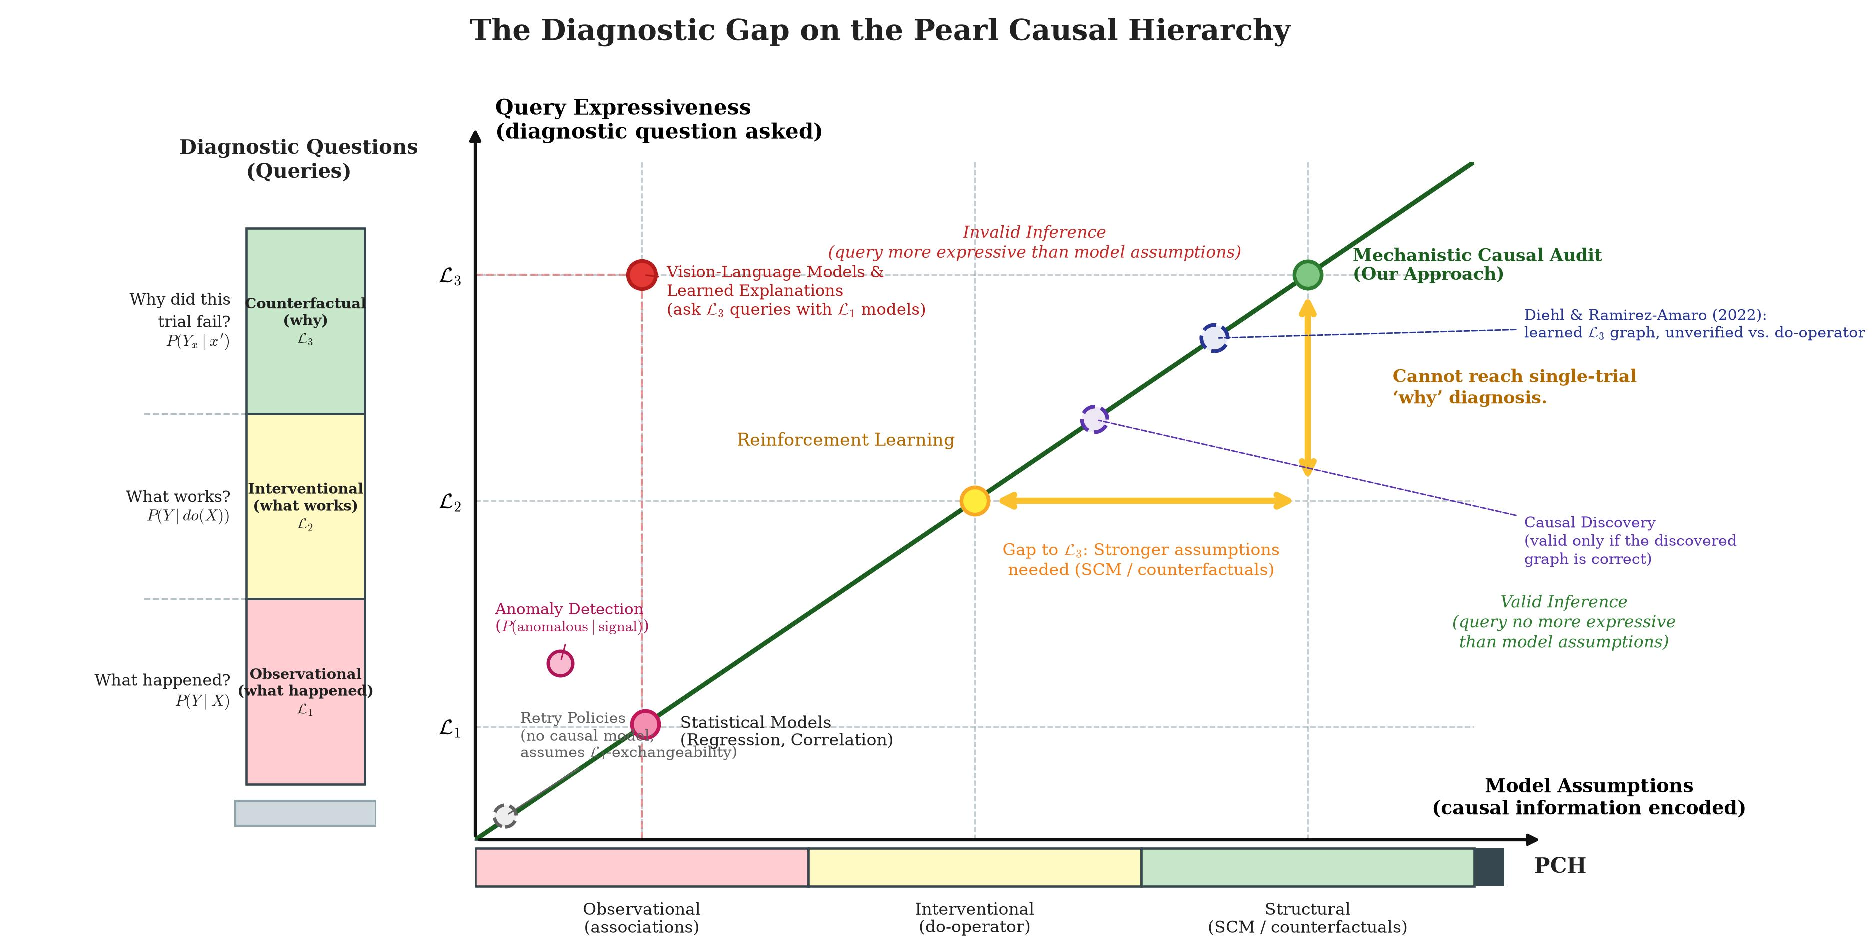
\includegraphics[width=\linewidth,trim=0 0 0 25pt,clip]{results/figures/fig_diagnostic_gap_cropped.pdf}
  \captionsetup{font=footnotesize}
  \captionof{figure}[The diagnostic gap on the Pearl Causal Hierarchy]{The diagnostic gap on the Pearl Causal Hierarchy, adapted from Yang and Bareinboim~\cite{yang2025hierarchy}. VLM explanations lie above the Cartwright line; the proposed audit matches an $\mathcal{L}_3$ query with an $\mathcal{L}_3$ model.}
  \label{fig:diagnostic_gap}
\end{minipage}
\par\medskip

Learned causal explanation methods generate post-hoc rationales for failure, but these rationales are not checked against a ground-truth counterfactual and so cannot be verified as correct.

\noindent Vision language models can describe a failed trial in natural language and propose a plausible cause, but their explanations are associative and are not tested against what would actually have happened under intervention. Chapter~\ref{ch:background} reviews these approaches in detail. What remains absent is an audit method that (a)~uses the known computational architecture of the robot to build a structural model of failure and (b)~validates that model using a principled counterfactual test to ask: \emph{if this particular structural precondition had been met, would the grasp have succeeded?} Figure~\ref{fig:diagnostic_gap} situates these approaches on the Pearl Causal Hierarchy to make the diagnostic gap geometric. In this graph, only a match between model assumptions and query expressiveness yields valid inference.

\section{The Mechanistic Causal Audit}
\label{sec:approach}

This thesis addresses the diagnostic gap by formulating grasp failure diagnosis as a mechanistic causal audit (Figure~\ref{fig:audit_engine}). Rather than attempting to statistically learn a causal graph from noisy observational data, we use the known dataflow of the robot's perception-action pipeline to pre-register a Structural Causal Model (SCM)~\cite{pearl2009causality}.

\noindent To conduct this audit, we construct a fully controlled factorial experiment in MuJoCo that implements Pearl's do-operator. This environment allows us to isolate and manipulate four exogenous environmental variables: depth noise~$\sigma_d$, point cloud retention fraction~$\rho$, camera elevation~$\phi$, and camera azimuth~$\theta$. The SCM links these controlled interventions to the binary grasp outcome~$Y$ through intermediate mechanistic variables: point cloud completeness~$C_{pc}$, grasp confidence~$q_{\text{grasp}}$, grasp pose error~$e_{\text{pose}}$ and the number of valid grasp candidates~$n_{\text{grasps}}$.

\noindent The audit is conducted entirely in simulation. The counterfactual test at the centre of this thesis rewinds a trial and re-executes it under an altered condition to obtain ground truth. No physical robot allows this, but simulation makes this possible. Therefore our conclusions describe failure mechanisms within a physically grounded simulation pipeline, but their transfer to physical hardware is not evaluated here.

\begin{figure}[t]
  \centering
  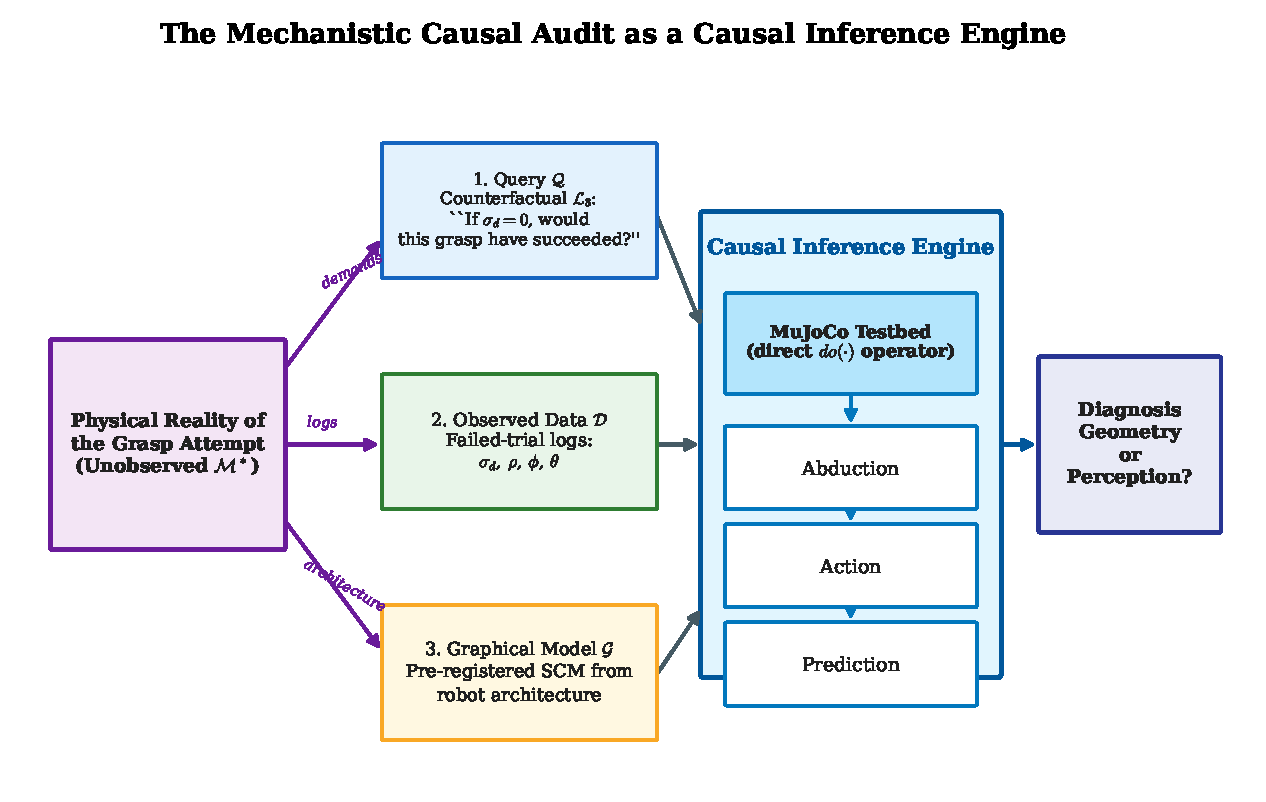
\includegraphics[width=\textwidth]{results/figures/fig_mechanistic_audit_engine.pdf}
  \caption{The Mechanistic Causal Audit framed as a causal inference engine (adapted from Yang and Bareinboim~\cite{yang2025hierarchy}). By deriving the graphical model directly from the robot's known computational architecture, the MuJoCo simulation can act as a valid inference engine, applying Pearl's three-step procedure (abduction, action, prediction) to diagnose single trial failures against ground truth.}
  \label{fig:audit_engine}
\end{figure}


\noindent To separate layers of failure, we carry out filtered and unfiltered experiments to isolate collisions and pose quality. The main factorial study executes Contact-GraspNet’s best pose and records whether that pose is already in collision - this shows how much failure is geometric vs. perceptual. We then test pose quality with a floating gripper not the full arm, so that full-arm inverse kinematics cannot confound the outcome. Without filtering, colliding poses dominate and success rate of grasps is low. We carry out a second experiment to filter collisions (a precondition that CGN's pipeline implicitly assumes) then also select a favourable viewpoint after inspecting the main grid results.

\noindent That order is itself a result of the execution stack. A first full-arm inverse-kinematics attempt reached the proposed pose and still failed to lift, for contact and gripper-geometry reasons unrelated to perception; a later logged arm pass could reach collision-filtered poses but still did not lift without listed contact compromises (Chapter~\ref{ch:method}; Appendix~\ref{app:implementation}). The floating gripper is the confirmatory validator because it isolates pose quality. Unfiltered top-1 physical execution on the full grid is the confirmatory audit of deployed pose selection (5.0\% success; 72.8\% pre-grasp collision, under the shake disturbance). Filtering is a gate intervention, not the grid on which perceptual degradations are studied: at one post-hoc clean cell it reaches 89\% under clamp-and-lift. The 5.0\% and 89\% figures are different protocol slices, not two readings of the same experiment.

Given an observed grasp failure, we apply Pearl's three-step counterfactual procedure~\cite{pearl2018book} (\emph{abduction}, \emph{action} and \emph{prediction}) to identify which modelled environmental factor most likely caused the failure. Because we fully control the exogenous variables ($\sigma_d$, $\rho$, $\phi$, $\theta$), abduction recovers only the unobserved noise terms of the intermediate structural equations. The diagnostic work is carried by the action and prediction steps, which ask what would have happened to \emph{that specific failed trial} under a different setting of one variable. This remains an $\mathcal{L}_3$ query---it conditions on the realised outcome, which a purely interventional model cannot do---and Section~\ref{sec:counterfactual_diagnosis} states this formally. And since the pipeline directly implements the do-operator, we are able to establish whether fixing the identified perceptual variable would have saved the grasp, or whether the failure was irreducibly constrained by physical geometry. The trial's random seed is recorded and held fixed on rewind, so that only the intervened-on variable changes and every other stochastic element of the pipeline replays identically. This is abduction carried out physically rather than by solving an equation---the recorded seed \emph{is} the abducted noise realisation---and it is what licenses reading the re-simulated outcome as the true counterfactual for that specific trial.


As a secondary comparison, we contrast this structured causal diagnosis against a zero-shot large language model (LLM) baseline, to illustrate what associative natural-language reasoning misses relative to a diagnosis grounded in the pipeline's known structure. The underlying model (Gemini~2.5~Flash) is VLM-capable; in this comparison, however, it receives only structured textual descriptions of each trial rather than images. The comparison is asymmetric since the SCM encodes the pipeline's architecture and the comparison measures the value of that encoding. On identical proximity-pilot failure cases, we test whether SCM-based counterfactual reasoning identifies the root cause of a grasp failure or correctly recognises that no single cause suffices more reliably than a zero-shot LLM.

\section{Aim and Objectives}
\label{sec:aims}

\paragraph{Aim.} To determine whether a pre-registered and revised mechanistic Structural Causal Model enables auditable diagnosis of robotic grasp failure, including multi-causal failures checked against simulated ground truth. The criterion against which a diagnosis is judged correct is formalised in Section~\ref{sec:single_cause_def}. As a secondary aim, we compare this structured diagnosis against a zero-shot large language model given the same observational data, to quantify what explicit structural knowledge of the pipeline contributes relative to associative natural-language reasoning. That comparison is scored on the proximity-pilot outcome; the confirmatory claims concern the physical-outcome decomposition.

\paragraph{Objectives.} To pursue this aim, we first construct a physics-grounded MuJoCo testbed capable of executing automated grasp trials under controlled perceptual degradations to establish how much failure is attributable to geometry alone, including characterising pre-grasp collision as a baseline failure mode and quantifying the effect of top-$k$ collision filtering under clean conditions. We then pre-register a Structural Causal Model whose causal graph is derived from the pipeline's known dataflow, stating in advance the conditions under which the model would be falsified. Structural equations for the intermediate mechanisms are fitted parametrically and checked against nonparametric, model-free estimates. Pearl's abduction-action-prediction procedure is applied to observed failures to identify root causes---including recognising failures that are multi-cause or irreducible---and each diagnosis is validated against simulated ground-truth counterfactuals. Finally, as a secondary comparison, the SCM's diagnoses are contrasted with those of a zero-shot LLM given identical observational data from the proximity pilot, to quantify what explicit structural knowledge contributes over associative reasoning.

\section{Contributions}
\label{sec:contributions}

The core contributions of this thesis are:

\begin{enumerate}
    \item \textbf{A Mechanistic Structural Causal Model:} An SCM for grasp failure that is derived directly from system architecture, featuring four independently intervenable variables and four measurable intermediate variables.
    \item \textbf{A Fully Controlled Factorial Testbed:} A complete simulation environment in MuJoCo~\cite{todorov2012mujoco} that directly implements Pearl's do-operator. It combines Contact-GraspNet~\cite{sundermeyer2021contact}, varied object geometries and a floating-gripper test (shake on the main grid; clamp-and-lift on the filtered clean-cell check) to eliminate confounders and isolate perceptual from geometric failures. The testbed uses a two-arm experimental design (unfiltered top-1 vs.\ filtered top-$k$), not two robot arms.
    \item \textbf{Separation of Geometry from Perception:} Geometry driven invalid poses are shown to dominate failure without collision filtering. Once these poses are gated out, the testbed achieves a high clean-condition success rate (89\%, at a favourable viewpoint selected post-hoc), confirming that it does not artificially suppress performance.
    \item \textbf{Quantification of Irreducible Multi-Causal Failures:} A counterfactual ground-truth study on the 432-trial proximity pilot (not the floating-gripper grid) shows that, within the intervention magnitudes tested, 57.2\% of failures resist single-variable attribution, concentrated at overhead viewpoints. Whether this rate is a property of the failure modes themselves or of the intervention grid is taken up in Chapter~\ref{ch:discussion}.
    \item \textbf{Counterfactual Evaluation Pipeline:} An end-to-end pipeline executes Pearl's counterfactual procedure to diagnose failures against simulated ground truth and, as a secondary contribution, compares this structured causal diagnosis against LLM-based attribution on identical proximity-pilot cases.
\end{enumerate}

\section{Structure of this Thesis}
\label{sec:organisation}

The remainder of this thesis is organised as follows.

Chapter~\ref{ch:background} reviews the theoretical background needed to motivate the audit: prior work on robotic grasp failure and approaches to failure diagnosis, Structural Causal Models and Pearl's counterfactual hierarchy, depth sensor noise and the point-cloud representation, Contact-GraspNet as the perception backbone under study, and the use of large language models in robotics.

Chapter~\ref{ch:formulation} formalises the problem. It specifies the pre-registered causal graph, the structural equations linking exogenous variables to the grasp outcome, the identifiability assumptions required for counterfactual inference, the conditions under which the SCM could be falsified, and the research hypotheses tested in later chapters.

Chapter~\ref{ch:method} describes the experimental testbed: the per-trial pipeline from camera positioning to outcome evaluation, the factorial grid over $\sigma_d$, $\rho$, $\phi$, and $\theta$, and the data-collection protocol.

Chapter~\ref{ch:diagnosis} describes the diagnostic procedure: fitting the surrogate Structural Causal Model, Pearl's abduction--action--prediction attribution, the LLM baseline comparison, and the evaluation metrics.

Chapter~\ref{ch:results} reports the confirmatory three-stage physical decomposition and the collision-filtering ceiling check. The SCM-fit, counterfactual ground-truth, and LLM numbers in that chapter are a method demonstration on the proximity pilot, including the quantification of multi-cause and irreducible failures.

Chapter~\ref{ch:discussion} interprets these results against the thesis's aim and objectives, and considers their implications and limitations.

Chapter~\ref{ch:conclusion} summarises the contributions of the thesis and outlines directions for future work.

Appendix~\ref{app:implementation} records the engineering process, including the reconstruction of the simulation environment, the iterative development of the control pipeline, and the significant bugs encountered and resolved along the way.


% ============================================================
%  CHAPTER 2: BACKGROUND AND RELATED WORK
% ============================================================
\chapter{Background and Related Work}
\label{ch:background}

This chapter reviews prior work only as far as it bears on the diagnostic gap identified in Section~\ref{sec:diagnostic_gap}: the absence of a method that both derives a structural model of failure from known architecture and checks that model's counterfactual predictions against ground truth. We first survey grasp failure and recovery (Section~\ref{sec:bg_grasp}) and the existing families of diagnosis approaches (Section~\ref{sec:bg_diagnosis}); the latter is the chapter's central argument and is organised around a single question for each family---what does it claim, what layer of the Pearl Causal Hierarchy can it answer a query at, and what can it not verify? Section~\ref{sec:bg_scm} then introduces the causal machinery the audit itself requires: Structural Causal Models, the do-operator, and Pearl's counterfactual procedure. Sections~\ref{sec:bg_depth} and~\ref{sec:bg_cgn} scope the two pipeline components under audit---the depth-noise surrogate, the point-cloud representation, and Contact-GraspNet---to exactly what the experimental design manipulates, rather than surveying sensing or grasping broadly. Section~\ref{sec:bg_llm} reviews LLMs in robotics and motivates their role here as a deliberately asymmetric baseline rather than a competing perception system.

\section{Robotic Grasp Failure and Recovery}
\label{sec:bg_grasp}

Grasp synthesis has moved from analytical methods based on force- and form-closure to data-driven models that learn proposals directly from sensor observations. Learned planners such as GraspNet-1Billion~\cite{fang2020graspnet} and Contact-GraspNet~\cite{sundermeyer2021contact} represent the current state of the art and achieve strong performance-but, as Section~\ref{sec:motivation} noted, under lab preconditions: clean sensing, a favourable viewpoint, and, as Section~\ref{sec:bg_cgn} details, a collision-filtering stage that is often left implicit. When the input point cloud is sparse, noisy, or incomplete, these models produce proposals that can be geometrically infeasible, and nothing in their design distinguishes a confidently wrong proposal from a confidently correct one.

Two mechanisms exist for handling failure once it occurs, and neither is diagnosis. Tactile feedback (e.g.\ GelSight-based systems~\cite{calandra2018more}) detects slippage \emph{during} execution, after contact is made; it cannot say why a vision-based proposal was wrong \emph{before} contact, which is where the failure modes studied in this thesis originate. Retry policies re-attempt the same or a perturbed grasp, implicitly treating failure as stochastic; if the true cause is systematic-a viewpoint that consistently fails to observe a critical surface, say-retrying reproduces the same failure at the same rate, because nothing about the violated precondition has changed. Neither mechanism asks, let alone answers, \emph{which} precondition of success was violated. Failures stay undecomposed.

A related line of work seeks to raise success rates by adapting perception during execution, rather than attributing failure after the fact. Active perception methods such as ActiveVLA~\cite{liu2026activevla} adapt viewpoint and resolution to improve success; this thesis instead treats viewpoint (and other perceptual degradations) as intervenable causes and asks whether failures can be diagnosed via a mechanistic SCM. The two questions are complementary: ActiveVLA asks how to look better so that a policy succeeds; this thesis asks, given that a grasp already failed under a fixed viewpoint and sensing regime, which controlled factor was responsible.

\section{Approaches to Grasp Failure Diagnosis}
\label{sec:bg_diagnosis}

Section~\ref{sec:diagnostic_gap} listed six families of response to grasp failure, each addressing part of the problem while stopping short of a full structural account. This section expands that list one family at a time, applying the same three questions to each: what does the method claim, what layer of the Pearl Causal Hierarchy (Figure~\ref{fig:diagnostic_gap}) can it answer a query at, and what can it not verify?

\textbf{Retry strategies.} Claim: repeating a grasp under fresh stochastic variation~\cite{hsiao2010contact} will eventually succeed if the original failure was due to chance. PCH layer: none, strictly---retry is not a model of the failure at all, only repeated sampling, and it implicitly assumes $\mathcal{L}_1$-exchangeability of outcomes across attempts. Cannot verify: whether the failure was in fact stochastic or systematic in the first place, which is exactly the discrimination this thesis needs to make and that retry assumes away.

\textbf{Anomaly detection.} Claim: a trial's force/torque or tactile signature is unusual relative to a learned reference distribution~\cite{park2018multimodal}. PCH layer: $\mathcal{L}_1$---it computes an associational judgement, $P(\text{anomalous} \mid \text{signal})$. Cannot verify: which upstream variable produced the anomaly, or what would have happened had that variable taken a different value; detecting that something is wrong is not the same as attributing why.

\textbf{Reinforcement learning.} Claim: a policy trained on past failures~\cite{levine2018learning, kalashnikov2018scalable} reduces their future frequency. PCH layer: $\mathcal{L}_2$ at best---the policy's weights implicitly encode something like $P(Y \mid \doop(\text{action}))$, aggregated across training experience. Cannot verify: any explicit, human-checkable account of why one specific trial failed; the ``explanation'' is distributed across millions of parameters, and there is no single-trial counterfactual query that can be put to it.

\textbf{Causal discovery.} Claim: a causal graph can be recovered from purely observational trial data by testing conditional independencies. PCH layer: in principle $\mathcal{L}_2$--$\mathcal{L}_3$, \emph{if} the discovered graph happens to be correct. Cannot verify: the correctness of the discovered graph itself, which depends on independence-test power, sample size, and the absence of unmeasured confounding---conditions robotics trial data rarely satisfy, and that need not be satisfied here at all, because the pipeline's dataflow (camera $\to$ point cloud $\to$ CGN $\to$ kinematics) is already known by construction. Statistically re-discovering an architecture that is already certain discards information rather than substituting for its absence.

\textbf{Causal robot-failure explanation.} This is the closest prior work to the present thesis in query type, so the contrast is worth stating precisely rather than in general terms. Diehl and Ramirez-Amaro~\cite{diehl2022whydidifail} learn a causal Bayesian network from simulation data and generate contrastive explanations by searching for the nearest counterfactual state that would have succeeded---a genuinely $\mathcal{L}_3$-style query, sharing this thesis's goal of structural causal explanation. Three differences separate the two approaches. First, their graph is \emph{learned} by structure search, ours is \emph{pre-registered} from the pipeline's known computational architecture (Section~\ref{sec:approach}), so ours carries none of the discovery risk raised in the previous paragraph. Second, their target is a manipulation \emph{policy} on tasks such as block-stacking, evaluated on task-level success, whereas ours audits a fixed, pre-trained perception-to-planning \emph{pipeline}, evaluated on the validity of a single upstream grasp proposal. Third, their counterfactual is produced by a contrastive nearest-state search over the learned model itself, ours by Pearl's explicit abduction--action--prediction procedure (Section~\ref{sec:counterfactual_diagnosis}), checked against re-simulated ground truth obtained by actually rewinding the trial via the do-operator, rather than against the model's own self-consistency. What their setting cannot verify, and ours can: that the nearest contrastive state found by the search is also the \emph{true} counterfactual, since there is no simulated do-operator ground truth available to check it against. CausalWorld~\cite{ahmed2021causalworld} similarly exposes intervenable causal variables in a manipulation simulator and could in principle supply such ground truth, but is built for transfer learning and policy generalisation; it answers ``how do these variables affect training performance'' rather than ``which variable caused this specific trial's failure.''

\textbf{Vision-language models.} Claim: an LLM or VLM prompted with a description of a failure proposes a plausible cause in natural language~\cite{ahn2022saycan, driess2023palm}. PCH layer: $\mathcal{L}_1$ only---the model was trained on associations between descriptions and outcomes, and its explanation is a language-model completion conditioned on text, not a computation over a structural model. Cannot verify: the causal correctness of its own explanation; by construction, an $\mathcal{L}_1$ model cannot answer an $\mathcal{L}_3$ query no matter how fluent it sounds (Cartwright's ``no causes in, no causes out''~\cite{cartwright1989}; Figure~\ref{fig:diagnostic_gap}). Section~\ref{sec:bg_llm} reviews the broader use of LLMs in robotics and motivates their specific role here as a baseline that makes this asymmetry visible, not as a competing perception system.

Across all six families, the same two ingredients are missing together, and no method reviewed above supplies both: (a)~a structural model derived from the pipeline's own known architecture, rather than discovered from data or foregone entirely, and (b)~validation of that model's counterfactual predictions against ground truth obtained by actually rewinding and re-executing the trial, rather than against the model's own predictions. Figure~\ref{fig:diagnostic_gap} places these six families on the Pearl Causal Hierarchy; the point the reviewed literature does not reach is the one this thesis occupies. Supplying (a) and (b) together is the task of the remainder of this chapter and of Chapter~\ref{ch:formulation}.

\section{Structural Causal Models and Counterfactuals}
\label{sec:bg_scm}

Section~\ref{sec:bg_diagnosis} argued that no reviewed method combines a pre-registered structural model with counterfactual validation against ground truth. This section introduces the formal apparatus needed to build and validate one: the SCM formalism, the do-operator, the Pearl Causal Hierarchy, and Pearl's three-step counterfactual procedure.

Structural Causal Models, developed by Pearl~\cite{pearl2009causality}, provide a rigorous mathematical foundation for reasoning about cause and effect. The causal structure is represented as a \emph{directed acyclic graph} (DAG), where each node corresponds to a variable and each directed edge $V_i \to V_j$ indicates that $V_i$ is a direct cause of $V_j$ in the model. An SCM assigns a structural equation to each node, formalising the mechanism by which a variable is produced from its graph-theoretic parents.

\begin{definition}[Structural Causal Model]
A Structural Causal Model is a triple $\SCM = (\mathbf{U}, \mathbf{V}, \mathbf{F})$ where:
\begin{itemize}
  \item $\mathbf{U}$ is a set of \emph{exogenous} (background) variables whose values are determined by factors outside the model.
  \item $\mathbf{V} = \{V_1, V_2, \ldots, V_n\}$ is a set of \emph{endogenous} variables whose values are determined by the structural equations.
  \item $\mathbf{F} = \{f_1, f_2, \ldots, f_n\}$ is a set of \emph{structural equations}, where each $f_i$ expresses $V_i$ as a function of its parent variables (a subset of $\mathbf{V} \cup \mathbf{U}$): $V_i = f_i(\text{pa}(V_i), U_i)$.
\end{itemize}
\end{definition}

\paragraph{The do-operator and interventional reasoning.}
Causal effects are formalised via the \emph{do-operator}: the expression $\doop(X = x)$ denotes an intervention that sets variable $X$ to value $x$ by removing all incoming edges to $X$ in the causal graph and fixing its value, regardless of what its structural equation would normally produce~\cite{pearl2009causality}. The distinction between the do-operator and ordinary conditioning is fundamental. The conditional probability $P(Y \mid X = x)$ reflects both causal and non-causal (e.g., confounded) associations between $X$ and $Y$. The interventional distribution $P(Y \mid \doop(X = x))$ reflects only the causal effect of $X$ on $Y$, because the intervention removes the influence of confounders that act through $X$'s parents.

\paragraph{The Pearl Causal Hierarchy.}
These three modes of reasoning---observational, interventional, and counterfactual---correspond to the three layers of the \emph{Pearl Causal Hierarchy} (PCH)~\cite{pearl2009causality}: $\mathcal{L}_1$ (seeing: $P(Y \mid X)$), $\mathcal{L}_2$ (doing: $P(Y \mid \doop(X))$), and $\mathcal{L}_3$ (imagining: $P(Y_x \mid x')$). Yang and Bareinboim~\cite{yang2025hierarchy} formalise this hierarchy through a corresponding sequence of graphical model classes---Bayesian Networks, Causal Bayesian Networks, and Counterfactual Bayesian Networks---and prove that each level encodes strictly stronger constraints than those below, with a commensurate reduction in empirical falsifiability. This thesis operates at $\mathcal{L}_3$: the counterfactual queries in Chapter~\ref{ch:formulation} ask what \emph{would} have happened to a specific observed trial under a hypothetical change to conditions, which requires the full expressive power of the SCM. Every family reviewed in Section~\ref{sec:bg_diagnosis} either lacked the structural assumptions to license an $\mathcal{L}_3$ query (retry, anomaly detection, RL, VLMs) or lacked a pre-registered, architecture-derived graph even where it reached $\mathcal{L}_3$ in principle (causal discovery, learned causal explanation); this is precisely why $\mathcal{L}_3$ diagnosis needs structural assumptions stated in advance, not inferred from the same data the diagnosis is meant to explain.

\paragraph{Pre-registered versus discovered graphs.} Section~\ref{sec:bg_diagnosis} distinguished two ways a graph can be obtained: discovered from data---by statistical causal discovery, or by structure search as in Diehl and Ramirez-Amaro~\cite{diehl2022whydidifail}---or pre-registered from known architecture. This thesis takes the second path throughout: Chapter~\ref{ch:formulation} states the graph of Figure~\ref{fig:causal_dag} before any diagnostic use is made of it, and Section~\ref{sec:falsification} reports the pre-specified tests that could have, and in two instances did, contradict it. Pre-registration does not make the graph immune from being wrong; it makes being wrong a testable event rather than an unfalsifiable modelling choice.

\paragraph{Parametric versus non-parametric SCMs, and what this thesis commits to.} Vonk et al.~\cite{vonk2023disentangling} distinguish SCMs specified \emph{non-parametrically}, where each $f_i$ is left as an arbitrary function and only qualitative properties (e.g.\ monotonicity) are assumed, from SCMs specified \emph{parametrically}, where a functional form is fixed in advance. Non-parametric specification is preferable when feasible, because it avoids functional-form misspecification, but arbitrary functions cannot be estimated from finitely many trials without additional structure. This thesis separates two decisions that are often bundled together. The \emph{graph} $\mathcal{G}$---which variables are causes of which---is pre-registered from the pipeline's known computational architecture, as just discussed; it is not discovered, and it is not left unspecified. The \emph{mechanisms} $f_i$ (Section~\ref{sec:structural_equations}) are fitted \emph{parametrically}, as linear-in-parameters regressions with a logistic link for the binary outcome. This parametric commitment on the mechanisms is deliberate, not a default, and its cost is stated explicitly in Section~\ref{sec:structural_equations}: any true non-linearity not captured by the chosen basis functions will surface as model misspecification rather than as noise. To keep this parametric surrogate honest rather than assumed, every structural equation's linear-in-parameters prediction is checked against a \emph{nonparametric}, model-free estimate---stratified means and Wilson-score proportions computed directly on the factorial grid, with no line fitted to them (Section~\ref{sec:falsification})---and any divergence between the two is reported as a located failure of the surrogate rather than smoothed into the residual. The graph, in short, is the pre-registered, falsifiable object that this thesis's diagnostic claims rest on; the mechanisms are a scoped parametric surrogate for that graph's edges, whose fidelity is checked non-parametrically rather than assumed. Two consequences follow. First, the count variable $n_{\text{grasps}}$ has a point mass at zero---Contact-GraspNet returns no candidate at all on $141/432$ trials, concentrated at severe noise---which a linear-Gaussian equation cannot represent: ``CGN found nothing to grasp'' and ``CGN found a corrupted pose'' are mechanistically distinct events with plausibly different causes, and this thesis models the count as a two-part hurdle (Section~\ref{sec:structural_equations}). Second, wherever a specific functional form was found to overreach---most notably the $q_{\text{grasp}} \to e_{\text{pose}}$ term, which Section~\ref{sec:causal_graph} shows is not a mediation edge---the term is removed rather than kept and explained away. Full nonparametric checks are reported in \texttt{results/scm\_nonparametric\_report.md}.

\subsection{Pearl's Three-Step Counterfactual Procedure}

Counterfactual reasoning extends interventional reasoning by asking questions about specific individuals or events: \emph{given what actually happened, what would have happened if conditions had been different?} Pearl's three-step procedure~\cite{pearl2018book} formalises this:

\begin{enumerate}
  \item \textbf{Abduction.} Given the observed evidence $\mathbf{e}$ (the values of all measured variables in the actual world), infer the values of the exogenous noise terms $\mathbf{U}$ that are consistent with $\mathbf{e}$. In a deterministic SCM, this amounts to solving the structural equations for the noise terms:
  \begin{equation}
    U_i = V_i^{\text{obs}} - f_i(\text{pa}(V_i)^{\text{obs}}).
    \label{eq:abduction}
  \end{equation}
  This step ``personalises'' the model to the specific observed instance.

  \item \textbf{Action.} Apply the hypothetical intervention $\doop(X = x')$ to the model by replacing the structural equation for $X$ with the constant assignment $X = x'$.

  \item \textbf{Prediction.} Propagate the modified structural equations forward, using the abducted noise terms from Step~1, to compute the counterfactual outcome $Y_{X=x'}$.
\end{enumerate}

The counterfactual outcome $Y_{X=x'}$ is the value that $Y$ \emph{would have taken} in the specific observed instance if $X$ had been set to $x'$ instead of its actual value, with all other exogenous factors held at their abducted values. This is a statement about a specific individual event, not a population-level statistic. It is this apparatus-a graph fixed in advance, and mechanisms whose functional form is stated and checked rather than left to be inferred from the same outcome data the diagnosis is meant to explain-that makes single-trial counterfactual diagnosis possible, and that Chapter~\ref{ch:formulation} instantiates for this pipeline.

\section{Depth Sensing and Point Clouds}
\label{sec:bg_depth}

A depth buffer is a two-dimensional array in which each element stores the perpendicular distance, in metres, from the camera's focal point to the nearest surface visible at that pixel. Real depth sensors exhibit stochastic axial noise whose magnitude grows with distance and angle of incidence: Khoshelham and Elberink~\cite{khoshelham2011accuracy} report standard deviations of approximately 1--2\,mm at 1\,m rising to roughly 40\,mm at 5\,m for a structured-light sensor, and Nguyen et al.~\cite{nguyen2012modeling} show that the accompanying lateral component is typically larger still. A physically faithful model of this kind is not what the experimental design in Chapter~\ref{ch:formulation} needs. The additive Gaussian model $d_{\text{noisy}} = d_{\text{true}} + \mathcal{N}(0, \sigma_d^2)$ is adopted here as the standard first-order surrogate used in depth-simulation pipelines, for one specific reason: it exposes a single, continuously variable, independently intervenable parameter $\sigma_d$ that can be set to a chosen value on every trial, which a physically complete sensor model-with its coupled distance-, angle-, and material-dependent terms-would not.

This is a deliberate scoping decision, not an oversight, and its causal role in this pipeline is fixed empirically rather than assumed. Section~\ref{sec:falsification} shows that $\sigma_d$ has no measurable effect on point cloud completeness $C_{pc}$, because $C_{pc}$ is computed from the segmentation buffer before noise is injected, but has direct effects on grasp confidence $q_{\text{grasp}}$, candidate count $n_{\text{grasps}}$, and pose error $e_{\text{pose}}$: noise acts on what Contact-GraspNet does with the points it receives, not on how many points it receives. What this scoping does not give: any claim about a specific real depth camera's behaviour, or about the non-Gaussian effects (specular dropout, edge bias) that a full sensor model would include. $\sigma_d$ is a controllable surrogate for the intervention this thesis actually runs, not a sensor model in its own right.

A \emph{point cloud} is the geometric object obtained by back-projecting a depth buffer through the pinhole camera model, and it is the primary input to Contact-GraspNet. It is this object whose quality the four causal variables $(\sigma_d,\, \rho,\, \phi,\, \theta)$ degrade.

\begin{definition}[Point Cloud]
\label{def:pointcloud}
A point cloud $\mathcal{P}$ is a finite, unordered set of vectors in
three-dimensional Euclidean space:
\begin{equation}
  \mathcal{P} = \bigl\{\, \mathbf{p}_i \in \mathbb{R}^3 \;\big|\; i = 1, \ldots, N \,\bigr\},
  \label{eq:pointcloud_def}
\end{equation}
where each element $\mathbf{p}_i = (X_i,\, Y_i,\, Z_i)^\top$ encodes the
three-dimensional Cartesian coordinates of a single surface sample, and $N$ is
the total number of samples.
\end{definition}

Several properties of this definition deserve emphasis.  First, the point cloud
has no inherent topological structure: there are no edges, faces, or connectivity
relations between the points.  Each point is an independent geometric measurement.
Second, the set is unordered: permuting the indices $i$ yields the same point cloud.
This distinguishes a point cloud from an image, where pixel $(u,v)$ has a fixed
neighbourhood.  Third, the point cloud is \emph{partial}: it contains only those
surface locations that are visible from the camera's viewpoint and within the
sensor's measurement range.  Points on occluded or distant surfaces are absent.

This last property is not a deficiency but a physically accurate representation
of what a depth sensor observes from a single viewpoint.  Real-world depth sensors
such as the Intel RealSense D400 series and the Microsoft Kinect produce exactly
this structure: a set of metric surface samples from the sensor's perspective.
The point cloud formalises this. A retained fraction $\rho$ of these points is written $\mathcal{P}_\rho$; the sampling rule is specified in Chapter~\ref{ch:method}.

Grasp poses predicted from a point cloud are typically expressed in the OpenCV camera convention ($+Z$ forward, $+Y$ down); MuJoCo's cameras follow OpenGL ($+Z$ backward, $+Y$ up). Conversion between the two is an implementation detail of Chapter~\ref{ch:method}.

\section{Contact-GraspNet}
\label{sec:bg_cgn}

Contact-GraspNet (CGN)~\cite{sundermeyer2021contact} is a neural network for 6-DoF grasp generation from point-cloud observations: given a partial point cloud $\mathcal{P}$, it outputs a set of grasp proposals, each a $4\times4$ pose together with a scalar confidence, by predicting per-point contact probability rather than regressing poses from global point cloud features. Its architecture processes each point $\mathbf{p}_i$ through a PointNet++-style encoder~\cite{qi2017pointnetpp} that aggregates local geometric features by grouping neighbouring points in 3D space. For each point, the network then predicts whether it is a valid contact point for a parallel-jaw gripper and, if so, what the associated grasp pose should be. This contact-centric formulation is architecturally anchored to the point cloud: the network's prediction heads are defined \emph{per point in $\mathcal{P}$}, not per image pixel or per voxel. Providing the raw depth image or a mesh instead would require a fundamentally different model. Using the point cloud is therefore not a design choice made in this thesis but a prerequisite of using CGN.

CGN was trained on partial point clouds generated from single-viewpoint depth renders of ShapeNet objects~\cite{sundermeyer2021contact}---precisely the same modality as the perception pipeline in this thesis---under clean sensing conditions (no depth noise, no extreme viewpoint). A full mesh or a CAD model of the target object would be \emph{out of distribution} for CGN: the network has never been trained to process complete, noise-free geometric representations. Using the partial, viewpoint-dependent point cloud produced by back-projection faithfully reproduces the input distribution on which CGN was trained, which is essential for the validity of any degradation study. A degradation that pushes the input away from the training distribution for a reason unrelated to the variable under study would confound the causal analysis. CGN's headline accuracy-over 90\% on unseen objects in structured clutter-is reported downstream of a collision-aware selection stage that filters candidate grasps before execution.

That filtering stage is frequently left implicit in how such numbers are quoted, yet it is itself a precondition of success rather than a detail: without it, poses that are in collision with the object or support surface are counted alongside geometrically valid ones, and success rates collapse for reasons that have nothing to do with perception. This observation motivates the two-arm experimental design of Chapter~\ref{ch:method} (Section~\ref{sec:approach}), which separates an unfiltered arm (raw geometric validity under top-1 execution; this is the confirmatory grid, on which perceptual degradations are studied) from a filtered arm (top-$k$ collision rejection as a gate intervention) precisely so that this often-implicit precondition is measured rather than assumed away.

For this thesis, CGN is treated strictly as a fixed black-box backbone: its architecture is not modified or retrained, and the object of study is how its outputs-confidence $q_{\text{grasp}}$, candidate count $n_{\text{grasps}}$, and pose error $e_{\text{pose}}$-respond to controlled perturbation of its inputs, namely point cloud completeness $C_{pc}$ (via viewpoint) and depth noise $\sigma_d$ (via the surrogate of Section~\ref{sec:bg_depth}). Framed this way, CGN's opacity as a deep network is not the diagnostic problem this thesis solves: the SCM does not need to open CGN up, only to model its input-output behaviour as a mechanism with measurable intermediate variables, which is the surrogate-model move formalised in Section~\ref{sec:scm_fitting}. What CGN's opacity does foreclose is any diagnosis that depends on inspecting its internals directly-attention maps or learned features offered as an explanation-and that route is deliberately not taken here.

\section{Large Language Models in Robotics}
\label{sec:bg_llm}

SayCan~\cite{ahn2022saycan}, Code as Policies~\cite{liang2023code}, and VoxPoser~\cite{huang2023voxposer} show that LLMs can plan, generate control code, and compose 3D value maps for manipulation, and PaLM-E~\cite{driess2023palm} extends this to a jointly trained vision-language model. Common to all four is that they operate at the task-planning level and take correct upstream perception as given; none has a mechanism to diagnose \emph{why} perception itself failed once it has. That is a different question from the one this thesis asks, and evaluating an LLM as a diagnostic system, rather than as a planner, requires a different protocol from the one these systems were built for.

Used as a diagnostic baseline (Section~\ref{sec:llm_baseline}), an LLM's explanation is an $\mathcal{L}_1$ completion conditioned on a textual description of the trial: fluent, but not the output of a structural computation, and not checked against any counterfactual by construction (Section~\ref{sec:bg_diagnosis}). The comparison in this thesis is deliberately asymmetric rather than a fair fight between equally-equipped systems: the LLM used (Gemini~2.5~Flash) is VLM-capable, but is given only structured text, not images, so that the comparison isolates the value of \emph{structural knowledge of the pipeline} rather than the value of extra perceptual input or raw model capability. The LLM is given the same observational facts the SCM has access to (Tiers T1--T3, Section~\ref{sec:llm_baseline}) and is asked to do, associatively, what the SCM does structurally; any gap between the two is then attributable to the structural model, not to a difference in what each system was shown. Asymmetry here is intentional: the point of the comparison is not to find out which system is more capable in general, but what explicit structural knowledge of the pipeline is worth, holding the available information fixed.

% ============================================================
%  CHAPTER 3: PROBLEM FORMULATION
% ============================================================
\chapter{Problem Formulation}
\label{ch:formulation}

This chapter formalises grasp failure diagnosis as a causal inference problem. We define the variables, specify the causal graph, state the structural equations, state the conditions under which the model would be falsified then finally state the research hypotheses.

\section{Variables}
\label{sec:variables}

Four \emph{exogenous} variables <$\sigma_d$, $\rho$, $\phi$, $\theta$> are set by the experimenter in each trial.  <$\sigma_d$, $\rho$> describe the quality of the depth measurement: $\sigma_d$ is the per-pixel standard deviation (metres) of Gaussian noise applied to the rendered depth image after clipping negative values to zero while $\rho$ is the fraction of 3D points retained after that noisy depth is back projected to a point cloud. <$\phi$, $\theta$> describe where the observation is made from, where $\phi$ is the camera elevation above the horizontal and $\theta$ its azimuth, both on a fixed radius sphere centred on the object. Together these exogenous variables quantify sensor degradation and partial observability. A trial with large $\sigma_d$ and small $\rho$ gives CGN a corrupted and sparse point cloud, whereas one at steep $\phi$ presents a clean cloud that conceals the object's vertical surfaces. The four variables are mutually independent by construction and graphically <$\sigma_d,\rho,\phi,\theta$> have no parents in the DAG (hence the name exogenous) \\

\noindent Five \emph{endogenous} variables <$C_{pc}$, $n_{\text{grasps}}$, $q_{\text{grasp}}$, $e_{\text{pose}}$, $\text{has\_grasps}$> are measured within each trial. Segmentation fraction $C_{pc}$ is the fraction of image pixels belonging to the target object, computed from the simulator's segmentation buffer - a low $C_{pc}$ means the object is poorly resolved. The name is a slight misnomer worth flagging once: $C_{pc}$ is a 2-D segmentation-mask pixel fraction computed \emph{before} the 3-D point cloud is formed, which is precisely why depth noise and downsampling---both point-cloud-stage manipulations---turn out to have no causal effect on it (Section~\ref{sec:falsification}). The name is retained for continuity with the codebase and prior sections of this thesis rather than introduced fresh here. The remaining variables characterise CGN's output. The gate $\text{has\_grasps} \in \{0,1\}$ records whether CGN returns any candidate grasp at all; $n_{\text{grasps}}$ is the number of grasps returned; $q_{\text{grasp}}$ is the confidence score assigned to the top-ranked candidate grasps; and $e_{\text{pose}}$ is the Euclidean distance in the horizontal plane between that candidate's gripper $(x,y)$ and the true object centroid, so a large $e_{\text{pose}}$ means a grasp was proposed far from the object it should hold.~The outcome $Y \in \{0,1\}$ is binary grasp success or failure.~The gate is treated separately because when $\text{has\_grasps}=0$ there is no pose to execute and $n_{\text{grasps}}$, $q_{\text{grasp}}$, $e_{\text{pose}}$ are undefined for that trial. \\

\noindent Each structural equation carries its own exogenous \emph{noise term} $U_i$ ($U_C, U_q, U_n, U_e$) representing unmodelled factors internal to that mechanism such as segmentation noise, CGN's internal stochasticity or pose regression error. The independence of these noise terms determines whether the model is Markovian in the sense required by Section~\ref{sec:counterfactual_diagnosis}. This thesis uses ``exogenous'' in two related but distinct senses. In the graphical sense, $\sigma_d$, $\rho$, $\phi$, $\theta$ are exogenous because they have no parents in the DAG. Separately, each structural equation carries its own exogenous noise term $U_i$. It is the independence properties of these noise terms, not of the four controlled variables, that determine whether the model is Markovian in the sense required by the counterfactual identification argument of Section~\ref{sec:counterfactual_diagnosis}.

\section{Causal Graph}
\label{sec:causal_graph}

The causal relationships are encoded in the DAG of Figure~\ref{fig:causal_dag}. The graph was derived by reading the execution order of our experimental pipeline, not from inspecting \texttt{experiment\_results.csv}. Each edge justified as ``the code that computes $Y$ reads the value of $X$'', following Section~\ref{sec:bg_scm} - and only afterwards checked interventionally against the data (Section~\ref{sec:falsification}). Four assumptions define it.

\begin{enumerate}
  \item $\sigma_d$ and $\rho$ are \emph{not} parents of $C_{pc}$, so $C_{pc}$ is affected by viewpoint ($\phi,\theta$) only. This is because $C_{pc}$ is computed from the segmentation buffer and is rendered before noise injection and downsampling, therefore neither variables can affect it. Both edges were pre-registered and have since been falsified (Section~\ref{sec:falsification}).

  \item The gate $\text{has\_grasps}$ is caused directly by all four exogenous variables and is \emph{not} mediated through $C_{pc}$. This is the primary causal claim of the SCM. CGN's forward pass reads the full 3-D point cloud, which carries $\sigma_d$ and $\rho$ as well as viewpoint, whereas $C_{pc}$ is only a 2-D mask fraction; $\phi,\theta$ therefore have two separate downstream paths rather than one routed through the other.

  \item $n_{\text{grasps}}$ is caused by all four exogenous variables; $q_{\text{grasp}}$ by all four plus $n_{\text{grasps}}$, where for the latter the reported score is the maximum over a pool of size $n_{\text{grasps}}$, so a larger pool mechanically raises the expected maximum. $e_{\text{pose}}$ is affected by all four variables directly, through the camera-to-world transform that determines which surfaces are visible and where the proposed pose lands.

  \item There is \emph{no} $q_{\text{grasp}} \to e_{\text{pose}}$ edge, despite the two covarying. Both are read from the same $\arg\max$ index of the same set of scored candidates; the code that computes the pose never reads the score. They are siblings under a common unobserved parent correlated through a shared selection index. An earlier draft treated $q_{\text{grasp}}$ as a mediator of $e_{\text{pose}}$, but that framing is retracted (Section~\ref{sec:falsification}). This is a dataflow provable instance of the independent errors (NPSEM-ie) assumption failing for one specific pair, which Section~\ref{sec:counterfactual_diagnosis} returns to.
\end{enumerate}

\noindent Finally, $\text{has\_grasps}=0$ forces $Y=0$ directly. Conditional on $\text{has\_grasps}=1$, the confirmatory $Y$ is a physical hold/lift of the object (Section~\ref{sec:success_criterion_detail}), not a proximity threshold on $e_{\text{pose}}$. The confirmatory estimand is unfiltered top-1 execution: the highest-scoring pose is placed with the hand open, and a pre-grasp collision is recorded rather than skipped. Top-$k$ collision filtering is a separate intervention on that gate, not the default of the factorial grid. The pre-registered graph in Figure~\ref{fig:causal_dag} does not include this collision gate as a node; that omission is discussed in Chapter~\ref{ch:discussion}.

\begin{figure}[t]
  \centering
  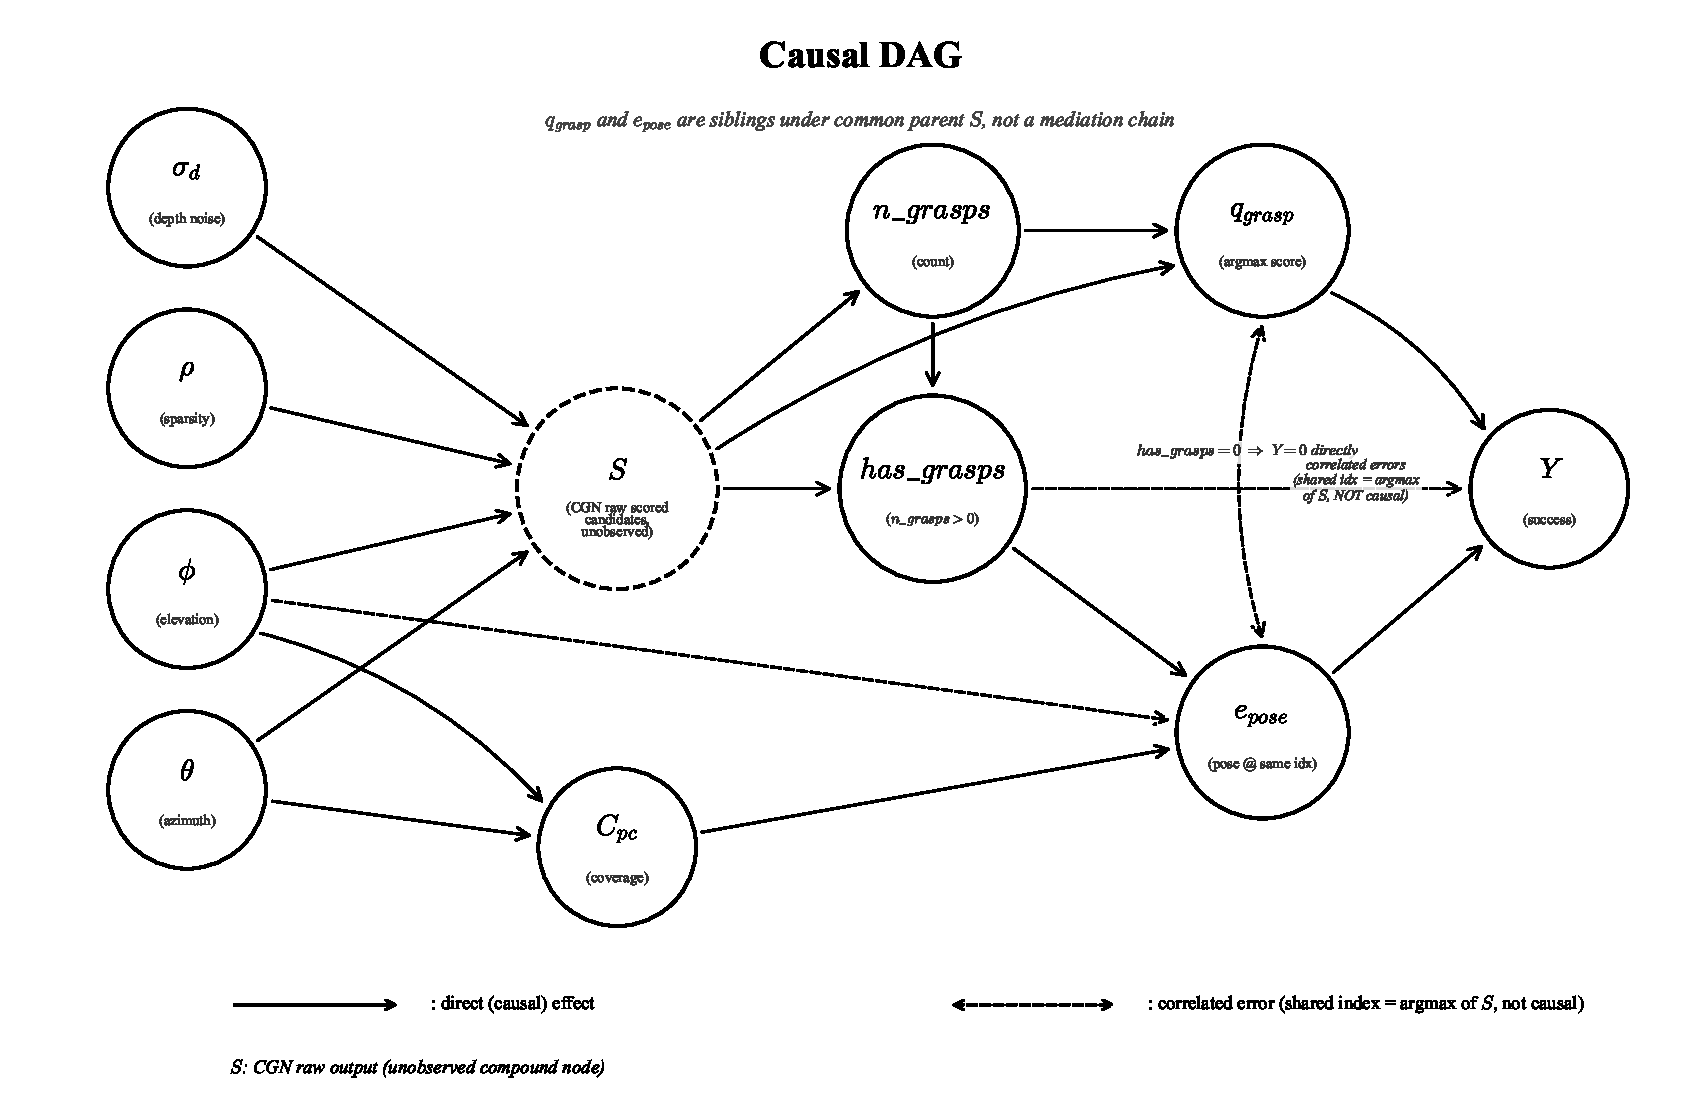
\includegraphics[width=\textwidth]{results/figures/causal_dag.pdf}
  \caption{Causal DAG, pre-registered (\texttt{CAUSAL\_DAG\_PREREGISTRATION.md}) and corrected after the falsification tests of Section~\ref{sec:falsification}. $\sigma_d,\rho$ have no direct edge into $C_{pc}$; $\text{has\_grasps}$ is the primary causal node and is not mediated through $C_{pc}$; $q_{\text{grasp}}$ and $e_{\text{pose}}$ are siblings with correlated errors (dashed, non-causal); $\text{has\_grasps}=0$ forces $Y=0$.}
  \label{fig:causal_dag}
\end{figure}

\section{Structural Equations}
\label{sec:structural_equations}

The mechanisms presented below are parametrised as a small set of regression models chosen for interpretability, not to represent the true mechanism exactly (they are not claims about the true functional form). Only the graph of Section~\ref{sec:causal_graph} carries the falsifiable commitment that this report's diagnostic claims depend on (Section~\ref{sec:bg_scm}). . Two specification choices follow from the graph. First, $n_{\text{grasps}}$ has a point mass at zero---CGN returns no candidate at all on 141 of 432 trials---so it is modelled as a two-part hurdle-a gate, and a count conditional on the gate---rather than one continuous equation that would blur the distinction of Assumption 2. Second, $q_{\text{grasp}}$ and $e_{\text{pose}}$ are specified as siblings, so neither equation contains the other as a regressor.

\begin{align}
  C_{pc} &= \beta_0 + \beta_1\phi + \beta_2\theta + U_C \label{eq:cpc}\\[2pt]
  P(\text{has\_grasps}=1) &= \sigma\!\left(\eta_0 + \eta_1\sigma_d + \eta_2\rho + \eta_3\phi + \eta_4\theta\right) \label{eq:hg}\\[2pt]
  n_{\text{grasps}} \mid \text{has\_grasps}{=}1 &\sim \text{NegBin}\!\left(\exp(\zeta_0 + \zeta_1\sigma_d + \zeta_2\rho + \zeta_3\phi + \zeta_4\theta),\, \kappa\right) \label{eq:ng}\\[2pt]
  q_{\text{grasp}} &= \gamma_0 + \gamma_1\sigma_d + \gamma_2\rho + \gamma_3\phi + \gamma_4\theta + \gamma_5\log n_{\text{grasps}} + U_q \label{eq:qg}\\[2pt]
  e_{\text{pose}} &= \delta_0 + \delta_1\sigma_d + \delta_2\rho + \delta_3\phi + \delta_4\theta + U_e \label{eq:ep}
\end{align}

Equations~\eqref{eq:ng}--\eqref{eq:ep} are fitted only on trials clearing the gate. $n_{\text{grasps}}$ is modelled as an overdispersed count because raw candidate counts are non-negative and right-skewed. The $\log n_{\text{grasps}}$ term in~\eqref{eq:qg} is the order-statistic correction of Assumption 3; omitting it would let the exogenous coefficients absorb a pool-size effect unrelated to grasp quality. Functional forms are kept plain, and each equation's prediction is checked against a model-free estimate computed directly on the factorial grid (\texttt{results/scm\_nonparametric\_report.md}); divergences are reported as located failures of the surrogate rather than absorbed into higher-order terms added after the fact. Flexible parameterisations are identified as future work in Chapter~\ref{ch:discussion}.

$Y$ is not fitted as its own regression. $Y=0$ whenever $\text{has\_grasps}=0$; conditional on the gate, $Y$ is determined by the success criterion of Section~\ref{sec:success_criterion_detail}. Under the historical proximity criterion used to fit the equations above, this reduces to a near-deterministic threshold on $e_{\text{pose}}$ (97.9\% agreement with the logged post-execution outcome, Section~\ref{sec:scm_fit}), meaning $Y$ and $e_{\text{pose}}$ are two measurements of nearly the same quantity rather than an independent cause-effect pair. This is a measurement limitation and is why the redesigned floating-gripper outcome (Section~\ref{sec:approach}) is used for the primary results of Chapter~\ref{ch:results}. An earlier draft specified $Y$ as a logistic function of $q_{\text{grasp}}$, $n_{\text{grasps}}$ and $e_{\text{pose}}$ jointly; that equation is retracted for the same reason.

The dataset comprises 432 trials in total; six (1.4\%) terminated with a file-locking race condition in the logging layer and have no recorded outcome (Section~\ref{sec:limitations}), leaving 426 with a usable outcome for every equation fitted above. The plain linear term in Equation~\eqref{eq:cpc} accounts for 89.3\% of the variance in $C_{pc}$ over $\phi \in [30°, 60°]$ (Section~\ref{sec:scm_fit}); a trigonometric transform of $\phi$ (e.g.\ $\sin\phi$) was considered and is not used. At $\phi = 30°$, CGN consistently proposes positions approximately 6\,cm from the true centroid, even with clean inputs; intervening on $\phi$ changes $e_{\text{pose}}$, so this is a causal effect of viewpoint on pose error. Fitting $e_{\text{pose}}$ on a log scale was considered as a robustness check and did not change the sign or ranking of any coefficient, so the untransformed scale is retained for direct interpretability in metres. Downstream of the gate, success itself is decomposed as $P(Y{=}1) = P(\text{has\_grasps}{=}1) \times P(Y{=}1 \mid \text{has\_grasps}{=}1)$, so that ``no proposal was found'' and ``a proposal was found but executed poorly'' are scored as two distinct causal pathways. \label{sec:eq_gate}

\section{Falsification Conditions}
\label{sec:falsification}

A model that could not in principle be contradicted by data is not a model of the pipeline but a restatement of the researcher's assumptions. We therefore state in advance what would count as evidence against the graph. Two objects must be kept distinct: the MuJoCo\,+\,CGN simulator is treated as ground truth throughout; the SCM is a model \emph{of} that simulator, and it is the SCM that is on trial.

Each non-edge in Figure~\ref{fig:causal_dag} is a testable conditional-independence claim. The absence of $\sigma_d \to C_{pc}$, for example, implies $\sigma_d$ carries no additional explanatory power for $C_{pc}$ once $\phi,\theta$ are controlled. Because the four exogenous variables are assigned by design rather than sampled, each such test is interventional ($\mathcal{L}_2$), not merely observational. Table~\ref{tab:falsification} reports the pre-specified tests, run against the 426-trial analysis sample (full detail in \texttt{results/dag\_edge\_falsification\_report.md}).

\begin{table}[t]
  \caption{Pre-specified falsification tests of the causal graph.}
  \label{tab:falsification}
  \centering
  \small
  \begin{tabular}{p{5.3cm}p{4.7cm}l}
    \toprule
    \textbf{Claim tested} & \textbf{Test} & \textbf{Verdict} \\
    \midrule
    $\sigma_d \to C_{pc}$ & Partial coefficient, controlling $\rho,\phi,\theta$ & \textbf{Falsified} ($p=0.938$); edge removed \\
    $\rho \to C_{pc}$ & Partial coefficient, controlling $\sigma_d,\phi,\theta$ & \textbf{Falsified} ($p=0.986$); edge removed \\
    $\phi \to C_{pc}$, $\theta \to C_{pc}$ & Partial coefficients & Confirmed ($p<0.001$) \\
    Mutual independence of $\sigma_d,\rho,\phi,\theta$ & Pairwise correlation across grid & Confirmed (max $|r| < 10^{-4}$) \\
    $\sigma_d,\rho,\phi,\theta \to \text{has\_grasps}$ & Coefficient significance in Eq.~\eqref{eq:hg} & Confirmed for $\sigma_d,\phi,\theta$ ($p<0.001$); \textbf{not detected} for $\rho$ ($p=0.144$) at $n=426$ \\
    $q_{\text{grasp}} \to e_{\text{pose}}$ & Dataflow reading of \texttt{best\_grasp\_cam} & \textbf{Falsified}; siblings, not mediation; edge removed \\
    \bottomrule
  \end{tabular}
\end{table}

Three of the seven pre-specified tests came back against the pre-registered graph. Two concern $C_{pc}$: the original specification asserted all four exogenous variables affect the target object's segmentation fraction, but this is wrong for this pipeline, because the segmentation buffer is rendered before noise injection and downsampling. The graph and Equation~\eqref{eq:cpc} were revised to remove both edges rather than retaining them and letting the discrepancy vanish into $U_C$. The $\rho \to \text{has\_grasps}$ edge is retained despite a non-significant coefficient at $n=426$, because it is implied directly by dataflow (fewer points can only reduce the chance of identifying a graspable region); the null is flagged as limited statistical power, not confirmation of no effect.

The third, the $q_{\text{grasp}} \to e_{\text{pose}}$ edge, cannot be settled statistically. Conditioning on $\{\sigma_d,\rho,\phi,\theta,\log n_{\text{grasps}}\}$ still leaves a significant residual coefficient ($n=285$; coefficient $-0.184$, $p=0.015$), which is what a confounded sibling pair would both produce, since a chain and a fork with a shared parent are indistinguishable from conditioning alone. What settles the direction is the code: the function returning the pose never reads the score, and both are read from the same $\arg\max$ index. The residual correlation is confirmed, but as evidence \emph{for} the sibling reading. Separately, the fitted equations' predictions of $P(Y \mid \doop(v))$ are checked against stratified, model-free estimates computed with no line fitted to them; the divergence at $\phi=30°$, where CGN exhibits a systematic pose bias that a single global slope cannot represent, is reported directly rather than smoothed over. Together these conditions fix in advance what would count against the model, and record that some of it did, so the SCM's later agreement with ground truth (Chapter~\ref{ch:results}) is not circular.

\paragraph{(b) Held-out interventional predictions.} Beyond conditional-independence tests on the graph's structure, the fitted structural equations make quantitative predictions about $P(Y \mid \doop(v))$ that can be checked against a statistic computed independently of the OLS/logistic fit itself: the stratified, model-free total-effect and path-decomposition estimates reported in \texttt{results/scm\_nonparametric\_report.md} (means and Wilson-score proportions computed directly from the factorial grid, with no line fitted to them). Where a structural equation's linear-in-parameters prediction diverges from this model-free estimate---as it does for the CGN pose bias at $\phi=30°$ discussed in Section~\ref{sec:structural_equations}---this divergence is reported as a specific, located failure of the parametric surrogate rather than smoothed over.

\section{Single-Cause, Multi-Cause, and Irreducible Failure}
\label{sec:single_cause_def}

Hypothesis~\ref{hyp:accuracy} and Contribution 4 both depend on a precise definition of ``single cause'', so we fix it here. For an observed failure with conditions $\mathbf{x}^* = (\sigma_d^*,\rho^*,\phi^*,\theta^*)$ and $Y^*=0$, let $Y(v \!\to\! v_{\text{nom}})$ denote the outcome obtained by resetting exogenous variable $v$ alone to its nominal clean-baseline value ($\sigma_d = 0$, $\rho = 1.0$, $\phi = 45°$, $\theta = 0°$) while holding the other three at their observed values. The failure is \textbf{single-cause} with respect to $v$ if $Y(v \!\to\! v_{\text{nom}})=1$ for exactly one $v$; \textbf{multi-cause} if for more than one; and \textbf{irreducible} (reported as \texttt{none}) if for none.

Three properties of this definition matter for interpreting the results. It is anchored to a specific intervention \emph{magnitude} - a full reset to baseline, not a graded correction - so the reported irreducibility rate describes failures resisting this class of intervention, not irreducibility in any magnitude-independent sense. It is also anchored to a specific choice of $\phi_{\text{nom}}$ ($45°$, rather than the other two sampled elevations), and a failure attributed to $\phi$ under one baseline elevation could be classified differently under another (e.g.\ $\phi_{\text{nom}} = 30°$). Chapter~\ref{ch:discussion} returns to both sensitivities. Finally, $Y(v \!\to\! v_{\text{nom}})$ is obtained from simulated ground truth, by re-simulation with the trial's seed held fixed where available---physical abduction, Section~\ref{sec:approach}---and only otherwise from the fitted surrogate - which additionally requires a rank-preservation assumption on the abducted noise term (Section~\ref{sec:counterfactual_diagnosis}): that the trial's position in the noise distribution, once solved for under the observed condition, is preserved under the intervened-on condition. It is never read off the SCM's own prediction of itself, which is what keeps the classification from being tautological. Where re-simulated ground truth is available it is used in preference to the surrogate for exactly this reason.

This yields the correctness criterion referenced in the aim (Section~\ref{sec:aims}): a diagnosis is correct if it attributes a single-cause failure to the right variable, and recognises a multi-cause or irreducible failure as such rather than asserting a culprit the counterfactual evidence does not support.

\section{Research Hypotheses}
\label{sec:hypotheses}

\begin{hypothesis}
  Counterfactual diagnosis over the fitted SCM will attribute single-cause failures to the correct root variable in more than 50\% of test cases - a bar chosen because chance attribution among four candidates is approximately 25\%.
  \label{hyp:accuracy}
\end{hypothesis}

\begin{hypothesis}
  Causal counterfactual diagnosis will achieve higher attribution accuracy than zero-shot LLM diagnosis on the same failure cases.
  \label{hyp:comparison}
\end{hypothesis}

\begin{hypothesis}
  LLM-based attribution will be less consistent across repeated queries than the deterministic SCM-based attribution.
  \label{hyp:consistency}
\end{hypothesis}

These three hypotheses concern the diagnostic procedure of Chapter~\ref{ch:diagnosis}, which was developed on the 432-trial proximity pilot. Hypotheses~\ref{hyp:accuracy} and~\ref{hyp:comparison} are not evaluated on the confirmatory floating-gripper outcome; Hypothesis~\ref{hyp:consistency} is discussed only as a structural contrast. The confirmatory claims of this thesis are the physical-outcome decomposition, not a scored SCM-versus-LLM bake-off.

% ============================================================
%  CHAPTER 4: EXPERIMENTAL TESTBED
% ============================================================
\chapter{Experimental Testbed}
\label{ch:method}
\label{ch:testbed}

This chapter describes the experimental testbed. Perception---camera placement, depth rendering, noise injection, and Contact-GraspNet---is shared across all runs. Execution was redesigned in a strictly sequential chain, documented in Appendix~\ref{app:implementation}: a first full-arm inverse-kinematics stack failed to lift; a proximity threshold on $e_{\text{pose}}$ was used only as a 432-trial pilot; the confirmatory bed is a floating-gripper physical hold/lift test on a 7{,}560-trial factorial grid. A later full-arm due-diligence pass (Section~\ref{sec:ik_controller}) showed that reach can be solved and that a lift exists only under listed contact compromises; it was not adopted as the confirmatory outcome. No two execution protocols were run as a designed comparison; each was rejected, or scoped as due diligence, only after a located failure mode.

\section{Pipeline Overview}
\label{sec:pipeline_overview}

Each confirmatory trial follows Algorithm~\ref{alg:pipeline}. Perception is shared with the 432-trial pilot; execution uses the floating-gripper protocol of Section~\ref{sec:grasp_execution}. The two early exits implement the $\text{has\_grasps}$ gate of Section~\ref{sec:causal_graph}: an empty segmentation or a zero candidate count sets $Y=0$ without execution. The remainder of this chapter expands the camera, depth, point-cloud, transform, and execution steps in the same order.

\begin{algorithm}[hbt!]
\caption{Confirmatory Trial Simulation Pipeline}
\label{alg:pipeline}
\begin{algorithmic}[1]
\Require Object scene $S$, exogenous settings $(\sigma_d, \rho, \phi, \theta)$, seed
\Ensure Binary outcome $Y$; mediators $(C_{pc}, q_{\text{grasp}}, n_{\text{grasps}}, e_{\text{pose}})$; collision flag
\State Load $S$; reset to the home configuration; park the arm; settle the object; \texttt{mj\_forward}
\State Place camera at $(\phi, \theta)$ on the $0.8$\,m sphere about the settled centroid
\State $D \gets \mathrm{RenderDepth}(480 \times 640)$; \quad $M \gets \mathrm{RenderSegmentation}()$
\State $C_{pc} \gets |\{p : M_p = \mathrm{target}\}|/(480 \times 640)$ \Comment{from $M$, before noise}
\If{$C_{pc} = 0$}
    \State $Y \gets 0$; log row; \textbf{return} \Comment{no visible object}
\EndIf
\State $D_{\mathrm{noisy}} \gets \max(0,\, D + \mathcal{N}(0,\sigma_d^2))$ \Comment{i.i.d.\ per pixel; identity if $\sigma_d=0$}
\State $\mathcal{P} \gets \mathrm{BackProject}(D_{\mathrm{noisy}}, K)$ \Comment{camera frame}
\State $\mathcal{P}_{\rho} \gets \mathrm{StridedDownsample}(\mathcal{P}, \rho)$
\State $\{P_i, s_i\}_{i=1}^{n_{\text{grasps}}} \gets \mathrm{ContactGraspNet}(\mathcal{P}_{\rho})$
\If{$n_{\text{grasps}} = 0$}
    \State $Y \gets 0$; log row; \textbf{return} \Comment{$\mathrm{has\_grasps}=0$}
\EndIf
\State $i^* \gets \arg\max_i s_i$; \quad $q_{\text{grasp}} \gets s_{i^*}$; \quad $P_{\mathrm{cam}} \gets P_{i^*}$
\State $P_{\mathrm{world}} \gets T_{\mathrm{cam}}^{\mathrm{world}}\, F\, P_{\mathrm{cam}}$ \Comment{Section~\ref{sec:frame_transform}}
\State $e_{\text{pose}} \gets \bigl\lVert \mathrm{pos}_{xy}(P_{\mathrm{world}}) - \mathrm{centroid}_{xy} \bigr\rVert_2$ \Comment{logged mediator}
\State Load floating-gripper scene; copy the settled object pose
\If{open-hand pose collides}
    \State $Y \gets 0$ \Comment{pre-grasp gate}
\Else
    \State Close fingers; apply lift/shake (Section~\ref{sec:grasp_execution})
    \State $Y \gets \mathbf{1}\{\text{held in footprint and lift threshold met throughout disturbance}\}$
\EndIf
\State Log exogenous settings, mediators, collision flag, and $Y$ to CSV
\end{algorithmic}
\end{algorithm}

\section{Camera Positioning and Virtual Viewpoint}
\label{sec:camera_positioning}

The perception camera is mounted on a body (\texttt{perception\_camera\_body}) defined in the MuJoCo scene XML. This body has no mass and does not participate in contact dynamics. At each trial, the body's position and orientation are set programmatically to place the camera at the desired viewpoint on the viewing sphere.

The camera position is computed from the spherical coordinates $(\phi, \theta, r)$ as:
\begin{align}
  x_{\text{cam}} &= x_{\text{obj}} + r \cos\phi \cos\theta, \nonumber \\
  y_{\text{cam}} &= y_{\text{obj}} + r \cos\phi \sin\theta, \label{eq:cam_pos} \\
  z_{\text{cam}} &= z_{\text{obj}} + r \sin\phi, \nonumber
\end{align}
where $(x_{\text{obj}}, y_{\text{obj}}, z_{\text{obj}}) = (0.5, 0, 0.455)$\,m is the target object centroid and $r = 0.8$\,m is the sphere radius.

The camera orientation is computed using a look-at construction. The forward direction is the unit vector from the camera position to the target:
\begin{equation}
  \hat{\mathbf{f}} = \frac{\mathbf{p}_{\text{obj}} - \mathbf{p}_{\text{cam}}}
                         {\|\mathbf{p}_{\text{obj}} - \mathbf{p}_{\text{cam}}\|}.
  \label{eq:forward}
\end{equation}
The right direction is computed as the cross product with the world up vector:
\begin{equation}
  \hat{\mathbf{r}} = \frac{\hat{\mathbf{f}} \times \hat{\mathbf{z}}_{\text{world}}}
                         {\|\hat{\mathbf{f}} \times \hat{\mathbf{z}}_{\text{world}}\|},
  \label{eq:right}
\end{equation}
and the up direction completes the orthonormal frame:
\begin{equation}
  \hat{\mathbf{u}} = \hat{\mathbf{r}} \times \hat{\mathbf{f}}.
  \label{eq:up}
\end{equation}

In MuJoCo, the camera looks along the local $-Z$ axis, with $+X$ pointing right and $+Y$ pointing up. Therefore, the rotation matrix from camera frame to world frame has columns $(\hat{\mathbf{r}}, \hat{\mathbf{u}}, -\hat{\mathbf{f}})$:
\begin{equation}
  \mathbf{R} = \begin{bmatrix} \hat{\mathbf{r}} & \hat{\mathbf{u}} & -\hat{\mathbf{f}} \end{bmatrix}.
  \label{eq:cam_rot}
\end{equation}
This rotation matrix is then converted to a unit quaternion and written to \texttt{model.body\_quat}. The virtual camera sets $\phi$ and $\theta$ exactly and independently of $\sigma_d$ and $\rho$, which is what the factorial design requires (Sections~\ref{sec:approach} and~\ref{sec:causal_graph}).

\section{Depth Rendering and Noise Injection}
\label{sec:depth_rendering}

The depth buffer is rendered using MuJoCo's built-in renderer at $480 \times 640$ pixel resolution. Noise injection is implemented as a simple additive operation:
\begin{equation}
  d_{\text{noisy}}(u, v) = \max\!\left(0,\; d_{\text{raw}}(u, v) + \epsilon(u, v)\right),
  \qquad \epsilon(u, v) \sim \mathcal{N}(0, \sigma_d^2),
  \label{eq:noise_injection}
\end{equation}
where the $\max$ operation ensures that depth values remain non-negative. The noise is drawn independently for each pixel and each trial, using a seeded random number generator (\texttt{numpy.random.default\_rng}) to ensure reproducibility.

\section{Point Cloud Generation}
\label{sec:pointcloud_definition}

The point cloud $\mathcal{P}$ of Definition~\ref{def:pointcloud} is generated by back-projecting the noisy depth image, then retaining a fraction $\rho$ of its points. The remainder of this section records those two operations and why they are cleanly separable on $\mathcal{P}$.

\subsection{Generation via Pinhole Back-Projection}
\label{sec:backprojection}

The noisy depth image is back-projected through the pinhole camera model.
Only pixels with valid depth ($0 < d(u,v) < d_{\max}$, where $d_{\max}$ is the scene far-clip distance) are used; background pixels are excluded. For a pixel at position $(u, v)$ with depth value $d = d_{\text{noisy}}(u, v)$ (after noise injection, per Equation~\eqref{eq:noise_injection}), the 3D coordinates in the camera frame are:
\begin{equation}
  X^{(\text{cam})} = \frac{(u - c_x)\, d}{f_x}, \qquad
  Y^{(\text{cam})} = \frac{(v - c_y)\, d}{f_y}, \qquad
  Z^{(\text{cam})} = d,
  \label{eq:backproject}
\end{equation}
where $(f_x, f_y)$ are the focal lengths in pixels and $(c_x, c_y)$ is the
principal point (image centre).  The focal lengths are computed analytically from
the MuJoCo vertical field-of-view $\alpha$ and image height $H$:
\begin{equation}
  f_y = \frac{H/2}{\tan(\alpha/2)}, \qquad f_x = f_y
  \label{eq:focal_from_fov}
\end{equation}
(square pixels are assumed, as MuJoCo renders with equal horizontal and vertical
angular resolution).  For the 60° vertical FOV and $H = 480$ pixels used in
this project, $f_y \approx 415.7$\,px.

The set of all such back-projected vectors, collected over valid pixels, constitutes
the camera-frame point cloud $\mathcal{P} = \{\mathbf{p}_1^{(\mathrm{cam})}, \ldots, \mathbf{p}_N^{(\mathrm{cam})}\}$
that is passed to Contact-GraspNet. Grasp poses are produced in that same camera frame
and only afterwards transformed to the MuJoCo world frame (Section~\ref{sec:frame_transform}).

\subsection{Causal Separability on the Point Cloud}
\label{sec:pointcloud_justification}

The four causal variables in this study act on the point cloud through distinct
and non-interacting mechanisms, which is the condition required for causal
identifiability~\cite{pearl2009causality}:
\begin{itemize}
  \item Depth noise $\sigma_d$ perturbs the $Z_i$ coordinate (and propagates
        proportionally to $X_i$ and $Y_i$ through the back-projection
        equations~\eqref{eq:backproject}), independently across points and trials.
  \item Sparsity $\rho$ retains a fraction $\rho$ of points from
        $\mathcal{P}$ by evenly-strided selection
        (Section~\ref{sec:pointcloud_downsampling}), reducing $N$ without
        affecting the coordinates of retained points.
  \item Camera elevation $\phi$ and azimuth $\theta$ determine which surface regions
        are visible from the viewpoint, controlling which surface locations can
        appear in $\mathcal{P}$ at all, prior to any noise or downsampling.
\end{itemize}
These operations cannot be cleanly separated on a depth image (which is a
structured 2D grid with implicit coordinate geometry), a voxel grid (where
sparsity would mean empty cells rather than missing surface samples), or a mesh
(where connectivity would be disrupted by point removal).  On the point cloud,
each operation is a well-defined algebraic transformation on $\mathcal{P}$.

\subsection{Downsampling}
\label{sec:pointcloud_downsampling}

Sparsity is operationalised as evenly-strided, order-preserving subsampling of
the back-projected cloud, not as a second random draw. Let $\mathcal{P}$ denote
the full camera-frame cloud with $N$ points, and let
$n_{\text{keep}} = \max\!\bigl(1,\, \operatorname{round}(\rho N)\bigr)$.
For $\rho < 1$ the retained index set is
\begin{equation}
  \mathcal{I}_\rho
  = \Biggl\{\,
      \operatorname{round}\!\Biggl(\frac{k\,(N-1)}{n_{\text{keep}}-1}\Biggr)
      \;\Big|\;
      k = 0, \ldots, n_{\text{keep}}-1
    \Biggr\},
  \qquad
  \mathcal{P}_\rho
  = \bigl\{\, \mathbf{p}_i \;\big|\; i \in \mathcal{I}_\rho \,\bigr\},
  \label{eq:downsampled_cloud}
\end{equation}
with duplicate indices dropped; $\rho = 1$ retains $\mathcal{P}$ unchanged.
This is implemented by \texttt{sim\_common.deterministic\_downsample\_idx} and
applied independently to the full cloud and to each object segment. Given
$(N,\rho)$ the result is seed-independent, so $\rho$ is not a second stochastic
process layered on $\sigma_d$. The 432-trial pilot instead used uniform random
subsampling without replacement (\texttt{numpy.random.Generator.choice}).

The point cloud $\mathcal{P}_\rho$ is the final output of the perception stage and
the direct input to Contact-GraspNet.  Its cardinality is
$|\mathcal{P}_\rho| \approx \rho N$, ranging from the full cloud
($\rho = 1.0$) to 25\% of the original points ($\rho = 0.25$), with
$\rho \in \{1.0, 0.75, 0.50, 0.25\}$ across the experimental grid.

\section{Contact-GraspNet Proposal Visualisation}
\label{sec:cgn_visualisation}

The downsampled and noisy point cloud is passed to Contact-GraspNet (CGN), which operates on the visible surface geometry. For a rotationally symmetric object like a cylinder, CGN proposes a dense distribution of grasp candidates covering the observed surface. 

Figure~\ref{fig:cgn_distribution} illustrates the result of this perception process under baseline clean conditions ($\sigma_d=0, \rho=1.0$). The proposed grasps form a distinct crescent or "croissant" shape when viewed from above (Figure~\ref{fig:cgn_distribution}, left). This shape is an expected and geometrically correct consequence of the camera's fixed viewpoint ($\phi=45^\circ$): the camera only observes approximately 180 degrees of the cylinder's circumference. CGN proposes valid contact points across this entire visible arc, radiating outward with approach directions orthogonal to the cylinder surface. 

\begin{figure}[htbp]
    \centering
    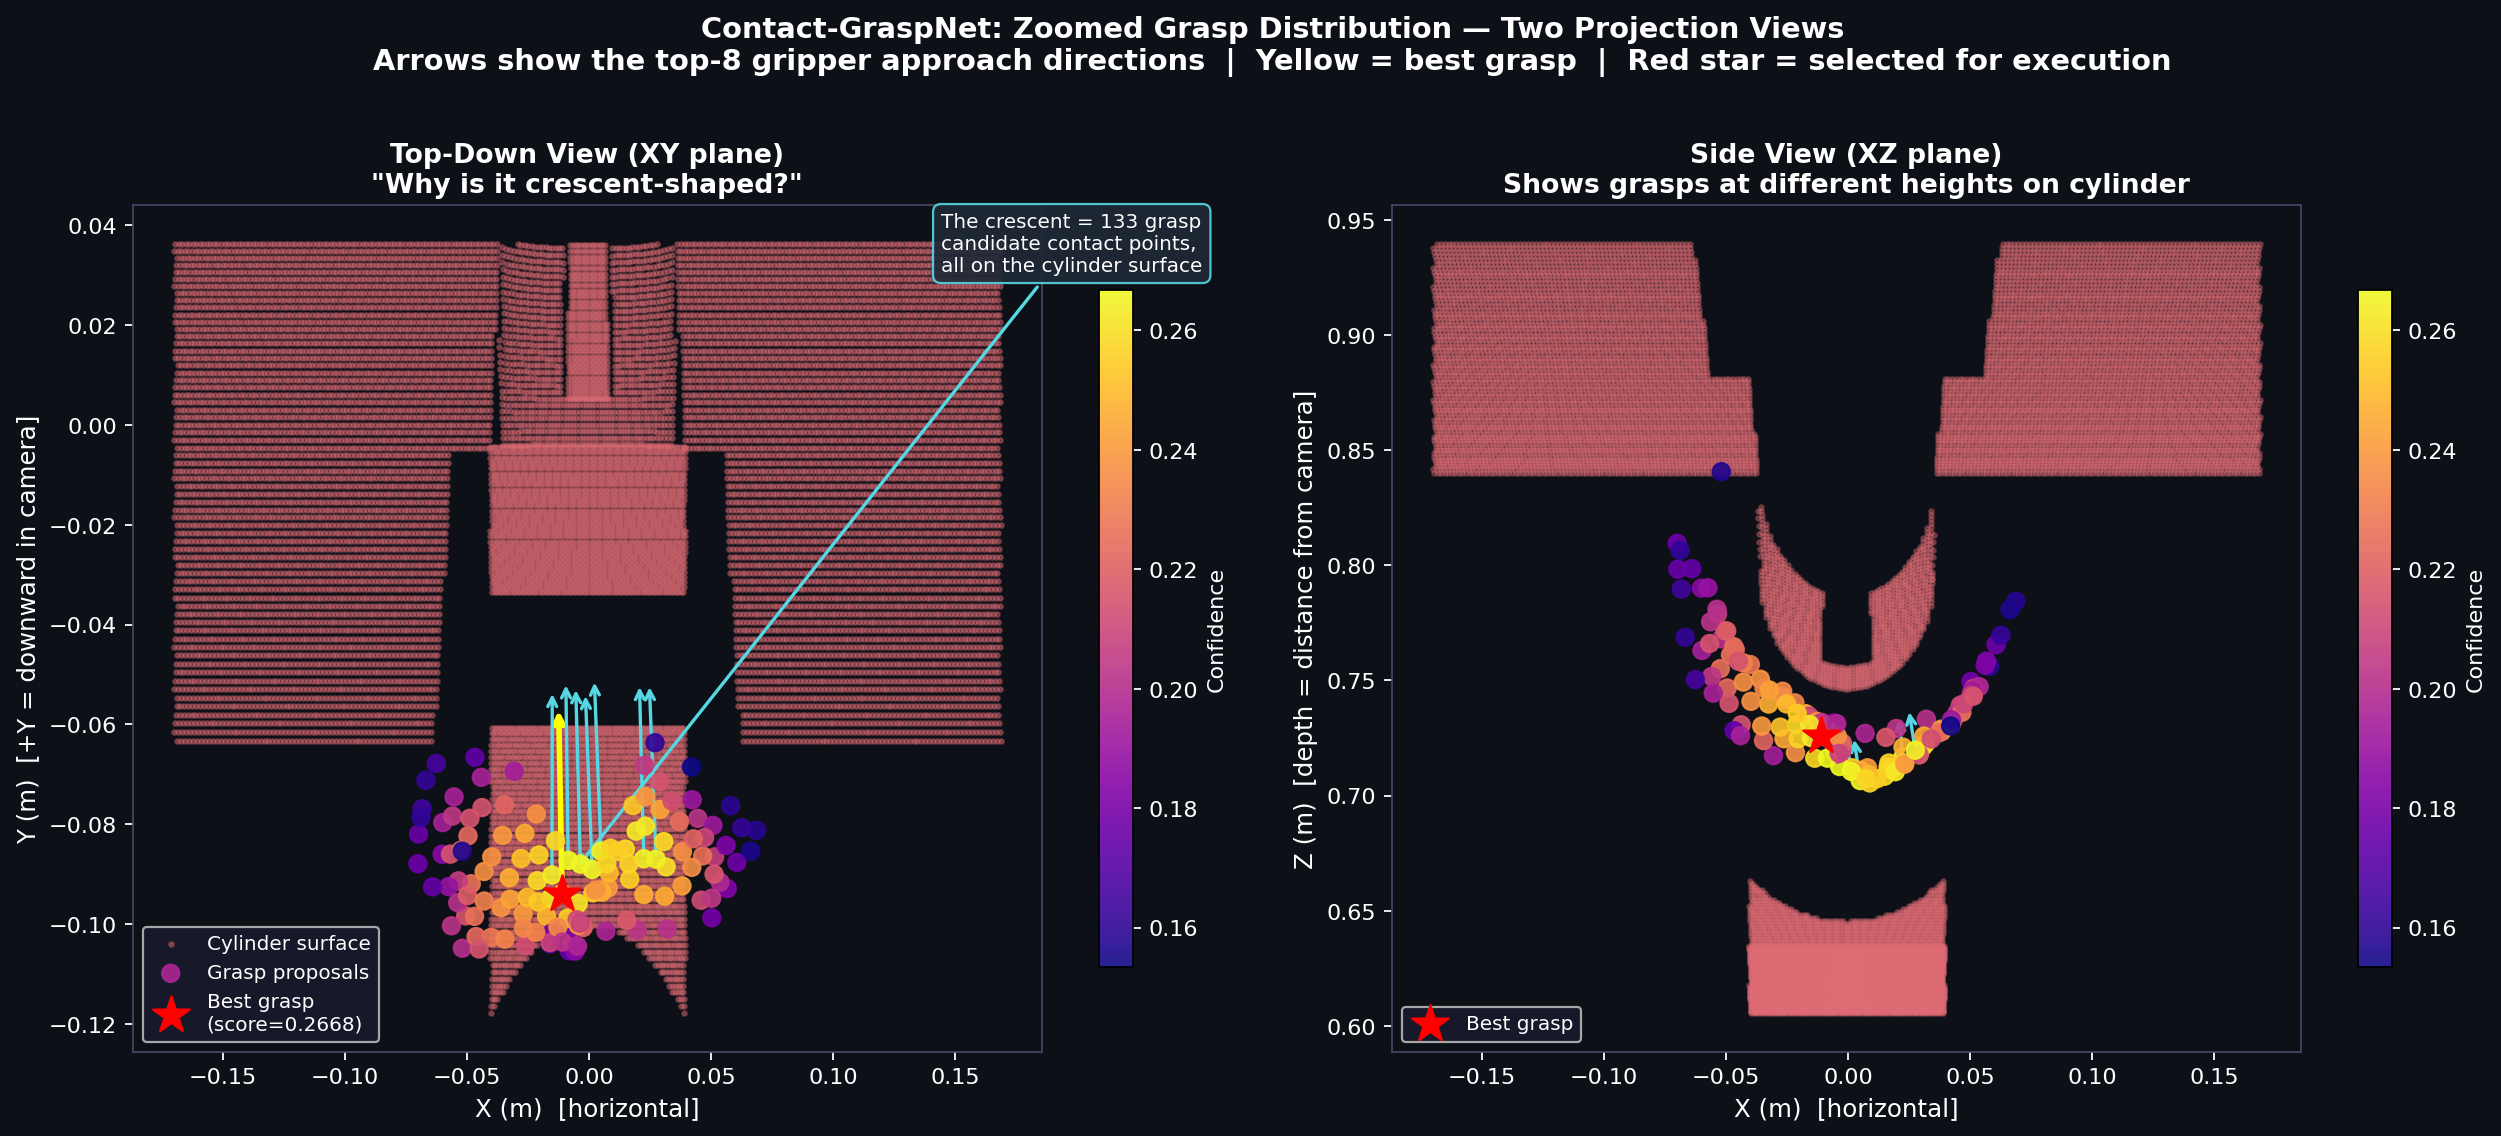
\includegraphics[width=\textwidth]{results/figures/cgn_zoomed_2d_projections.png}
    \caption{Contact-GraspNet grasp proposal distribution for the target cylinder. \textbf{Left:} Top-down (XY) projection showing the crescent of candidates on the visible surface arc. \textbf{Right:} Side (XZ) projection showing height variation. Arrows indicate the top-scoring gripper approach directions. The red star marks the single highest-confidence grasp selected for execution.}
    \label{fig:cgn_distribution}
\end{figure}

The confidence scores associated with each proposal (encoded by colour) indicate CGN's internal certainty of grasp success. The top-scoring candidate (red star) is extracted and selected for execution. As perceptual degradation variables ($\sigma_d, \rho$) are increased, this distribution becomes sparser and less confident, simulating the causal effect of poor perception on grasp synthesis.

\section{Coordinate Frame Transformation}
\label{sec:frame_transform}

The camera intrinsics used in the back-projection (Equation~\eqref{eq:backproject}) are
derived analytically from MuJoCo's vertical field-of-view parameter, as given in
Equation~\eqref{eq:focal_from_fov}.  The downsampled point cloud $\mathcal{P}_\rho$
(Equation~\eqref{eq:downsampled_cloud}) is then passed to Contact-GraspNet, which
outputs grasp poses in the camera frame.

As noted in Section~\ref{sec:bg_depth}, Contact-GraspNet follows the OpenCV camera convention and MuJoCo follows OpenGL. Conversion requires negating the $Y$ and $Z$ axes:
\begin{equation}
  \mathbf{F} = \operatorname{diag}(1,\, -1,\, -1).
  \label{eq:flip}
\end{equation}

Let $\mathbf{T} \in \mathbb{R}^{4 \times 4}$ be the homogeneous camera-to-world transform obtained from MuJoCo's \texttt{data.cam\_xmat} (the $3 \times 3$ rotation matrix stored column-major in a flat array of length 9) and \texttt{data.cam\_xpos} (the $3 \times 1$ position vector). A grasp pose $\mathbf{P}_{\text{cam}}$ in the OpenCV camera frame is transformed to the world frame as:
\begin{equation}
  \mathbf{P}_{\text{world}} = \mathbf{T} \, \mathbf{F} \, \mathbf{P}_{\text{cam}}.
  \label{eq:transform}
\end{equation}
The translation component $\mathbf{P}_{\text{world}}[:3, 3]$ gives the proposed gripper position in world coordinates, from which $e_{\text{pose}}$ is computed as the Euclidean distance in the horizontal plane between that $(x,y)$ and the true object centroid.

The implementation of this transformation is shown in the following code snippet:

\begin{lstlisting}[caption={Camera-to-world frame transformation.},label={lst:cam_to_world}]
def cam_to_world(pose_cam, model, data):
    cam_id  = mujoco.mj_name2id(model,
                 mujoco.mjtObj.mjOBJ_CAMERA, CAM_NAME)
    cam_rot = data.cam_xmat[cam_id].reshape(3, 3)
    cam_pos = data.cam_xpos[cam_id]
    flip    = np.diag([1., -1., -1.])
    T       = np.eye(4)
    T[:3, :3] = cam_rot
    T[:3,  3] = cam_pos
    F         = np.eye(4)
    F[:3, :3] = flip
    return T @ F @ pose_cam
\end{lstlisting}

\section{Inverse Kinematics Controller (preliminary; later due diligence)}
\label{sec:ik_controller}

Before the floating-gripper protocol, the first execution stack drove all seven Panda joints with damped-least-squares~(DLS) Jacobian inverse kinematics~\cite{nakamura1986inverse} to the Contact-GraspNet translation, then closed the gripper and attempted a vertical lift. After fixing infrastructure faults (Appendix~\ref{app:implementation}), the controller reached the commanded $(x,y)$ to about a millimetre, but the object still did not lift: primitive finger geometry left a clearance gap, then an asymmetric fingertip height produced a low-area contact patch. Because this occurred even at an essentially exact pose, the missing lift was a manipulator limitation, not a perception effect. Full-arm execution was therefore set aside as the confirmatory outcome. The DLS update used in that preliminary stack is recorded here for completeness; it is not the execution path of Chapter~\ref{ch:results}.

A later due-diligence stack (\texttt{sim\_arm\_v4.py}) returned to the arm without modifying the floating-gripper pipelines. It used 6-DoF targeting, an approach along the grasp axis, and top-$k$ open-finger filtering. On 25 clean cylinder trials at the same viewpoint as Section~\ref{sec:topk} ($\phi=55°$, $\theta=45°$, $\sigma_d=0$, $\rho=1$, $k=20$), inverse kinematics reached a collision-filtered Contact-GraspNet pose in 25/25 trials and the fingers made contact in 25/25, but none lifted (all \texttt{executed\_dropped}; final lift $\approx 0.3$--$0.5$\,mm; \texttt{results/experiment\_results\_arm\_v4.csv}). A physical lift was obtained only as a proof-of-mechanism on a hand-tuned diagonal pose of a thinner cylinder, after ghosting forearm collisions, raising pad friction to 12, and---for a hold that lasts to the top of the lift---latching a weld after close (Appendix~\ref{sec:arm_v4}). Those compromises are why the confirmatory bed isolates pose quality with a floating gripper rather than quoting full-arm pick rates.

\subsection{Damped Least Squares Method}

The arm is controlled via the Damped Least Squares~(DLS) Jacobian inverse kinematics method~\cite{nakamura1986inverse}. This is an iterative method that computes, at each timestep, a joint velocity increment that moves the end-effector toward the target position while avoiding the singularity problems that plague the standard pseudoinverse method.

At each iteration, MuJoCo's \texttt{mj\_jacSite} function computes the $3 \times n_v$ translational Jacobian $\mathbf{J}$ at the end-effector site, where $n_v = 15$ is the total number of velocity degrees of freedom in the scene. The columns of the full Jacobian correspond to all velocity DoFs:
\begin{itemize}
  \item Columns 0--5: the free joint of the target object (3 linear + 3 angular velocity DoFs).
  \item Columns 6--12: the 7 arm joint velocities.
  \item Columns 13--14: the 2 finger joint velocities.
\end{itemize}

Only the arm columns $\mathbf{J}_{\text{arm}} = \mathbf{J}[:, 6{:}13]$ are extracted, yielding a $3 \times 7$ matrix. DLS solves $\min \|\mathbf{J}\dot{\mathbf{q}} - \mathbf{e}\|^2 + \lambda^2\|\dot{\mathbf{q}}\|^2$, giving
\begin{equation}
  \Delta\mathbf{q} = \mathbf{J}_{\text{arm}}^{\top}
    \left(\mathbf{J}_{\text{arm}} \mathbf{J}_{\text{arm}}^{\top}
    + \lambda^2 \mathbf{I}\right)^{-1} \mathbf{e},
  \label{eq:dls}
\end{equation}
where $\mathbf{e} = \mathbf{p}_{\text{target}} - \mathbf{p}_{\text{ee}}$ is the position error (a $3 \times 1$ vector), $\lambda = 0.01$ is the damping factor, and $\mathbf{I}$ is the $3 \times 3$ identity matrix. The damping term guarantees invertibility near singularities~\cite{nakamura1986inverse}.

\subsection{Control Loop Mechanics}
\label{sec:control_loop}

The following records the abandoned full-arm inverse-kinematics loop, not the confirmatory weld-hand protocol of Section~\ref{sec:success_criterion_detail}. Understanding how that arm moved requires the interaction between the IK controller and MuJoCo's physics engine. The sequence at each IK iteration is:

\begin{enumerate}
  \item \texttt{mj\_forward(model, data)} is called to compute the current kinematics (site positions, Jacobians) from the current joint positions.

  \item The position error $\mathbf{e}$ is computed between the target and the current end-effector position.

  \item The Jacobian is computed at the end-effector site using \texttt{mj\_jacSite}.

  \item The DLS formula (Equation~\ref{eq:dls}) computes the joint velocity increment $\Delta\mathbf{q}$.

  \item The increment is scaled by a factor $\alpha = \min(0.5, 0.1 / (\|\Delta\mathbf{q}\| + 10^{-8}))$ to prevent large jumps. This adaptive scaling ensures that the step size is at most 0.1 radians when the error is large and up to 0.5 radians when the error is small.

  \item The scaled increment is added to the current joint positions: $\texttt{data.qpos[7:14]} \mathrel{+}= \Delta\mathbf{q} \cdot \alpha$.

  \item The updated joint positions are clipped to the joint limits defined in the MuJoCo model.

  \item The joint positions are mirrored to the control vector: $\texttt{data.ctrl[0:7]} = \texttt{data.qpos[7:14]}$. This is critical because the MuJoCo actuators are position controllers: they compare the control target (\texttt{ctrl}) with the current joint position (\texttt{qpos}) and generate torques proportional to the error. By setting \texttt{ctrl} equal to the desired \texttt{qpos}, we command the actuators to maintain the configuration that the IK has computed.

  \item \texttt{mj\_step(model, data)} advances the physics simulation by one timestep (0.002\,s). During this step, MuJoCo's PD actuators generate joint torques based on the difference between \texttt{ctrl} and the actual joint positions, and the equations of motion are integrated to update positions and velocities.
\end{enumerate}

This closed-loop process repeats for up to 2000 iterations (4 seconds of simulated time) or until the position error falls below the tolerance threshold (0.010\,m for the batch experiments).

\section{Grasp Execution Sequence}
\label{sec:grasp_execution}

The confirmatory protocol evaluates one Contact-GraspNet proposal in a dedicated floating-gripper scene (table, target object, and an arm-less Panda gripper). Contact-GraspNet's gripper frame matches the MuJoCo Panda \texttt{hand} body (approach along $+z$, finger opening along $x$, origin recessed by 0.1034\,m), so the world-frame transform is applied directly.

\begin{enumerate}
  \item \textbf{Placement.} The hand is hard-teleported to the predicted 6-DoF pose with fingers fully open; a weld target is set to the same pose.

  \item \textbf{Pre-grasp collision check (the gate).} Any contact between gripper bodies and the scene at the open-hand pose terminates the trial as \texttt{pregrasp\_collision}. This is the unfiltered arm of the two-arm design: the top-ranked proposal is executed as-is, and collisions are logged rather than silently skipped.

  \item \textbf{Finger closure.} The tendon servo closes until first contact, then freezes at contact minus a bounded squeeze margin ($\pm$70\,N per finger).

  \item \textbf{Disturbance.} The weld-constrained dynamic hand is driven along a deterministic ramped 15\,cm lift plus sinusoidal lateral jitter (the ACRONYM / 6-DoF GraspNet-style shake). The weld's tracking force is resolved by the same Newton solver as contacts, so friction can transmit load---unlike a mocap-only hand, which was rejected after instrumented traces showed objects never leaving the table (Appendix~\ref{app:implementation}).
\end{enumerate}

A second, filtered arm (Section~\ref{sec:topk}) rejects open-hand collisions in rank order up to $k=20$ and uses a lighter clamp-and-lift criterion. It is a targeted intervention on the gate, not a replacement of the main grid.

\section{Grasp Success Criterion}
\label{sec:success_criterion_detail}

The confirmatory outcome is physical, not a threshold on a mediator. A trial succeeds if and only if, at regular samples throughout the disturbance window, the object remains within its footprint radius plus 3\,cm of the gripper end-effector site in the horizontal plane, and achieves at least 40\% of the commanded 15\,cm lift. $Y$ is therefore structurally independent of $e_{\text{pose}}$, $q_{\text{grasp}}$, and $n_{\text{grasps}}$.

The 432-trial pilot instead used a proximity rule $Y=\mathbf{1}\{\|p_{\text{ee}}^{xy}-p_{\text{obj}}^{xy}\|_2 < D_\tau\}$ with $D_\tau=0.065$\,m. That rule is a near-deterministic function of $e_{\text{pose}}$ and is circular with respect to the SCM; it is retained only as the outcome of the pilot that motivated this redesign. The filtered clean-cell check of Section~\ref{sec:topk} uses clamp-and-lift (no shake), so its 89\% figure is not interchangeable with the main-grid shake rate.

\section{Simulation Environment}
\label{sec:sim_env}

All experiments were conducted in MuJoCo~3.x~\cite{todorov2012mujoco} with the custom tabletop scene described in Appendix~\ref{app:implementation}. The simulation timestep was set to 0.002\,s (500\,Hz), using the \texttt{implicitfast} integrator for numerical stability. Gravity was set to $-9.81$\,m/s$^2$ in the $z$-direction.

\section{Experimental Grid}
\label{sec:grid}

The confirmatory grid is summarised in Table~\ref{tab:grid}. It crosses three objects, seven depth-noise levels, four retention fractions, six elevations, and three azimuths, with five seeds per cell: $3 \times 7 \times 4 \times 6 \times 3 \times 5 = 7{,}560$ trials and no missing rows.

\begin{table}[t]
  \caption{Confirmatory experimental grid (\texttt{run\_experiments\_v2.py}). The 432-trial proximity pilot used a coarser $4{\times}4{\times}3{\times}3{\times}3$ cylinder-only design.}
  \label{tab:grid}
  \centering
  \begin{tabular}{llr}
    \toprule
    \textbf{Variable} & \textbf{Levels} & \textbf{Count} \\
    \midrule
    Object              & cylinder, box, mustard & 3 \\
    $\sigma_d$ (m)      & 0, 0.0025, 0.005, 0.01, 0.015, 0.02, 0.04 & 7 \\
    $\rho$              & 0.25, 0.5, 0.75, 1.0 & 4 \\
    $\phi$ (elevation)  & 30°, 45°, 50°, 55°, 60°, 65° & 6 \\
    $\theta$ (azimuth)  & 0°, 45°, 90° & 3 \\
    \midrule
    Seeds per cell      & 5 & --- \\
    Total trials        & & \textbf{7{,}560} \\
    \bottomrule
  \end{tabular}
\end{table}

\subsection{Rationale for Variable Levels}

\textbf{Depth noise ($\sigma_d$).} Levels span perfect sensing to severe degradation. Intermediate values cover commercial Kinect-class noise at typical tabletop distances~\cite{khoshelham2011accuracy}; at $\sigma_d = 0.04$\,m the noise scale is comparable to the cylinder radius (0.036\,m).

\textbf{Sparsity ($\rho$).} Uniform progression from full density to 25\% retained. Evenly-strided, seed-independent selection (Section~\ref{sec:pointcloud_downsampling}) keeps $\rho$ unconfounded with $\sigma_d$ and with the trial seed.

\textbf{Elevation and azimuth.} Elevations now include the original $30°/45°/60°$ plus $50°/55°/65°$ so that the clean-cell viewpoint used in Section~\ref{sec:topk} sits on the same grid. Azimuth covers a quarter-circle; the cylinder is rotationally symmetric, but azimuth still changes the camera's relation to the (parked) arm and to non-symmetric objects.

\subsection{Random Seeds}

Each cell uses five seeds. The seed controls depth-noise realisation, downsampling, and any stochasticity in Contact-GraspNet. The 432-trial pilot used three seeds; five on the confirmatory grid tightens within-cell variance for the decomposition in Chapter~\ref{ch:results}.

\subsection{Sample Size Justification}
\label{sec:sample_size}

The design is full-factorial, so marginal effects of $\sigma_d$ average over a balanced remainder and are not aliased with viewpoint. Object geometry is included as a third crossed factor because preliminary marking required shape as a moderator; that is a deliberate expansion of the pilot, which used a single cylinder. The confirmatory sample has no missing rows. The 432-trial proximity run had six WinError omissions (1.4\%); those affect only the pilot diagnostic fit, not Table~\ref{tab:outcome_composition}. The effect sizes reported in Chapter~\ref{ch:results} are large enough that additional replication would narrow intervals without changing any qualitative conclusion.

\section{Data Collection}
\label{sec:data_collection}

Confirmatory trials were collected with \texttt{run\_experiments\_v2.py} and logged to \texttt{results/experiment\_results\_v2.csv}, including the collision flag and failure mode. The filtered clean-cell check used \texttt{run\_experiments\_v3.py} (\texttt{results/experiment\_results\_v3\_clean\_100.csv}). The proximity pilot used \texttt{run\_experiments.py} (\texttt{results/experiment\_results.csv}). Contact-GraspNet inference dominates wall-clock cost.


% ============================================================
%  CHAPTER 5: DIAGNOSTIC PROCEDURE
% ============================================================
\chapter{Diagnostic Procedure}
\label{ch:diagnosis}

This chapter describes the diagnostic methods: fitting the surrogate Structural Causal Model, the counterfactual attribution procedure, the LLM comparison baseline, and the metrics used to score both diagnosticians. The procedures were developed and applied on the 432-trial proximity pilot. Chapter~\ref{ch:results} reports confirmatory physical-outcome results from the floating-gripper grid; SCM-fit and LLM numbers there are a method demonstration on that pilot outcome, not confirmatory claims about physical grasp success.

\section{SCM Fitting}
\label{sec:scm_fitting}

The coefficients in Equation~\eqref{eq:cpc} and, conditional on $\text{has\_grasps}=1$, Equations~\eqref{eq:qg}--\eqref{eq:ep} are estimated by ordinary least squares (OLS) on the training split of the collected dataset. For each of these structural equations, the OLS estimator minimises the sum of squared residuals:
\begin{equation}
  \hat{\boldsymbol{\beta}} = (\mathbf{X}^{\top}\mathbf{X})^{-1} \mathbf{X}^{\top} \mathbf{y},
\end{equation}
where $\mathbf{X}$ is the design matrix (the values of the parent variables across all training trials) and $\mathbf{y}$ is the vector of observed values of the dependent variable.

The gate (Equation~\ref{eq:hg}) is fitted by logistic regression using maximum likelihood estimation; the count model (Equation~\ref{eq:ng}) is fitted by negative-binomial maximum likelihood on the sub-population that clears the gate. $Y$ itself is not fitted as a separate regression, for the reason given at the end of Section~\ref{sec:structural_equations}. No neural network training is required for any component of the SCM.

\paragraph{The fitted SCM is a surrogate, not the true mechanism.} It is important to be explicit about what Equations~\eqref{eq:cpc}--\eqref{eq:ep} actually represent. The true data-generating mechanism connecting $(\sigma_d, \rho, \phi, \theta)$ to $Y$ is the composite of the MuJoCo renderer, the segmentation and back-projection pipeline, Contact-GraspNet (a neural network with no closed-form input--output mapping), and the execution and scoring stack then in force---the proximity criterion of the 432-trial pilot, on which the equations below were fitted. This composite mechanism is not itself a hand-specifiable structural equation---in particular, no one will write down CGN's point-cloud-to-grasp-pose mapping as an explicit $f_i(\text{pa}(V_i), U_i)$. Following Rubenstein et al.~\cite{rubenstein2017consistency}, the fitted linear/logistic/negative-binomial models should therefore be understood as a \emph{surrogate} SCM: a lower-fidelity structural model, fitted to the trial data, that approximates the true mechanism's input--output behaviour but does not have equal expressive power. This framing matters because surrogate SCMs of this kind are generally advanced as being sufficient to answer $\mathcal{L}_1$ and $\mathcal{L}_2$ queries (associational and interventional). This thesis pushes the surrogate further, to $\mathcal{L}_3$ counterfactual queries (Section~\ref{sec:counterfactual_diagnosis}), which is a stronger demand: the abduction step inverts the fitted equations to recover per-trial noise terms, and any misspecification in the surrogate's functional form is amplified rather than averaged out by this inversion. We return to this point when interpreting the multi-causal attribution results in Section~\ref{sec:limitations}.

\section{Counterfactual Diagnosis Procedure}
\label{sec:counterfactual_diagnosis}

Before presenting the mechanics of the procedure, it is useful to state its target query explicitly, in potential-outcome notation, so that \emph{what} is being estimated is fixed before describing \emph{how}. For an observed failed trial with conditions $\mathbf{x}^*$ and outcome $Y^* = 0$, and for each exogenous variable $v \in \{\sigma_d, \rho, \phi, \theta\}$, the target is
\begin{equation}
  \tau_v \;=\; P\big(Y(v_{\text{nom}}) = 1 \;\big|\; \mathbf{x}^*, \, Y^* = 0\big),
  \label{eq:target_query}
\end{equation}
where $Y(v_{\text{nom}})$ denotes the potential outcome had variable $v$ been set to its nominal (clean-baseline) value, with all other observed conditions and the abducted noise held fixed. This is precisely the \emph{effect of treatment on the treated} (ETT) estimand~\cite{yang2025hierarchy}: a population-level intervention ($v \to v_{\text{nom}}$) evaluated on the sub-population that is, by definition, restricted to units observed to have failed under their actual treatment. Equation~\eqref{eq:target_query} is an $\mathcal{L}_3$ quantity---it conditions on a specific realised outcome $Y^*$, which distinguishes it from the purely interventional ($\mathcal{L}_2$) quantity $P(Y \mid \doop(v = v_{\text{nom}}))$ that a Causal Bayesian Network alone could supply. Answering it for every $v$ and ranking the resulting $\tau_v$ is the task that Algorithm~\ref{alg:diagnosis} performs.

The counterfactual diagnosis procedure is formalised in Algorithm~\ref{alg:diagnosis}. For each failure case, the procedure computes a ranked attribution over the four exogenous variables.

\paragraph{What abduction does and does not do here.} It is important to be explicit about the epistemic status of the abduction step in this setting, rather than let the three-step label imply more inference than actually takes place. Because every trial's exogenous conditions $\mathbf{x}^* = (\sigma_d^*, \rho^*, \phi^*, \theta^*)$ are set and logged directly by the experimenter under full factorial control, abduction in this thesis never infers the exogenous variables themselves---there is nothing hidden about them to recover. What abduction does recover is the set of per-trial exogenous \emph{noise terms} of the intermediate structural equations ($U_C, U_q, U_n, U_e$ in Equations~\eqref{eq:cpc}--\eqref{eq:ep}), which are not directly observed and must be solved for given the observed intermediates. Under full experimental control, therefore, the abduction step is closer to bookkeeping than to genuine inference: the diagnostic work that actually discriminates between candidate root causes is carried out by the action and prediction steps, which ask what would have happened under a counterfactual reset of an already-known exogenous variable. A setting in which abduction did real epistemic work would instead hide the true $(\sigma_d, \rho, \phi, \theta)$ from the diagnostic system and require them to be inferred from the intermediate variables ($C_{pc}, q_{\text{grasp}}, n_{\text{grasps}}, e_{\text{pose}}$) alone, before the action and prediction steps could proceed. Section~\ref{sec:future_work} identifies this partial-observability variant as the highest-priority methodological extension of the present procedure; in its absence, Algorithm~\ref{alg:diagnosis} should be read as validating the action-prediction machinery under known exogenous conditions, not as a demonstration of abductive inference under uncertainty.

\begin{algorithm}[t]
\caption{SCM Counterfactual Failure Diagnosis}
\label{alg:diagnosis}
\begin{algorithmic}[1]
\Require Observed conditions $\mathbf{x}^* = (\sigma_d^*, \rho^*, \phi^*, \theta^*)$, observed intermediates $(C_{pc}^*, q^*, e^*)$, failed outcome $Y^* = 0$, fitted SCM
\Ensure Ranked attribution $\{(v_i, \Delta_i)\}$
\State \textbf{Abduction:} solve for noise terms $U_C, U_q, U_e$ consistent with $(C_{pc}^*, q^*, e^*)$ under $\mathbf{x}^*$
\For{each variable $v \in \{\sigma_d, \rho, \phi, \theta\}$}
  \State \textbf{Action:} set $v \leftarrow v_{\text{nominal}}$, hold all others at $\mathbf{x}^*$
  \State \textbf{Prediction:} propagate through SCM with abducted noise; compute $\hat{P}(Y{=}1)$
  \State $\Delta_v \leftarrow \hat{P}(Y{=}1) - P_{\text{obs}}$
\EndFor
\State $v^* \leftarrow \arg\max_v \Delta_v$
\State \Return ranked list $(v_i, \Delta_i)$ sorted by $\Delta$ descending
\end{algorithmic}
\end{algorithm}

The variable $v^*$ with the largest counterfactual improvement $\Delta_v$ is identified as the most likely root cause of the failure under the model, and $\Delta_v$ is precisely the estimate of $\tau_v$ from Equation~\eqref{eq:target_query} produced by the abduction--action--prediction procedure. The ``nominal'' values represent clean or baseline conditions: $\sigma_d = 0$, $\rho = 1.0$, $\phi = 45°$, $\theta = 0°$.

Identifiability of Equation~\eqref{eq:target_query} from the abduction step (Eq.~\ref{eq:abduction}) requires an assumption on the exogenous noise terms $U_C, U_q, U_n, U_e$ that has not yet been made explicit: the abduction step solves for each $U_i$ \emph{independently}, from its own structural equation alone, and then reuses all of them jointly in the prediction step. This is only valid if the noise terms are mutually independent---that is, if the SCM is a non-parametric structural equation model with independent errors (NPSEM-ie), rather than the more general SCM in which errors may be dependent~\cite{vonk2023disentangling}. This assumption is not automatic: Richardson and Robins~\cite{richardsonrobins2013} have argued at length that NPSEM-ie independence is a substantive, empirically untestable commitment that is frequently adopted implicitly and should instead be stated and defended on a case-by-case basis. We therefore state it explicitly here rather than leaving it implicit in the phrase ``the SCM is Markovian,'' and, unusually for a thesis defending this assumption, we can point to a concrete case in this specific pipeline where it is \emph{false}, rather than merely asserting that it holds.

$U_q$ and $U_e$ are not independent. Section~\ref{sec:causal_graph} (Assumption 4) and the falsification test in Section~\ref{sec:falsification} establish that $q_{\text{grasp}}$ and $e_{\text{pose}}$ are read from the same $\arg\max$ index of the same underlying CGN output, so their residual noise terms share a common, unobserved source (which candidate the network happened to rank highest) rather than arising from independent stages of the pipeline. An SCM that specified $e_{\text{pose}} = f_e(\ldots, q_{\text{grasp}}, U_e)$ with $U_e$ assumed independent of $U_q$---the specification an earlier draft of this thesis used---would therefore violate NPSEM-ie for exactly this pair, and abducting $U_e$ from that equation and reusing it after intervening on a variable that also feeds $q_{\text{grasp}}$ would silently propagate the violation into the counterfactual prediction. The specification adopted here (Equation~\ref{eq:ep}) avoids this rather than assuming it away: $q_{\text{grasp}}$ is removed from $e_{\text{pose}}$'s equation, so $U_e$ is solved for directly from $(\sigma_d, \rho, \phi, \theta)$ alone and never needs to be independent of $U_q$ for the abduction--action--prediction procedure to be valid for this pair. The remaining noise terms---$U_C$ (segmentation-buffer discretisation, computed before any noise or downsampling), $U_q$ (CGN's internal scoring stochasticity), $U_n$ (the discreteness of the candidate-counting process), and $U_e$ (the camera-to-world pose transform's residual error)---arise from distinct, physically separated stages of the pipeline that do not read one another's internal state once $(\sigma_d, \rho, \phi, \theta)$ is conditioned on, and independence among that remaining set is offered as a justification on mechanistic grounds rather than a proof; a residual correlation analysis of the fitted noise terms is noted as a direct empirical check for future work, in the same spirit as the check that caught the $U_q$/$U_e$ violation in the first place.

Note that selecting $\arg\max_v \Delta_v$ identifies the variable with the \emph{largest} counterfactual impact, which is a sufficient but not minimal notion of causation. The stricter Halpern--Pearl definition of actual causation~\cite{halpern2005causes} additionally requires minimality and normality conditions that are not checked here; this is left for future work.

\section{LLM Comparison Baseline}
\label{sec:llm_baseline}

A vision-language model (Gemini~2.5~Flash) is prompted with a structured description of each
failed trial and asked to identify the most likely root cause from the closed set
$\{\sigma_d,\,\rho,\,\phi,\,\theta,\,\texttt{joint},\,\texttt{none}\}$.
This is a \emph{closed-set classification} task: the candidate variables are named in the
prompt. ``Zero-shot'' here means no task-specific fine-tuning or in-context examples were
provided---not open-vocabulary diagnosis.

To prevent information leakage, the LLM is \emph{not} given the numerical values of the
exogenous ground-truth variables (e.g., $\sigma_d = 0.04$\,m). Information is provided
across three observation-depth tiers of increasing richness:

\begin{description}
  \item[Tier~1 (T1 --- inputs only).] The LLM receives only the fact of failure and the
    names and qualitative descriptions of the four candidate variables. No camera
    configuration is disclosed.
  \item[Tier~2 (T2 --- \textrm{+}camera configuration).] T1 information plus qualitative
    camera placement (e.g.\ ``elevation: overhead~$\approx$60\textdegree$''$,
    ``azimuth: side~$\approx$45\textdegree$''$). This is the first tier that reveals any
    exogenous-variable information.
  \item[Tier~3 (T3 --- \textrm{+}perception metrics).] T2 information plus the full
    perception and grasp-quality pipeline outputs: $C_{pc}$, $n_{\text{grasps}}$,
    $q_{\text{grasp}}$, and $e_{\text{pose}}$.
\end{description}

To ensure a rigorous, bias-free comparison, the following protocol was pre-registered before
any API calls were made:

\begin{itemize}
  \item The prompt template and six-code response format are fixed before any LLM trials
    are run. The \texttt{joint} code is required because 57.2\,\% of the 292 failures
    (167 trials) have no single-variable fix; the \texttt{none} code captures irreducible
    failures.
  \item The scoring rubric (Table~\ref{tab:llm_rubric}) is defined before evaluation begins
    and uses strict exact-match: \texttt{none} ground truth accepts only \texttt{none}
    (not \texttt{joint}), preventing the degenerate ``always say joint'' strategy
    (which would score 67.5\,\% under a lenient rule) from inflating apparent accuracy.
  \item \textbf{Primary comparison scope} (both SCM and LLM evaluated): the 95
    single-variable-fixable trials ($\sigma_d$=36, $\theta$=35, $\phi$=23, $\rho$=1).
    On these trials the SCM's $\arg\max_v \Delta_v$ attribution and the LLM attribution
    are comparable under the same exact-match rule.
  \item \textbf{Secondary metric} (LLM only): all 292 failed trials. The LLM is also
    evaluated on multi-causal and irreducible failures, against a majority-class baseline
    of 57.2\,\% (always predict \texttt{none}).
  \item Consistency is measured by three stochastic calls at $T=1.0$ per trial; the
    agreement rate is the fraction of the three calls matching the modal attribution.
    A fourth deterministic call at $T=0.0$ provides the scored attribution and is
    not counted in the consistency set.
  \item The $\rho$ category ($n=1$ trial) is reported separately in all tables and is
    not aggregated with other single-variable categories.
\end{itemize}

\begin{table}[t]
  \caption{Pre-registered scoring rubric for LLM baseline attribution (strict exact-match).}
  \label{tab:llm_rubric}
  \centering
  \small
  \begin{tabular}{lll}
    \toprule
    \textbf{Ground-truth \texttt{primary\_cause}} & \textbf{Correct LLM output} & \textbf{Incorrect} \\
    \midrule
    \texttt{sigma\_d}            & \texttt{sigma\_d} & anything else \\
    \texttt{rho}                 & \texttt{rho}      & anything else \\
    \texttt{phi}                 & \texttt{phi}      & anything else \\
    \texttt{theta}               & \texttt{theta}    & anything else \\
    Multi-variable (e.g.\ \texttt{phi+rho+...}) & \texttt{joint} & anything else \\
    \texttt{none} (irreducible)  & \texttt{none}     & anything else (incl.\ \texttt{joint}) \\
    \bottomrule
  \end{tabular}
\end{table}


\section{Evaluation Metrics}
\label{sec:metrics}

The following metrics are used to evaluate the experimental results:

\begin{itemize}
  \item \textbf{Attribution accuracy:} The fraction of single-cause failure cases where the counterfactual diagnosis $v^*$ matches the variable that the experimenter deliberately set to its extreme (degraded) value. For example, if a trial had $\sigma_d = 0.04$ and all other variables at nominal values, and the SCM attributes the failure to $\sigma_d$, this counts as a correct attribution.

  \item \textbf{Consistency:} For the LLM baseline, the standard deviation of the attributed cause across three repeated queries per failure case. For the SCM, attribution is deterministic by construction (given the same inputs, the same diagnosis is always produced).

  \item \textbf{Explanation quality:} A human-scored rubric assessing whether the LLM's natural-language justification correctly identifies the causal mechanism through which the attributed variable caused the failure.

  \item \textbf{SCM validation metrics:} For each structural equation, the coefficient of determination $R^2$ and root mean square error (RMSE) on held-out trials. For the logistic outcome model, the area under the ROC curve (AUC).
\end{itemize}

% ============================================================
%  CHAPTER 6: RESULTS
% ============================================================
\chapter{Results}
\label{ch:results}

The primary dataset for this chapter is the 7{,}560-trial floating-gripper study (\texttt{results/experiment\_results\_v2.csv}): physical hold/lift scoring, open-hand collision instrumented on every trial. Sections~\ref{sec:descriptive}--\ref{sec:topk} are the confirmatory results. The 432-trial proximity study is the pilot that motivated the redesign and the dataset on which the surrogate SCM was fitted and the LLM baseline scored (Section~\ref{sec:scm_fit}). That pilot is not used for confirmatory claims about physical grasp success: its outcome is a near-deterministic function of $e_{\text{pose}}$, so it is circular with respect to physical $Y$. It is used only as a labelled method demonstration.

\section{Dataset and Design}
\label{sec:descriptive}

The design is a complete factorial over three YCB-derived objects (a sugar box, a cylinder, and a mustard bottle), seven depth-noise levels $\sigma_d \in \{0, 0.0025, 0.005, 0.01, 0.015, 0.02, 0.04\}$\,m, four retention fractions $\rho \in \{0.25, 0.5, 0.75, 1.0\}$, six elevations $\phi \in \{30°, 45°, 50°, 55°, 60°, 65°\}$, and three azimuths $\theta \in \{0°, 45°, 90°\}$, replicated over five random seeds. This yields $3 \times 7 \times 4 \times 6 \times 3 \times 5 = 7{,}560$ trials with exactly five trials in every cell and no missing data.

\subsection{Outcome Composition}

Table~\ref{tab:outcome_composition} gives the distribution of terminal outcomes. The headline number is that only 380 of 7{,}560 trials (5.0\%) succeed, while 5{,}501 (72.8\%) never reach execution at all because the selected pose already intersects the object or table with the hand open.

\begin{table}[t]
  \caption{Terminal outcome composition across the 7{,}560-trial floating-gripper study.}
  \label{tab:outcome_composition}
  \centering
  \begin{tabular}{lrr}
    \toprule
    \textbf{Outcome} & \textbf{Trials} & \textbf{Share (\%)} \\
    \midrule
    Pre-grasp collision      & 5{,}501 & 72.8 \\
    Closed without lifting   &    784  & 10.4 \\
    Object left the footprint&    484  &  6.4 \\
    No CGN proposal          &    411  &  5.4 \\
    Success                  &    380  &  5.0 \\
    \midrule
    Total                    & 7{,}560 & 100.0 \\
    \bottomrule
  \end{tabular}
\end{table}

\section{The Three-Stage Decomposition}
\label{sec:decomposition}

Every trial passes through three stages in a fixed order: Contact-GraspNet either does or does not return candidates; the selected pose either does or does not clear the open-hand collision check, which we refer to as the \emph{gate}; and the executed grasp either does or does not hold the object through the lift. Marginal success therefore factorises exactly as
\begin{equation}
  P(Y = 1) \;=\; \underbrace{P(N > 0)}_{\text{proposal}} \cdot \underbrace{P(G = 1 \mid N > 0)}_{\text{gate}} \cdot \underbrace{P(Y = 1 \mid G = 1)}_{\text{execution}},
  \label{eq:decomposition}
\end{equation}
where $N$ is the number of candidates and $G$ indicates that the selected pose is collision-free.

Aggregated over the whole design the three factors are 94.6\% (7{,}149/7{,}560), 23.1\% (1{,}648/7{,}149), and 23.1\% (380/1{,}648; Wilson 95\% CI 21.1--25.2\%), whose product recovers the 5.0\% marginal rate. Reporting these factors separately is what makes the rest of this chapter possible: a variable can act by making poses geometrically invalid, by making valid poses physically bad, or by both at once in opposite directions, and the marginal rate cannot distinguish these cases.

The execution factor also confirms that the outcome variable is not degenerate. Among trials that clear the gate, roughly three quarters still fail, so grasp success is not merely a relabelling of the collision check and the mediating variables have genuine residual variance to explain.

\section{Depth Noise Acts on the Two Channels in Opposite Directions}
\label{sec:noise_channels}

Table~\ref{tab:decomp_sigma} and Figure~\ref{fig:gate_decomposition}(a) report the decomposition against depth noise. The two channels move in opposite directions. The gate-pass rate rises monotonically from 8.8\% at $\sigma_d = 0$ to 74.1\% at $\sigma_d = 0.04$: as the depth image is corrupted, Contact-GraspNet's proposals drift off the object surface and fewer of them intersect it while the hand is open. Over the same range, success given that a pose cleared the gate collapses from 65.6\% to 0.2\%, with the sharpest transition between $\sigma_d = 0.01$ (53.5\%) and $\sigma_d = 0.015$ (5.2\%).

\begin{table}[t]
  \caption{Stage-wise decomposition by depth noise. Each row aggregates 1{,}080 trials. The gate-pass column is conditional on the trial producing candidates, and the execution column is conditional on clearing the gate.}
  \label{tab:decomp_sigma}
  \centering
  \begin{tabular}{lrrrr}
    \toprule
    $\sigma_d$ (m) & \textbf{Proposal (\%)} & \textbf{Gate pass (\%)} & \textbf{Success $\mid$ gate (\%)} & \textbf{Marginal (\%)} \\
    \midrule
    0.0000 & 95.0 &  8.8 & 65.6 &  5.5 \\
    0.0025 & 99.8 & 13.2 & 75.4 &  9.9 \\
    0.0050 & 99.5 & 14.1 & 78.3 & 11.0 \\
    0.0100 & 99.1 & 14.7 & 53.5 &  7.8 \\
    0.0150 & 97.7 & 14.6 &  5.2 &  0.7 \\
    0.0200 & 97.4 & 34.7 &  0.5 &  0.2 \\
    0.0400 & 73.4 & 74.1 &  0.2 &  0.1 \\
    \bottomrule
  \end{tabular}
\end{table}

\begin{figure}[t]
  \centering
  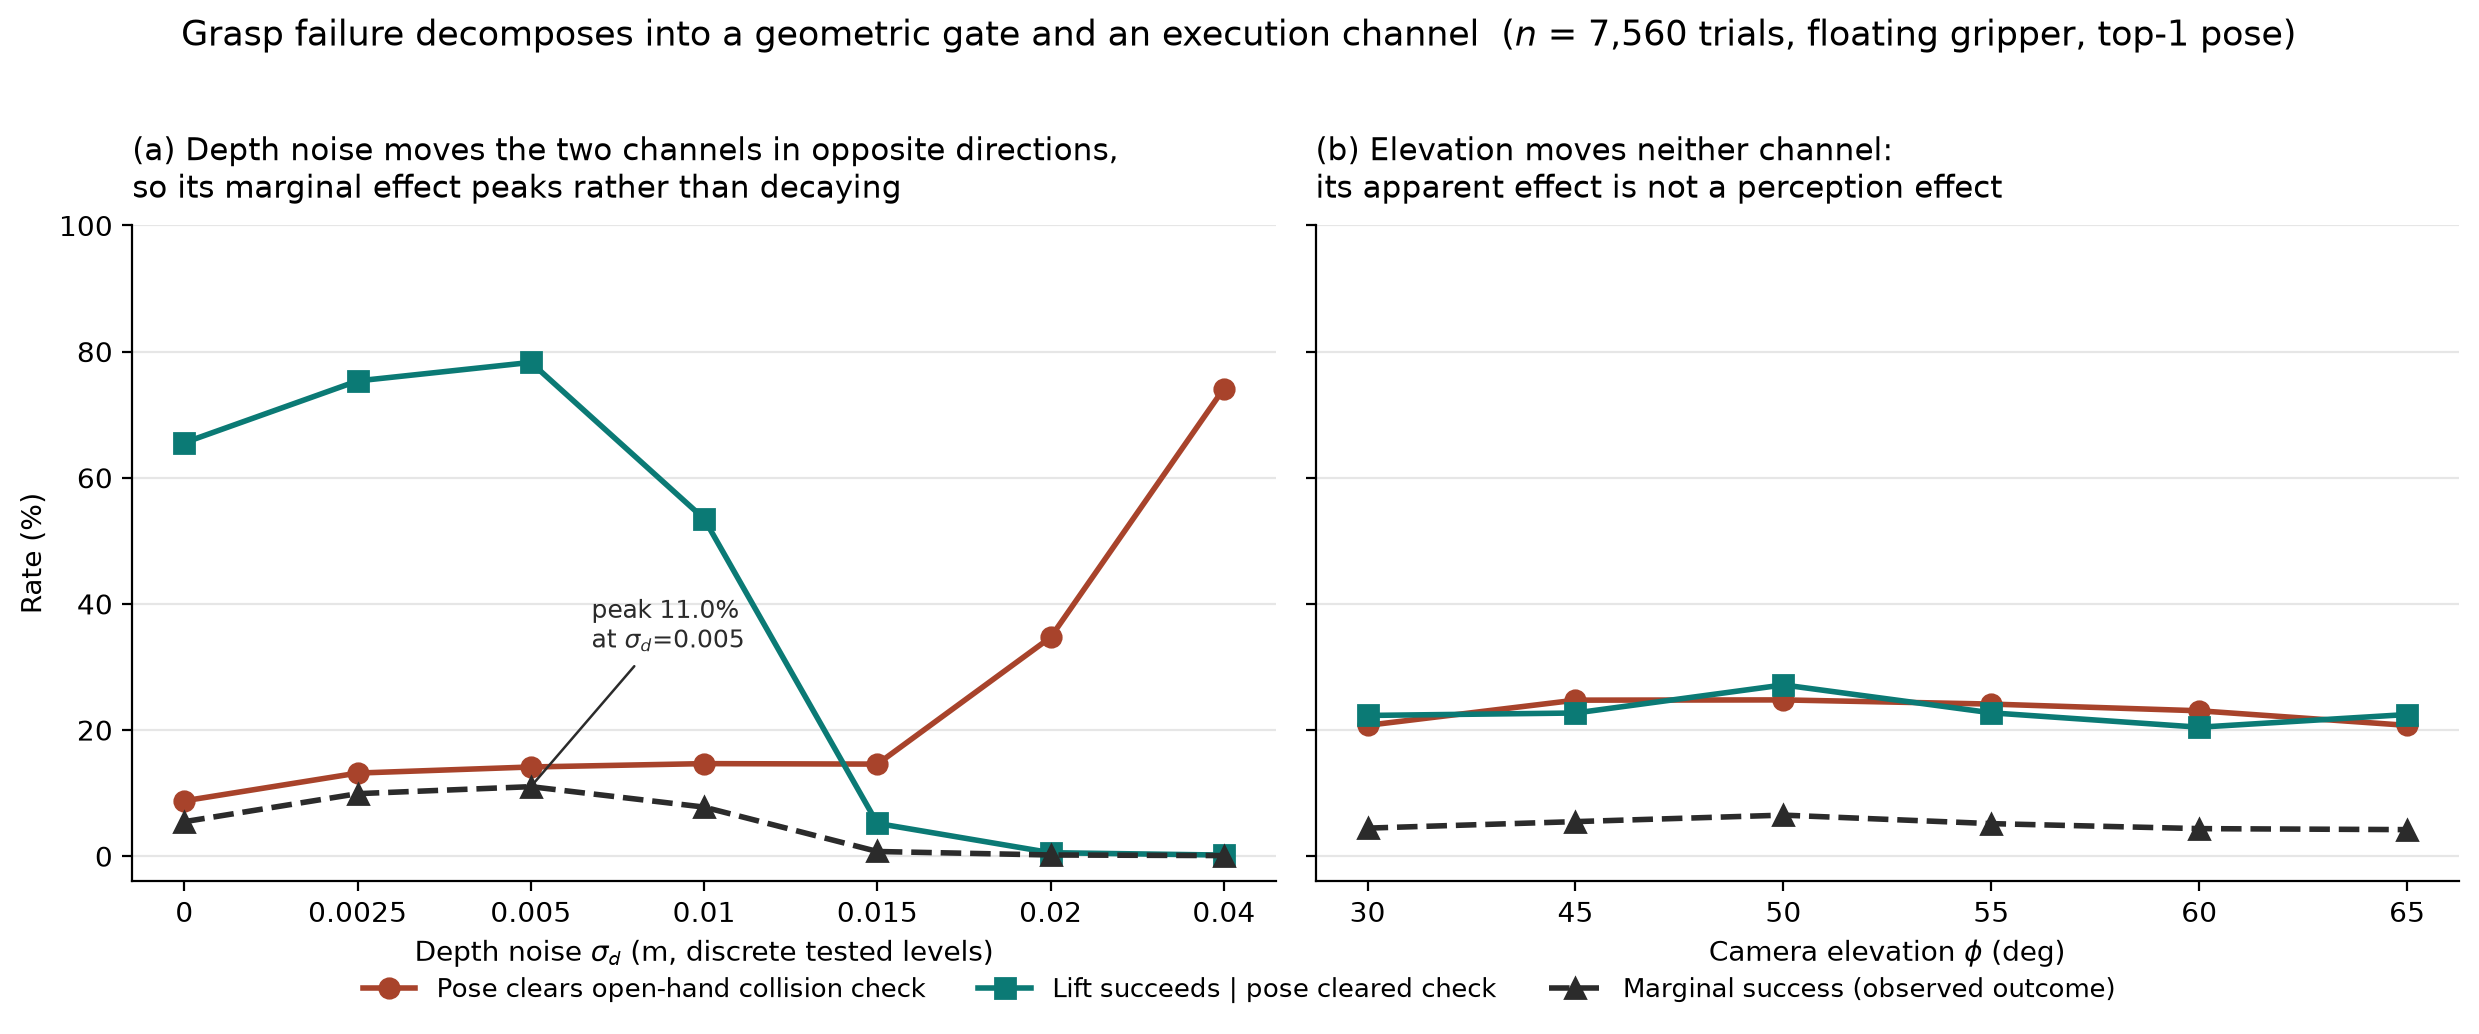
\includegraphics[width=\textwidth]{results/figures/gate_decomposition.png}
  \caption[Gate and execution channel decomposition]{Decomposition of grasp outcome into the geometric gate and the execution channel. (a) Depth noise raises the gate-pass rate while destroying post-gate success, so the observed marginal rate peaks at $\sigma_d = 0.005$ rather than decaying monotonically. (b) Camera elevation moves neither channel appreciably, so its small marginal variation is not a perception effect.}
  \label{fig:gate_decomposition}
\end{figure}

Because the two factors move in opposition, the marginal success rate is non-monotone: it \emph{rises} from 5.5\% at $\sigma_d = 0$ to a peak of 11.0\% at $\sigma_d = 0.005$ before collapsing. Read from the marginal rate alone, the data appear to say that mild depth noise improves grasping. The decomposition shows that this is an artefact of composition rather than a physical benefit: pose quality is degrading monotonically throughout, while the geometric gate is simultaneously becoming easier to pass for the same reason.

Figure~\ref{fig:failure_modes} shows the same phenomenon as a change in the composition of failures. As $\sigma_d$ increases, pre-grasp collision is progressively replaced by execution failures in which the gripper closes without securing the object. The dominant failure mode is effectively converted into its opposite: at low noise poses fail by sitting too close to the object, and at high noise they fail by sitting too far from it.

\begin{figure}[t]
  \centering
  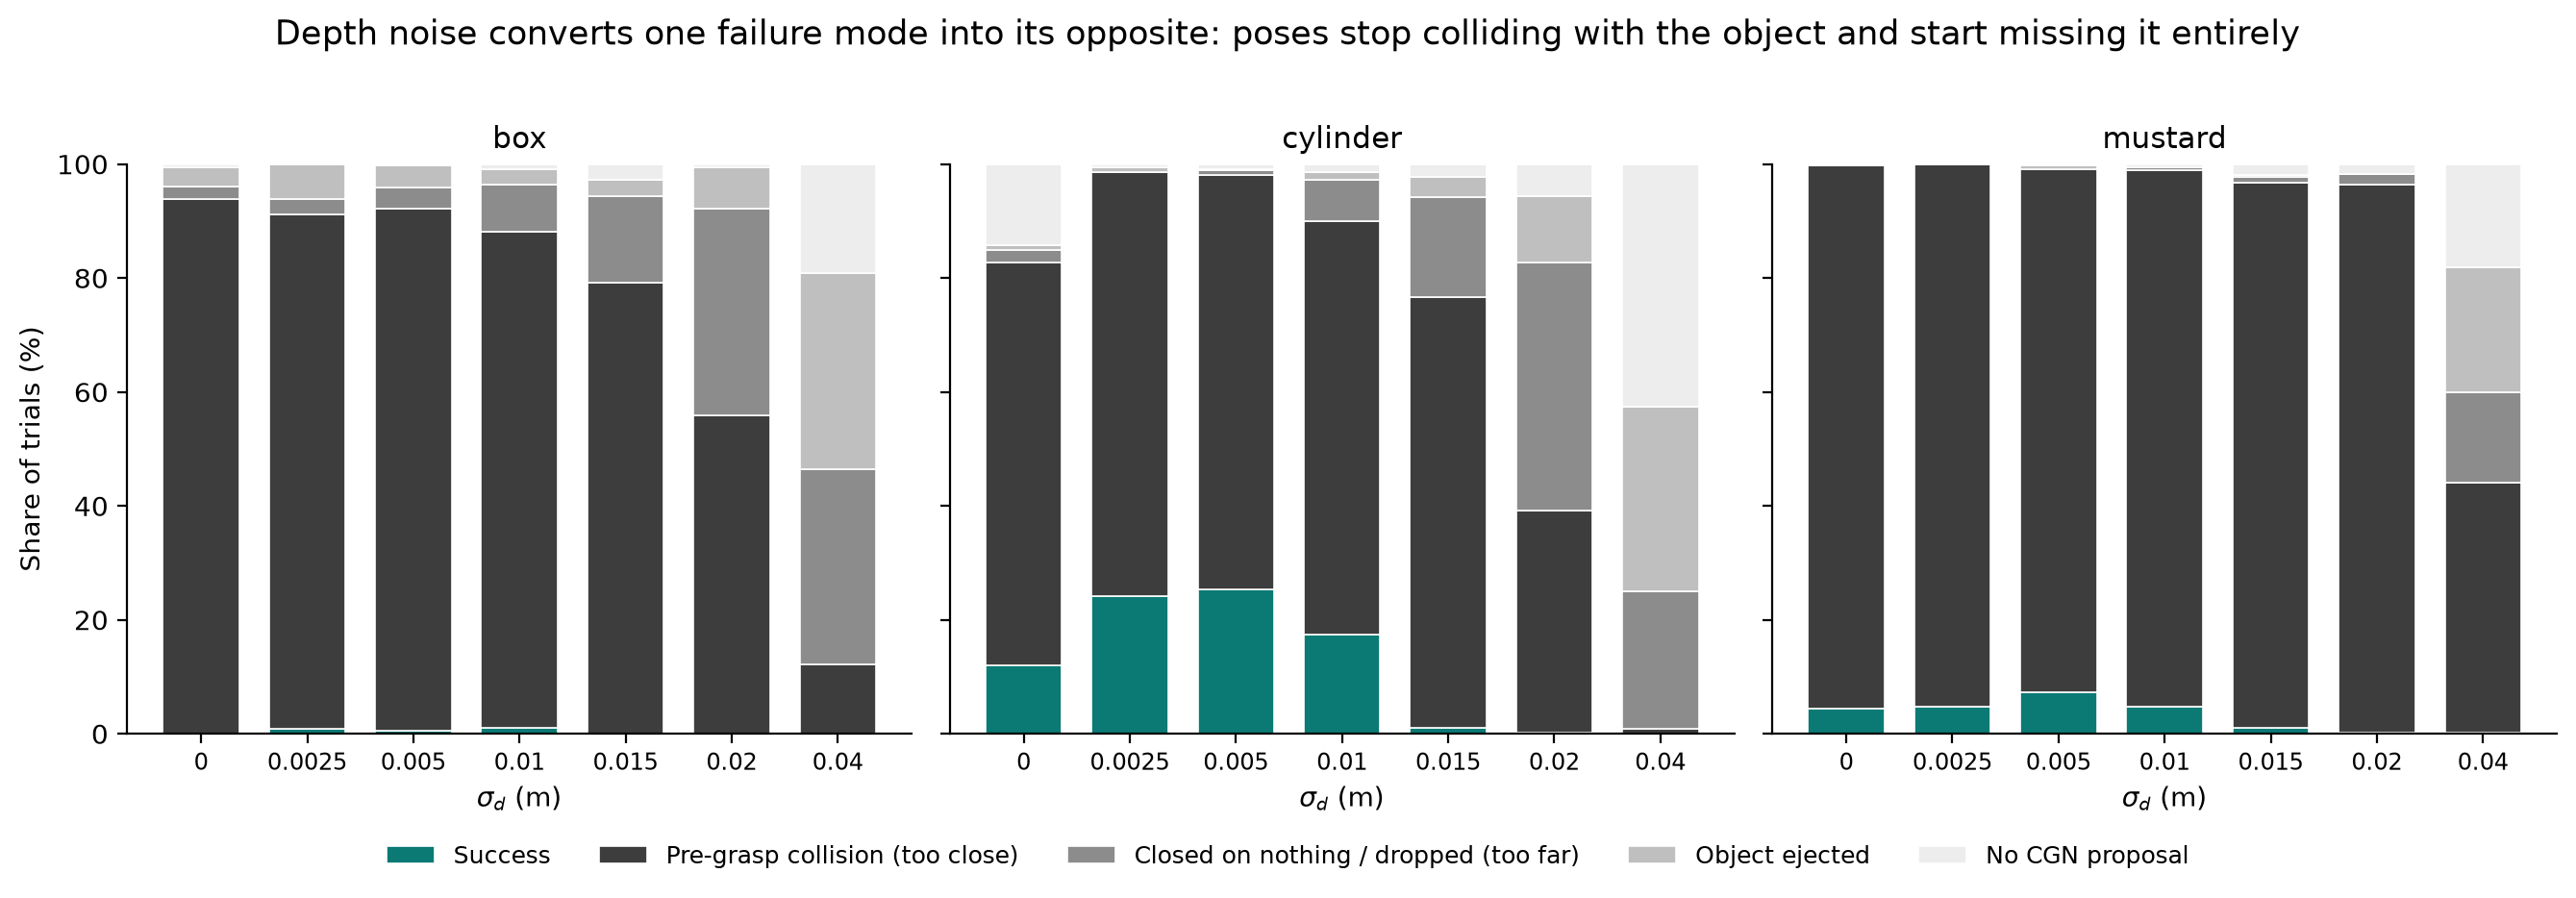
\includegraphics[width=\textwidth]{results/figures/failure_modes_v2.png}
  \caption[Failure-mode composition against depth noise]{Composition of terminal outcomes against depth noise, by object. Increasing $\sigma_d$ trades pre-grasp collision for execution failure, and the balance between the two differs sharply across geometries.}
  \label{fig:failure_modes}
\end{figure}

This tension is structural rather than incidental. The open-hand collision check rejects poses for being too close to the object, while the grasp objective requires poses that are close enough to enclose it. The two criteria are in partial opposition, and any perturbation that displaces the pose distribution outward will relieve one at the expense of the other.

\subsection{Intermediate Variables}

Table~\ref{tab:intermediates} reports the mediating variables among candidate-producing trials. Point cloud completeness $C_{pc}$ is flat across $\sigma_d$ by construction, since the segmentation mask is rendered before noise injection. The number of candidates falls steeply, from 49.2 at $\sigma_d = 0$ to 5.3 at $\sigma_d = 0.04$, and grasp confidence declines after $\sigma_d = 0.005$.

\begin{table}[t]
  \caption{Mediating variables by depth noise, among trials that produced at least one candidate.}
  \label{tab:intermediates}
  \centering
  \begin{tabular}{lrrrrr}
    \toprule
    $\sigma_d$ (m) & $n$ & $\bar{C}_{pc}$ & $\bar{q}_{\text{grasp}}$ & $\bar{e}_{\text{pose}}$ (m) & $\bar{n}_{\text{grasps}}$ \\
    \midrule
    0.0000 & 1026 & 0.0162 & 0.237 & 0.075 & 49.2 \\
    0.0025 & 1078 & 0.0161 & 0.260 & 0.067 & 44.1 \\
    0.0050 & 1075 & 0.0161 & 0.266 & 0.065 & 38.5 \\
    0.0100 & 1070 & 0.0161 & 0.266 & 0.058 & 37.0 \\
    0.0150 & 1055 & 0.0161 & 0.254 & 0.049 & 28.6 \\
    0.0200 & 1052 & 0.0162 & 0.248 & 0.048 & 16.9 \\
    0.0400 &  793 & 0.0166 & 0.210 & 0.061 &  5.3 \\
    \bottomrule
  \end{tabular}
\end{table}

Mean pose error $e_{\text{pose}}$ also \emph{falls} with noise over most of the range, from 0.075\,m to 0.048\,m. This is a selection effect and is analysed in Section~\ref{sec:reversals}.

\section{Viewpoint and Sparsity Act on Neither Channel}
\label{sec:viewpoint_sparsity}

Table~\ref{tab:decomp_view} reports the same decomposition for elevation, azimuth, and retention fraction. Elevation is the clearest negative result in the study: across a 35° range the gate-pass rate varies only between 20.7\% and 24.8\%, and post-gate success only between 20.4\% and 27.2\%. Its sole systematic trace is a mild decline in whether Contact-GraspNet returns anything at all, from 96.0\% at $\phi = 30°$ to 90.3\% at $\phi = 65°$. Retention fraction behaves similarly, with post-gate success confined to 21.2--24.5\% across a fourfold change in point density.

Azimuth is the one viewpoint variable with a consistent effect, and it acts on the execution channel: post-gate success falls monotonically from 28.3\% at $\theta = 0°$ to 17.4\% at $\theta = 90°$ while the gate-pass rate stays flat at roughly 23\%.

\begin{table}[t]
  \caption{Stage-wise decomposition by camera elevation, azimuth, and retention fraction.}
  \label{tab:decomp_view}
  \centering
  \begin{tabular}{llrrrrr}
    \toprule
    \textbf{Variable} & \textbf{Level} & $n$ & \textbf{Proposal (\%)} & \textbf{Gate pass (\%)} & \textbf{Success $\mid$ gate (\%)} & \textbf{Marginal (\%)} \\
    \midrule
    \multirow{6}{*}{$\phi$ (deg)}
      & 30 & 1260 & 96.0 & 20.7 & 22.3 & 4.4 \\
      & 45 & 1260 & 97.5 & 24.7 & 22.7 & 5.5 \\
      & 50 & 1260 & 96.7 & 24.8 & 27.2 & 6.5 \\
      & 55 & 1260 & 94.1 & 24.1 & 22.7 & 5.2 \\
      & 60 & 1260 & 92.6 & 23.1 & 20.4 & 4.4 \\
      & 65 & 1260 & 90.3 & 20.7 & 22.5 & 4.2 \\
    \midrule
    \multirow{3}{*}{$\theta$ (deg)}
      &  0 & 2520 & 94.5 & 23.8 & 28.3 & 6.4 \\
      & 45 & 2520 & 94.7 & 22.9 & 23.1 & 5.0 \\
      & 90 & 2520 & 94.4 & 22.4 & 17.4 & 3.7 \\
    \midrule
    \multirow{4}{*}{$\rho$}
      & 0.25 & 1890 & 89.9 & 24.7 & 23.6 & 5.2 \\
      & 0.50 & 1890 & 95.7 & 24.1 & 24.5 & 5.7 \\
      & 0.75 & 1890 & 96.7 & 20.7 & 21.2 & 4.2 \\
      & 1.00 & 1890 & 96.0 & 22.9 & 22.7 & 5.0 \\
    \bottomrule
  \end{tabular}
\end{table}

\section{Object Geometry Dominates the Execution Channel}
\label{sec:geometry}

The largest effect in the study is not a perceptual variable at all. Table~\ref{tab:decomp_object} shows that post-gate success is 1.5\% for the box, against 35.4\% for the cylinder and 35.0\% for the mustard bottle: a factor of more than twenty between geometries, compared with the roughly 1.4-fold spread produced by any viewpoint variable. The box is close to ungraspable under this gripper and protocol, and its 0.4\% marginal success rate is what drags the pooled figure down.

The two channels also separate by object in an informative way. The mustard bottle has by far the lowest gate-pass rate (9.6\%), reflecting an irregular surface that leaves few collision-free approach poses, but the poses that do clear the gate are as good as the cylinder's. The box shows the opposite pattern: poses clear the gate at an ordinary rate (24.5\%) and then almost never hold.

\begin{table}[t]
  \caption{Stage-wise decomposition by object. Each row aggregates 2{,}520 trials.}
  \label{tab:decomp_object}
  \centering
  \begin{tabular}{lrrrr}
    \toprule
    \textbf{Object} & \textbf{Proposal (\%)} & \textbf{Gate pass (\%)} & \textbf{Success $\mid$ gate (\%)} & \textbf{Marginal (\%)} \\
    \midrule
    Box (sugar)     & 96.5 & 24.5 &  1.5 &  0.4 \\
    Cylinder        & 90.4 & 35.9 & 35.4 & 11.5 \\
    Mustard bottle  & 96.7 &  9.6 & 35.0 &  3.3 \\
    \bottomrule
  \end{tabular}
\end{table}

Geometry also moderates the noise effect rather than merely shifting it. Table~\ref{tab:object_by_sigma} shows that the cylinder and mustard bottle both start near-perfect at low noise and collapse, but at different rates: the cylinder is already at 5.0\% by $\sigma_d = 0.015$ while the mustard bottle retains 44.4\%. The box never exceeds 9.1\% at any noise level. This is the interaction that preliminary marking anticipated, and it answers the question directly: the causal structure is not consistent across geometry.

\begin{table}[t]
  \caption{Post-gate success rate (\%) by object and depth noise, with the number of gate-passing trials in each cell in parentheses.}
  \label{tab:object_by_sigma}
  \centering
  \begin{tabular}{lrrrrrrr}
    \toprule
    & \multicolumn{7}{c}{$\sigma_d$ (m)} \\
    \cmidrule(lr){2-8}
    \textbf{Object} & 0.0000 & 0.0025 & 0.0050 & 0.0100 & 0.0150 & 0.0200 & 0.0400 \\
    \midrule
    Box (sugar)     &   0.0 (20) &   8.6 (35) &  6.9 (29) &  9.1 (44) &  0.0 (65) &  0.0 (157) & 0.0 (247) \\
    Cylinder        &  79.6 (54) &  96.7 (90) & 95.8 (95) & 67.0 (94) &  5.0 (80) &  0.5 (200) & 0.0 (204) \\
    Mustard bottle  & 100.0 (16) & 100.0 (17) & 92.9 (28) & 89.5 (19) & 44.4~~(9) & 12.5~~~(8) & 0.7 (137) \\
    \bottomrule
  \end{tabular}
\end{table}

\section{Two Associational Reversals}
\label{sec:reversals}

The dataset contains two places where the marginal association points in the opposite direction to the within-stratum relationship. Both are dissolved by conditioning on the structure, and together they form the empirical case for the mechanistic audit.

The first is the non-monotone noise effect of Section~\ref{sec:noise_channels}. Marginally, moving from a noise-free sensor to $\sigma_d = 0.005$ doubles the success rate. Conditional on clearing the gate, the same move is neutral-to-mildly-positive, and beyond it the effect is catastrophic; the apparent benefit comes almost entirely from the gate-pass rate rising from 8.8\% to 14.1\%.

The second concerns the pose-error mediator. Among gate-passing trials the raw correlation between $e_{\text{pose}}$ and success is \emph{positive} for two of three objects ($+0.09$ for the box, $+0.25$ for the cylinder, $-0.15$ for the mustard bottle), which would suggest that worse localisation helps. Within every noise stratum the relationship has the expected sign: at $\sigma_d = 0$ successful trials average $e_{\text{pose}} = 0.083$\,m against 0.119\,m for failures, at $\sigma_d = 0.0025$ it is 0.075\,m against 0.110\,m, and at $\sigma_d = 0.005$ it is 0.073\,m against 0.094\,m. The reversal arises because $\sigma_d$ lowers $e_{\text{pose}}$ and destroys success simultaneously, so pooling across noise levels inverts the sign.

Neither reversal is exotic; both are ordinary confounding. The point is that both are present in the observable outcome data that a diagnostic system would receive, and both would lead an associational diagnostician to a conclusion of the wrong sign. A pre-registered structural model that knows the pipeline's stage order avoids both without having to discover them.

\section{Top-$k$ Collision Filtering as an Intervention on the Gate}
\label{sec:topk}

Section~\ref{sec:decomposition} shows that the gate is where most trials are lost. Contact-GraspNet practice normally addresses this by considering more than the top-ranked proposal, so we ran a targeted intervention: at a single favourable viewpoint ($\phi = 55°$, $\theta = 45°$, $\sigma_d = 0$, $\rho = 1.0$) with the cylinder, candidates were rejected in rank order until a collision-free pose was found, up to $k = 20$. Across 100 trials this protocol reaches 89\% success, and every one of the 11 failures is a trial in which no collision-free pose was found within the top 20.

The same 100 trials also record which rank was executed. Top-1 would have succeeded on only those trials whose selected rank was 0, so the comparison in Table~\ref{tab:topk_ablation} does not mix viewpoint, object, or scoring rule.

\begin{table}[t]
  \caption{Same 100 clean cylinder trials ($\phi=55°$, $\theta=45°$, $\sigma_d=0$, $\rho=1$, clamp-and-lift). Top-1 is read off \texttt{selected\_rank} on the filtered run, not a second batch.}
  \label{tab:topk_ablation}
  \centering
  \begin{tabular}{lrr}
    \toprule
    \textbf{Protocol} & \textbf{Success} & \textbf{Pre-grasp collision} \\
    \midrule
    Top-1 only (no retry) & 22/100 (22\%) & 78\% \\
    Top-20 + collision filter & 89/100 (89\%) & 11\% \\
    \bottomrule
  \end{tabular}
\end{table}

Top-$k$ therefore rescued 67 of the 100 trials that top-1 would have lost to collision; the mean selected rank among successes is 3.13. The remaining 11\% are trials in which every candidate in the top 20 still intersected the object.

Two comparisons put this in context. The matched cell in the main study, which executes the top-ranked pose only, succeeded in 2 of 5 trials; pooled over all viewpoints at $\sigma_d = 0$ and $\rho = 1.0$, the cylinder's success rate under top-1 selection is 10.0\% with a gate-pass rate of 11.1\%. The intervention therefore removes most of the gate loss and confirms that the low headline rate of Section~\ref{sec:descriptive} is dominated by pose selection rather than by perception or execution.

Three caveats apply. The favourable viewpoint was chosen after inspecting the main grid, so the 89\% figure characterises the protocol's ceiling rather than an expected operating rate. The filtered protocol uses the lighter clamp-and-lift criterion rather than the full shake disturbance used in the main study, so part of the gap is criterion rather than selection. And within this cell success coincides exactly with clearing the gate, which means the filtered configuration carries no execution-channel information; it is a boundary case in which the outcome is determined entirely by pose availability, and it is therefore not a suitable basis for fitting the SCM.

\section{Pilot Diagnostic Results (Proximity Outcome)}
\label{sec:scm_fit}

The confirmatory causal claim of this chapter is the three-stage decomposition, not a re-fit of the parametric SCM on physical $Y$. The numbers below are a method demonstration on the 426-trial proximity analysis sample (432 trials minus six WinError rows). They must not be read as physical-grasp effects: $Y$ under that criterion is a near-deterministic function of $e_{\text{pose}}$. A re-fit on the 7{,}560-trial grid would also need a gate node, which is absent from the pre-registered graph (Section~\ref{sec:decomposition}).

Table~\ref{tab:scm_fit} records the pilot fit. $C_{pc}$ is almost entirely viewpoint geometry ($R^2 = 0.893$); $\sigma_d$ and $\rho$ are excluded by construction because the segmentation mask is rendered before noise and downsampling. The hurdle separates the two degradations: $\sigma_d$ dominates whether any proposal appears (AUC~$= 0.943$), while $\rho$ dominates how many appear given that the gate is cleared. Among surviving trials, $q_{\text{grasp}}$ has $R^2 = 0.699$ with a positive $\log(n_{\text{grasps}})$ term (order-statistic selection). An earlier $e_{\text{pose}}$ specification that treated $q_{\text{grasp}}$ as a mediator was falsified by the dataflow audit (Assumption~4, Section~\ref{sec:falsification}): the two quantities are siblings sharing an $\arg\max$ index. Full coefficients are in \texttt{results/scm\_coefficients.csv}.

\begin{table}[t]
  \caption{Pilot SCM fit on the 426-trial proximity sample. Not a confirmatory physical-grasp result.}
  \label{tab:scm_fit}
  \centering
  \begin{tabular}{llrrl}
    \toprule
    \textbf{Eq.} & \textbf{Outcome} & \textbf{$R^2$ / pseudo-$R^2$} & \textbf{$n$} & \textbf{Notes} \\
    \midrule
    Eq.~1 & $C_{pc}$       & 0.893 & 426 & OLS; HC3 SE \\
    Eq.~2A & $\text{has\_grasps}$ & 0.554 & 426 & Logistic; AUC = 0.943 \\
    Eq.~2B & $n_{\text{grasps}}$  & ---   & 285 & NegBin; conditional on has\_grasps=1 \\
    Eq.~3  & $q_{\text{grasp}}$  & 0.699 & 285 & OLS; HC3 SE \\
    Eq.~4  & $e_{\text{pose}}$   & 0.625 & 285 & OLS; HC3 SE \\
    \bottomrule
  \end{tabular}
\end{table}

Paired single-variable resets on the same pilot failures produced \texttt{results/counterfactual\_groundtruth.csv}: of 292 failures, 167 (57.2\%) have no single-variable fix under a full clean-baseline reset. That figure is a ground-truth re-simulation on the proximity outcome, not an SCM prediction, and it is irreducibility \emph{within the intervention magnitude tested} (Section~\ref{sec:limitations}).

The LLM baseline was scored on that same ground truth (Table~\ref{tab:attribution}). On 95 single-variable-fixable trials it reaches 31.6\% mean accuracy, uneven across variables ($\sigma_d$ 55.6\%, $\phi$ 43.5\%, $\theta$ 0/35, $\rho$ 0/1). On all 292 trials, including joint and irreducible cases, accuracy is 10.3\%, below the 57.2\% majority-class baseline of always predicting \texttt{none}. Scoring Algorithm~\ref{alg:diagnosis} against the same file was not closed, so Hypotheses~\ref{hyp:comparison} and~\ref{hyp:accuracy} are not evaluated. Hypothesis~\ref{hyp:consistency} is supported only in the weak sense that the SCM is deterministic given fixed inputs, while the LLM's mean agreement across three $T{=}1.0$ queries is 78.1\% on 292 trials (Table~\ref{tab:consistency}).

\begin{table}[t]
  \caption{Pilot attribution accuracy (\%) on 95 single-variable-fixable proximity trials (Tier~1). SCM row not scored.}
  \label{tab:attribution}
  \centering
  \begin{tabular}{lccccr}
    \toprule
    \textbf{Method}
      & $\sigma_d$ ($n{=}36$) & $\rho$ ($n{=}1$) & $\phi$ ($n{=}23$) & $\theta$ ($n{=}35$) & \textbf{Mean} ($n{=}95$) \\
    \midrule
    Causal SCM (ours) & \multicolumn{5}{c}{\itshape not scored against ground truth} \\
    LLM baseline (T1) & 55.6 & 0.0 & 43.5 & 0.0 & 31.6 \\
    \bottomrule
  \end{tabular}
\end{table}

\begin{table}[t]
  \caption{Pilot attribution consistency (agreement across 3 queries at $T{=}1.0$), 95 single-cause proximity trials, Tier~1.}
  \label{tab:consistency}
  \centering
  \begin{tabular}{lcccc}
    \toprule
    & $\sigma_d$ & $\rho$ & $\phi$ & $\theta$ \\
    \midrule
    LLM baseline agreement rate & 78.7\% & 100.0\%$^\dagger$ & 78.3\% & 74.3\% \\
    Causal SCM (ours) & \multicolumn{4}{c}{100\% (deterministic)} \\
    \bottomrule
  \end{tabular}
\end{table}

$^\dagger$The $\rho$ column has $n=1$. SCM determinism is a structural property, not an empirical accuracy result.


% ============================================================
%  CHAPTER 7: DISCUSSION
% ============================================================
\chapter{Discussion}
\label{ch:discussion}

The confirmatory result is not a monotone noise--success curve. It is a decomposition: most of the 7{,}560-trial grid is lost at the open-hand gate (72.8\% pre-grasp collision; 5.0\% success), depth noise moves the gate and the execution channel in opposite directions, and object geometry dominates post-gate hold. That is the mechanistic audit the thesis set out to run. The 432-trial proximity study remains in the record as the pilot that motivated the redesign and hosted the SCM-fit and LLM comparison; those numbers are not physical-grasp effects.

\section{What the Confirmatory Grid Shows}
\label{sec:observations}

Unfiltered top-1 execution on a physically scored floating gripper does not reproduce laboratory Contact-GraspNet headlines. The 5.0\% pooled rate is mostly pose selection: among trials that produce candidates, only 23.1\% clear the gate, and of those only 23.1\% hold through the shake. The residual execution-channel failure (roughly three quarters of gate-passing trials) is what shows that physical $Y$ is not a relabelling of the collision check.

Depth noise is not a single mechanism. Gate-pass rises from 8.8\% at $\sigma_d = 0$ to 74.1\% at $\sigma_d = 0.04$ while success given the gate falls from 65.6\% to 0.2\%. The marginal rate therefore peaks at 11.0\% under mild noise---an associational reversal that would lead a diagnostician who sees only $Y$ to conclude that a little noise helps. Conditioning on the stage order dissolves it. The same pattern appears as a sign flip on $e_{\text{pose}}$ when noise strata are pooled (Section~\ref{sec:reversals}).

Geometry vs.\ perception is not a residual caveat; it is the largest effect. Post-gate success is 1.5\% for the sugar box against $\approx$35\% for the cylinder and mustard bottle. Perception still matters---the cylinder and mustard collapse at different $\sigma_d$---but a pooled SCM that ignores shape would average two different mechanisms.

The filtered arm isolates the gate. At one post-hoc clean viewpoint, top-$k$ collision rejection ($k=20$) reaches 89\% under clamp-and-lift, with every remaining failure a residual collision. On the same 100 trials, top-1 would have succeeded in only 22\% (Table~\ref{tab:topk_ablation}). The matched unfiltered cell is 2/5; cylinder top-1 across clean viewpoints is 10.0\%. The 89\% figure is a ceiling, not an operating rate, and it uses a lighter criterion than the main-grid shake. It does show that the headline 5.0\% is dominated by executing the top-ranked colliding pose, not by an inability of the weld-hand to lift a geometrically valid grasp.

Full-arm inverse kinematics is not a discarded curiosity. The first stack reached the commanded $(x,y)$ to about a millimetre and still failed to lift, for gripper-geometry reasons unrelated to perception. A later 6-DoF due-diligence pass reached collision-filtered Contact-GraspNet poses in 25/25 clean cylinder trials and still recorded 0/25 frictional lifts. A lift exists, but only under the listed contact compromises of Appendix~\ref{sec:arm_v4}. That is why the confirmatory bed isolates pose quality. The 432-trial proximity rule was the interim stand-in after the first abandonment; it is circular with respect to $e_{\text{pose}}$ and is not the outcome of Sections~\ref{sec:descriptive}--\ref{sec:topk}.

\section{Pilot Diagnostics, Not Headline Comparison}
\label{sec:pilot_diagnostics}

On the proximity sample the surrogate fit is strong where the dataflow is simple ($C_{pc}$ $R^2 = 0.893$; has\_grasps AUC~$= 0.943$) and the hurdle splits $\sigma_d$ (any proposal) from $\rho$ (how many). That is useful as a method check. It is not a model of physical $Y$, and it omits the collision gate that dominates the confirmatory grid. Re-fitting Equations~\eqref{eq:cpc}--\eqref{eq:ep} without that node would recover the wrong sign on the marginal $\sigma_d \to Y$ association (Section~\ref{sec:reversals}).

The LLM baseline (31.6\% on 95 single-cause proximity trials; 10.3\% on 292) shows that text-only associative diagnosis is weak and internally noisy (78.1\% agreement). Algorithm~\ref{alg:diagnosis} was not scored against \texttt{results/counterfactual\_groundtruth.csv}, so Hypotheses~\ref{hyp:comparison} and~\ref{hyp:accuracy} are unevaluated. Hypothesis~\ref{hyp:consistency} is supported only as a structural contrast (deterministic SCM vs.\ stochastic LLM), not as an accuracy ranking. The SCM/LLM gap is a secondary illustration of what encoding the pipeline buys; it is not the thesis's central claim, and it is not claimed on physical grasps.

The 57.2\% (167/292) irreducible-failure rate is a ground-truth re-simulation on the proximity outcome under full clean-baseline resets, concentrated at $\phi = 60°$. Contribution~4 is that rate with those qualifications, not a floating-gripper quantity.

\section{Assumptions and Limitations}
\label{sec:limitations}

\begin{enumerate}
  \item \textbf{Expert-specified graph, missing the gate.} The DAG is pre-registered from dataflow, not discovered. Yang and Bareinboim~\cite{yang2025hierarchy} show that $\mathcal{L}_3$ queries require assumptions no $\mathcal{L}_1$ or $\mathcal{L}_2$ dataset can fully falsify. The confirmatory grid adds a further misspecification: the open-hand collision gate is a mediator on the path to physical $Y$ and is not a node in Figure~\ref{fig:causal_dag}.

  \item \textbf{Floating-gripper idealisation.} The test assumes the end-effector can be held at any commanded pose. Unreachable or self-colliding proposals for the full manipulator are not penalised. Success rates are not full-system pick rates. Open-hand teleport to the final pose is an ACRONYM-style validity check and may be slightly pessimistic relative to an approach along the grasp axis. Full-arm due diligence later showed that reach can be solved (25/25 at one clean cell) while frictional lift on those Contact-GraspNet poses remains 0/25 unless forearm collisions are ghosted, geometry is thinned, friction is raised, and---for a held lift---a weld is latched (Appendix~\ref{sec:arm_v4}).

  \item \textbf{Fixed disturbance and contact parameters.} Lift height, jitter, the 40\%-of-lift threshold, the $\pm$70\,N per-finger cap, and friction-5.0 pads were chosen once on physical grounds, not swept. Quoted rates are conditional on that profile. The pads are elevated relative to rubber-on-plastic to compensate for box-fingertip area.

  \item \textbf{Two scoring rules on the filtered arm.} The 89\% cell uses clamp-and-lift; the 7{,}560-trial grid uses shake. They are not interchangeable.

  \item \textbf{Gaussian noise.} Additive i.i.d.\ depth noise omits structured Kinect-class artefacts (IR dropout, discontinuity bias, multipath).

  \item \textbf{Simulation only; diagnosis only.} No sim-to-real claim. Recovery actions are out of scope.

  \item \textbf{Pilot outcome for parametric SCM and LLM.} Fit statistics, LLM accuracy, and the 57.2\% irreducibility figure use $Y = \mathbf{1}\{e_{\text{pose}} < D_\tau\}$. Under that rule $Y$ and $e_{\text{pose}}$ are nearly the same quantity. Six WinError rows (1.4\%) affect only that sample.

  \item \textbf{Intervention magnitude (pilot).} Every counterfactual reset is a full return to the clean baseline, not a partial correction, and $\phi_{\text{nom}} = 45°$ is itself a choice. The 57.2\% rate is irreducibility within that operationalisation. The SCM's $\Delta_v$ ranking was not scored against the same ground truth; the $\phi = 30°$ CGN bias is a known surrogate misspecification that would be amplified by abduction.

  \item \textbf{Attribution vs.\ actual causation.} Algorithm~\ref{alg:diagnosis} uses $\arg\max_v \Delta_v$. Halpern--Pearl minimality~\cite{halpern2005causes} is not checked.
\end{enumerate}

\section{Future Work}
\label{sec:future_work}

\begin{itemize}
  \item \textbf{Re-fit the SCM on the floating-gripper grid, with the gate.} Add $G$ as a mediator, condition execution-channel equations on $G=1$, and only then score Algorithm~\ref{alg:diagnosis} against paired counterfactuals under physical $Y$. Until that is done, Hypotheses~\ref{hyp:accuracy} and~\ref{hyp:comparison} remain open.

  \item \textbf{Intervention-magnitude sensitivity.} Repeat the paired resets at intermediate values (e.g.\ $\sigma_d \in \{0, 0.01, 0.02\}$), on physical $Y$, to test whether irreducibility is robust or an artefact of full clean-baseline resets.

  \item \textbf{Partial-observability abduction.} Hide $(\sigma_d, \rho, \phi, \theta)$ from the diagnostician and infer them from intermediates, so abduction is not bookkeeping.

  \item \textbf{VLM baseline with images.} The present LLM is text-only by design. Supplying the rendered view would test whether structural knowledge still adds anything once the baseline can see the scene.

  \item \textbf{Non-linear equations and NPSEM-ie residuals.} Splines or a small network for the $\phi = 30°$ CGN bias; pairwise residual correlations across equations as a check on independent exogenous noise.

  \item \textbf{Real-robot validation and closed-loop recovery.} Controlled physical perturbations; use the diagnosis to choose a camera move or a filter rather than stopping at attribution.
\end{itemize}


% ============================================================
%  CHAPTER 8: CONCLUSION
% ============================================================
\chapter{Conclusion}
\label{ch:conclusion}

This thesis asked whether a pre-registered mechanistic SCM, built from the known dataflow of a grasp pipeline, can audit why a grasp failed when the experimenter controls the perturbation. The confirmatory experimental bed is a weld-constrained floating-gripper hold/lift test on 7{,}560 factorial trials across three objects. Physical success is 5.0\%. Most of that loss is the open-hand collision gate (72.8\%), not a missing Contact-GraspNet proposal (5.4\%). Depth noise raises gate-pass while destroying post-gate hold, so the marginal rate is non-monotone. Object geometry dominates execution. Filtering collisions at one clean viewpoint lifts clamp-and-lift success to 89\%, which shows that the unfiltered 5.0\% is a pose-selection figure, not a proof that the gripper cannot lift.

Two earlier stacks are reported because they were run, not because they are the result. Full-arm inverse kinematics reached the commanded position on the first attempt and still failed to lift; a later 6-DoF pass reached Contact-GraspNet poses in 25/25 clean trials with 0/25 frictional lifts, and produced a held lift only under the contact compromises of Appendix~\ref{sec:arm_v4}. The 432-trial proximity study then scored $Y$ as a threshold on $e_{\text{pose}}$: useful as a pilot---it showed a strong noise gradient (70.4\% to 0.0\% under that rule) and hosted the SCM fit, the paired counterfactual ground truth (57.2\% irreducible under full resets), and the LLM baseline (31.6\% on single-cause trials)---but circular as a physical-grasp outcome. Counterfactual attribution on the SCM was implemented as a procedure; it was not scored against that ground truth, and it was not re-fit on physical $Y$.

The engineering path (first IK, then proximity, then mocap, then a weld-constrained floating hand, with a later full-arm due-diligence return) is a sequential debugging chain, documented in Appendix~\ref{app:implementation}. The causal argument does not depend on Contact-GraspNet specifically: any grasp model and any simulator that yields depth, a pose, and an independent physical outcome can host the same audit, provided the outcome is not a function of a mediator already in the graph.


% ============================================================
%  BIBLIOGRAPHY
% ============================================================
\begin{thebibliography}{99}

\bibitem{bohg2014data}
J.~Bohg, A.~Morales, T.~Asfour, and D.~Kragic,
``Data-Driven Grasp Synthesis---A Survey,''
\emph{IEEE Trans.\ Robot.}, vol.~30, no.~2, pp.~289--309, 2014.

\bibitem{sundermeyer2021contact}
M.~Sundermeyer et al., ``Contact-GraspNet: Efficient 6-DoF Grasp
Generation in Cluttered Scenes,'' \emph{IEEE ICRA}, 2021,
pp.~13438--13444.

\bibitem{fang2020graspnet}
H.-S.~Fang et al., ``GraspNet-1Billion: A Large-Scale Benchmark for
General Object Grasping,'' \emph{IEEE/CVF CVPR}, 2020,
pp.~11444--11453.

\bibitem{khoshelham2011accuracy}
K.~Khoshelham and S.~O.~Elberink,
``Accuracy and Resolution of Kinect Depth Data for Indoor Mapping
Applications,''
\emph{Sensors}, vol.~12, no.~2, pp.~1437--1454, 2012.

\bibitem{nguyen2012modeling}
C.~V.~Nguyen, S.~Izadi, and D.~Lovell,
``Modeling Kinect Sensor Noise for Improved 3D Reconstruction and
Tracking,'' \emph{IEEE 3DIM/3DPVT}, 2012, pp.~524--530.

\bibitem{murali2020grasp}
A.~Murali et al., ``6-DOF Grasping for Target-Driven Object
Manipulation in Clutter,'' \emph{IEEE ICRA}, 2020, pp.~6232--6238.

\bibitem{hsiao2010contact}
K.~Hsiao et al., ``Contact-Reactive Grasping of Objects with Partial
Shape Information,'' \emph{IEEE/RSJ IROS}, 2010, pp.~1228--1235.

\bibitem{park2018multimodal}
D.~Park et al., ``Multimodal Anomaly Detection for Object-Level
Failure Identification in Manipulation Tasks,''
\emph{IEEE Robot.\ Automat.\ Lett.}, vol.~3, no.~3,
pp.~1991--1998, 2018.

\bibitem{diehl2022whydidifail}
M.~Diehl and K.~Ramirez-Amaro, ``Why Did I Fail? A Causal-Based
Method to Find Explanations for Robot Failures,''
\emph{IEEE Robot.\ Automat.\ Lett.}, vol.~7, no.~4,
pp.~8925--8932, 2022.

\bibitem{ahmed2021causalworld}
O.~Ahmed, F.~Tr\"{a}uble, A.~Goyal, A.~Neitz, M.~W\"{u}thrich,
Y.~Bengio, B.~Sch\"{o}lkopf, and S.~Bauer, ``CausalWorld: A Robotic
Manipulation Benchmark for Causal Structure and Transfer Learning,''
\emph{Int.\ Conf.\ Learn.\ Represent.\ (ICLR)}, 2021.

\bibitem{levine2018learning}
S.~Levine et al., ``Learning Hand-Eye Coordination for Robotic
Grasping with Deep Learning and Large-Scale Data Collection,''
\emph{Int.\ J.\ Robot.\ Res.}, vol.~37, no.~4--5,
pp.~421--436, 2018.

\bibitem{kalashnikov2018scalable}
D.~Kalashnikov et al., ``Scalable Deep Reinforcement Learning for
Vision-Based Robotic Manipulation,'' \emph{CoRL}, 2018,
pp.~651--673.

\bibitem{ahn2022saycan}
M.~Ahn et al., ``Do As I Can, Not As I Say: Grounding Language in
Robotic Affordances,'' \emph{arXiv:2204.01691}, 2022.

\bibitem{driess2023palm}
D.~Driess et al., ``PaLM-E: An Embodied Multimodal Language Model,''
\emph{arXiv:2303.03378}, 2023.

\bibitem{pearl2009causality}
J.~Pearl, \emph{Causality: Models, Reasoning, and Inference},
2nd~ed.\ Cambridge Univ.\ Press, 2009.

\bibitem{pearl2018book}
J.~Pearl and D.~Mackenzie, \emph{The Book of Why: The New Science
of Cause and Effect}. Basic Books, 2018.

\bibitem{todorov2012mujoco}
E.~Todorov, T.~Erez, and Y.~Tassa,
``MuJoCo: A Physics Engine for Model-Based Control,''
\emph{IEEE/RSJ IROS}, 2012, pp.~5026--5033.

\bibitem{calandra2018more}
R.~Calandra et al., ``More Than a Feeling: Learning to Grasp and
Regrasp Using Vision and Touch,''
\emph{IEEE Robot.\ Automat.\ Lett.}, vol.~3, no.~4,
pp.~3300--3307, 2018.

\bibitem{liu2026activevla}
Z.~Liu, Y.~Gu, Y.~Wang, X.~Xue, and Y.~Fu,
``ActiveVLA: Injecting Active Perception into Vision-Language-Action
Models for Precise 3D Robotic Manipulation,''
\emph{IEEE/CVF Conf.\ Comput.\ Vis.\ Pattern Recognit.\ (CVPR)}, 2026.

\bibitem{liang2023code}
J.~Liang et al., ``Code as Policies: Language Model Programs for
Embodied Control,'' \emph{IEEE ICRA}, 2023, pp.~9493--9500.

\bibitem{huang2023voxposer}
W.~Huang et al., ``VoxPoser: Composable 3D Value Maps for Robotic
Manipulation with Language Models,'' \emph{CoRL}, 2023.

\bibitem{nakamura1986inverse}
Y.~Nakamura and H.~Hanafusa, ``Inverse Kinematics Solutions with
Singularity Robustness for Robot Manipulator Control,''
\emph{ASME J.\ Dyn.\ Syst.\ Meas.\ Control}, vol.~108, no.~3,
pp.~163--171, 1986.

\bibitem{menagerie2022}
MuJoCo Menagerie Contributors, ``MuJoCo Menagerie: A Collection of
Physically Accurate Robot Models,''
\url{https://github.com/google-deepmind/mujoco_menagerie}, 2022.

\bibitem{corke2017robotics}
P.~Corke, \emph{Robotics, Vision and Control: Fundamental Algorithms
in MATLAB}, 2nd~ed.\ Springer, 2017.

\bibitem{siciliano2009robotics}
B.~Siciliano, L.~Sciavicco, L.~Villani, and G.~Oriolo,
\emph{Robotics: Modelling, Planning and Control}. Springer, 2009.

\bibitem{chiaverini1997singularity}
S.~Chiaverini, ``Singularity-Robust Task-Priority Redundancy Resolution
for Real-Time Kinematic Control of Robot Manipulators,''
\emph{IEEE Trans.\ Robot.\ Automat.}, vol.~13, no.~3,
pp.~398--410, 1997.

\bibitem{qi2017pointnetpp}
C.~R.~Qi, L.~Yi, H.~Su, and L.~J.~Guibas,
``PointNet++: Deep Hierarchical Feature Learning on Point Sets in a
Metric Space,''
\emph{Advances in Neural Information Processing Systems (NeurIPS)},
vol.~30, 2017.

\bibitem{yang2025hierarchy}
H.~Yang and E.~Bareinboim,
``A Hierarchy of Graphical Models for Counterfactual Inferences,''
\emph{Advances in Neural Information Processing Systems (NeurIPS)}, 2025.

\bibitem{cartwright1989}
N.~Cartwright,
\emph{Nature's Capacities and Their Measurement},
Clarendon Press, Oxford, 1989.

\bibitem{halpern2005causes}
J.~Y.~Halpern and J.~Pearl,
``Causes and Explanations: A Structural-Model Approach---Part I: Causes,''
\emph{British Journal for the Philosophy of Science}, vol.~56, no.~4,
pp.~843--887, 2005.

\bibitem{vonk2023disentangling}
M.~C.~Vonk, N.~Malekovic, T.~B\"ack, and A.~V.~Kononova,
``Disentangling Causality: Assumptions in Causal Discovery and Inference,''
\emph{Artificial Intelligence Review}, vol.~56, pp.~10613--10649, 2023.

\bibitem{richardsonrobins2013}
T.~S.~Richardson and J.~M.~Robins,
``Single World Intervention Graphs (SWIGs): A Unification of the
Counterfactual and Graphical Approaches to Causality,''
Center for Statistics and the Social Sciences, University of Washington,
Working Paper No.~128, 2013.

\bibitem{rubenstein2017consistency}
P.~K.~Rubenstein, S.~Weichwald, S.~Bongers, J.~M.~Mooij, D.~Janzing,
M.~Grosse-Wentrup, and B.~Sch\"olkopf,
``Causal Consistency of Structural Equation Models,''
\emph{Proc.\ 33rd Conference on Uncertainty in Artificial Intelligence
(UAI)}, 2017.

\bibitem{yang2026hierarchy,
  title={A hierarchy of graphical models for counterfactual inferences},
  author={Yang, Hongshuo and Bareinboim, Elias},
  booktitle={Advances in Neural Information Processing Systems},
  volume={38},
  pages={130941--130988},
  year={2026}
}

\end{thebibliography}

% ============================================================
%  APPENDICES
% ============================================================
\appendix

% ============================================================
%  APPENDIX: IMPLEMENTATION AND DEVELOPMENT
% ============================================================
\chapter{Implementation and Development}
\label{app:implementation}

This appendix documents the implementation process in detail, including the construction of the simulation environment, the iterative development of the control pipeline, and the critical bugs that were encountered and resolved. The goal is to provide an honest account of the engineering challenges involved in building a working simulation-to-inference pipeline, as these challenges significantly influenced the final experimental design.

\section{Simulation Environment Construction}
\label{sec:sim_construction}

\subsection{The Mesh Unavailability Problem}

The Franka Emika Panda arm model available in MuJoCo Menagerie~\cite{menagerie2022} is the standard reference model for simulation research involving this robot. However, the Menagerie distribution uses Git Large File Storage~(LFS) for the detailed mesh assets (\texttt{.stl} files) that define the visual and collision geometry of each link. In the development environment used for this project, Git LFS was not available, which meant that the mesh files could not be downloaded. Attempting to load the Menagerie \texttt{panda.xml} without the mesh files resulted in an immediate parsing error from MuJoCo.

This necessitated a complete reconstruction of the Panda arm using MuJoCo's built-in primitive shapes: capsules, boxes, and cylinders. The kinematic chain---the positions, orientations, and axis definitions of all seven revolute joints---was transcribed exactly from the Menagerie \texttt{panda.xml}. The inertial properties (mass, centre of mass, and diagonal inertia tensors) for each link were also preserved exactly. Only the visual and collision geometry was changed: each link's detailed mesh was replaced by one or two capsule primitives with dimensions chosen to approximately envelop the real link geometry.

\subsection{Scene Structure}

The resulting scene file (\texttt{grasp\_scene\_v2.xml}) contains the following elements:

\begin{enumerate}
  \item \textbf{Ground plane and table.} A flat ground plane and a table modelled as a box body at position $(0.5, 0, 0.2)$\,m with half-extents $(0.3, 0.4, 0.2)$\,m, giving a 40\,cm-tall table surface.

  \item \textbf{Target object.} A cylinder (radius 0.036\,m, half-height 0.055\,m) placed at $(0.5, 0, 0.455)$\,m, i.e., on top of the table with its centre 5.5\,cm above the table surface. The cylinder is connected to the world via a free joint, giving it 6 degrees of freedom for translation and rotation. The mass is set to 0.05\,kg (light enough for the simplified gripper to support) with high friction ($\mu = 2.5$).

  \item \textbf{Panda arm.} Seven revolute joints (\texttt{joint1}--\texttt{joint7}) with the exact DH-compatible positions and orientations from the Menagerie model. Each joint has armature (0.1) and damping (1.0) parameters. The hand body is positioned at $z = 0.107$\,m above the flange with a $22.5°$ yaw offset (implemented as a quaternion rotation). Two prismatic finger joints slide along the hand's local $Y$-axis with range $[0, 0.04]$\,m.

  \item \textbf{Actuators.} Seven position-controlled actuators for the arm joints, implemented as MuJoCo ``general'' actuators with gains and biases matching the Menagerie model (e.g., joint 1: gain = 4500, bias = $[0, -4500, -450]$). An eighth actuator controls the gripper via a tendon coupling the two finger joints, with control range $[0, 255]$ (255 = open, 0 = closed).

  \item \textbf{Perception camera.} A massless body (\texttt{perception\_camera\_body}) at a default position, containing a camera with 45° vertical field of view. The body has a small box geom for visualisation but with \texttt{contype=0} and \texttt{conaffinity=0} so it does not participate in collision detection.

  \item \textbf{Home keyframe.} A keyframe that sets the initial joint configuration to the standard Panda home pose: $[0, 0, 0, -\pi/2, 0, \pi/2, -\pi/4]$ for the arm joints, with fingers fully open (0.04\,m each) and the gripper control set to 255.
\end{enumerate}

The following excerpt shows the key structural elements of the scene XML:

\begin{lstlisting}[style=xml,caption={Excerpt from \texttt{grasp\_scene\_v2.xml} showing the target object and perception camera.},label={lst:scene_xml}]
<!-- Target object (cylinder = cup proxy) -->
<body name="target_object" pos="0.5 0 0.455">
  <freejoint/>
  <inertial pos="0 0 0" mass="0.15"
    diaginertia="0.0002 0.0002 0.0001"/>
  <geom name="cup" type="cylinder" size="0.036 0.055"
    rgba="0.1 0.5 0.8 1" mass="0.05" condim="4"
    friction="2.5 0.01 0.0001"/>
</body>

<!-- Perception camera body -->
<body name="perception_camera_body"
      pos="0.5 -0.7 0.9">
  <camera name="perception_camera" pos="0 0 0"
    fovy="45"/>
  <geom type="box" size="0.02 0.03 0.02"
    rgba="0.2 0.8 0.2 1"
    contype="0" conaffinity="0"/>
</body>
\end{lstlisting}

\subsection{Gripper Geometry: Visual Meshes vs Collision Primitives}
\label{sec:gripper_geometry}

A notable difference exists between the high-fidelity visual representation of the Panda gripper often seen in robotics simulations and the gripper geometry used in this experiment's active physics scene (\texttt{grasp\_scene\_v2.xml}). 

When first loading the Panda arm from MuJoCo Menagerie, the end-effector is typically rendered using complex visual meshes provided by the manufacturer. While visually appealing, these complex non-convex meshes pose significant challenges for physics engines during contact resolution. Calculating penetrations and friction forces between complex meshes and target objects can lead to non-deterministic bouncing, interpenetration, or simulation instability---particularly critical flaws for an automated factorial study requiring precise reproducibility.

To ensure stable, fast, and deterministic contact dynamics, the simulation environment was rebuilt using simplified collision primitives (capsules and boxes) for the robot's links and gripper fingers. This is a standard optimization in reinforcement learning and manipulation research. The confirmatory causal analysis concerns the effect of perception degradation on the proposed 6-DoF grasp pose under the floating-gripper protocol; the simplified collision geometry keeps contact resolution deterministic when that pose is tested. (The inverse-kinematics stack that first motivated primitive fingers is the abandoned execution path of Section~\ref{sec:ik_controller}.)

\subsection{qpos Layout}

A critical implementation detail is the layout of MuJoCo's generalised position vector \texttt{data.qpos}. Because the target object has a free joint that appears before the arm joints in the XML body hierarchy, the \texttt{qpos} array has the following layout (total: $n_q = 16$):

\begin{center}
\begin{tabular}{lll}
\toprule
\textbf{Indices} & \textbf{Count} & \textbf{Description} \\
\midrule
\texttt{qpos[0:3]}  & 3 & Free joint translation $(x, y, z)$ \\
\texttt{qpos[3:7]}  & 4 & Free joint orientation $(q_w, q_x, q_y, q_z)$ \\
\texttt{qpos[7:14]} & 7 & Arm joint angles (joints 1--7) \\
\texttt{qpos[14:16]} & 2 & Finger joint positions \\
\bottomrule
\end{tabular}
\end{center}

Similarly, the velocity vector \texttt{data.qvel} has $n_v = 15$ elements (the free joint contributes 6 velocity DoFs rather than 7 position DoFs because orientation velocity is parameterised as a 3D angular velocity vector rather than a 4D quaternion derivative):

\begin{center}
\begin{tabular}{lll}
\toprule
\textbf{Indices} & \textbf{Count} & \textbf{Description} \\
\midrule
\texttt{qvel[0:3]}  & 3 & Free joint linear velocity \\
\texttt{qvel[3:6]}  & 3 & Free joint angular velocity \\
\texttt{qvel[6:13]} & 7 & Arm joint velocities \\
\texttt{qvel[13:15]} & 2 & Finger joint velocities \\
\bottomrule
\end{tabular}
\end{center}

This distinction between $n_q$ and $n_v$ is important because the Jacobian has $n_v$ columns (one per velocity DoF), not $n_q$. The IK controller must extract columns 6--12 of the Jacobian (corresponding to the arm joint velocities) but write the computed increments to \texttt{qpos[7:14]} (the arm joint positions). Confusing these two index ranges was the source of a critical bug described in Section~\ref{sec:bug_teleportation}.

\section{Critical Bugs Encountered and Resolved}
\label{sec:bugs}

The development process involved several critical bugs that significantly impacted the project timeline. Each bug is described here with its symptoms, root cause, and resolution, to serve as a reference for future work with MuJoCo-based simulation pipelines.

\subsection{Bug 1: Object Teleportation}
\label{sec:bug_teleportation}

\textbf{Symptoms.} During early testing of the IK controller, the target cylinder would spontaneously fly off the table and fall through the floor. The arm joints appeared to remain stationary, and the end-effector did not move toward the target position. The behaviour was completely reproducible across all viewpoints and noise conditions.

\textbf{Root cause.} The IK joint increments were being written to \texttt{qpos[0:7]} instead of \texttt{qpos[7:14]}. This meant that instead of updating the arm joint angles, the controller was modifying the free joint of the target object. The first three elements of \texttt{qpos[0:7]} are the object's $(x, y, z)$ translation, and the next four are its orientation quaternion. The IK increments, which are joint-angle values in radians (typically in the range $[-0.5, 0.5]$), were being interpreted as metre displacements and quaternion components, causing the object to teleport to arbitrary positions.

\textbf{Resolution.} Correcting the index from \texttt{qpos[0:7]} to \texttt{qpos[7:14]} immediately resolved the problem. The arm began moving correctly, and the object remained stationary on the table until contact.

\textbf{Lesson.} MuJoCo's flat \texttt{qpos} array concatenates all joint positions in the order they appear in the body hierarchy. When the scene contains free joints (which contribute 7 elements each), the arm joint indices are offset accordingly. The offset must be determined by careful inspection of the scene XML and the joint ordering.

\subsection{Bug 2: Camera Orientation (Looking Away from Scene)}
\label{sec:bug_camera}

\textbf{Symptoms.} After positioning the camera at the correct spherical coordinates, the rendered depth image showed only the far plane (all pixels at maximum depth). No objects were visible in the image, despite the camera being positioned at a location that should have a clear view of the table and cylinder.

\textbf{Root cause.} The initial camera orientation code used a look-at rotation matrix where the camera's $+Z$ axis pointed toward the target. However, MuJoCo cameras look along $-Z$, not $+Z$. This meant the camera was facing \emph{away} from the scene, pointing into empty space behind its position.

\textbf{Resolution.} The rotation matrix was corrected to use columns $(\hat{\mathbf{r}}, \hat{\mathbf{u}}, -\hat{\mathbf{f}})$ where $\hat{\mathbf{f}}$ is the forward direction toward the target. This places the $-Z$ axis in the forward direction, consistent with MuJoCo's camera convention.

\subsection{Bug 3: Depth Buffer Saturation}
\label{sec:bug_depth}

\textbf{Symptoms.} After fixing the camera orientation, the depth buffer contained values but they were all at or near the far clipping plane value. The rendered depth image appeared uniform, with no discernible structure. Point clouds generated from this depth buffer were either empty or contained only points far from the expected scene geometry.

\textbf{Root cause.} This was a secondary consequence of Bug~2. While the camera orientation had been partially corrected, a sign error in the quaternion conversion resulted in the camera pointing approximately 90° away from the intended direction. The depth buffer was technically valid---it contained the distances to whatever geometry the camera happened to see---but the field of view did not include the target object or table.

\textbf{Resolution.} A complete rewrite of the quaternion conversion code, with explicit unit tests comparing the resulting camera direction against the expected look-at vector, resolved the issue. The quaternion conversion from rotation matrix was implemented using the Shepperd method, which handles all cases (including the degenerate case where the trace of the rotation matrix is negative) robustly.

\subsection{Bug 4: Gripper Contact Problem}
\label{sec:bug_gripper}

\textbf{Symptoms.} When the arm successfully moved to the correct position above the cylinder and the gripper closed, the fingers would close through the object without gripping it. Alternatively, the fingers would stop closing at a gap width larger than the cylinder diameter, failing to make contact.

\textbf{Root cause.} The finger geometry, constructed from primitive box shapes, had dimensions that did not properly match the cylinder radius. The finger inner faces were positioned at $\pm 0.040$\,m from the gripper centre (matching the finger joint range of $[0, 0.04]$\,m), but the cylinder radius was 0.036\,m. When the fingers closed to their minimum separation, the inner surfaces were approximately 0.070\,m apart---wider than the cylinder diameter of 0.072\,m, preventing contact. Additionally, MuJoCo's contact detection requires a minimum overlap (the ``margin'' parameter) of approximately 1\,mm between geom surfaces for a contact to be registered.

\textbf{Resolution.} The finger geometry was adjusted to ensure that the inner faces are positioned at $\pm 0.035$\,m from centre (using box size 0.008\,m with offset 0.005\,m from the joint axis), providing approximately 1\,mm of overlap with the cylinder surface when the fingers are fully closed. The cylinder radius was confirmed at 0.036\,m, and the contact parameters (\texttt{condim=4}, high friction) were tuned to maximise the normal force at contact.

Even with these adjustments, reliable lifting was not achieved across all conditions. The primitive-shape finger geometry lacks the detailed contact surfaces (fingertip pads, serrations) of the real Panda gripper, which are critical for generating the friction forces needed to support the object against gravity. This limitation motivated the adoption of the proximity-based success criterion described in Section~\ref{sec:success_criterion_detail} as an interim, perception-focused outcome. It was not the confirmatory protocol; that is the weld-constrained floating gripper of Section~\ref{sec:from_proximity_to_float}.

\section{From Physical Lift to Proximity Criterion}
\label{sec:lift_to_proximity}

The initial experimental design intended to evaluate grasp success by a physical lift criterion: after the gripper closes, the arm lifts the object vertically, and the trial is successful if the object reaches a height of 0.55\,m (approximately 10\,cm above its resting position). This is the gold standard for grasp evaluation in simulation~\cite{fang2020graspnet}.

In the visual demonstration script (\texttt{demo\_grasp.py}), which runs with the MuJoCo viewer open, individual grasps could sometimes succeed with this criterion: the viewer allowed real-time observation of the contact dynamics, and the grasp parameters (approach speed, gripper closure rate) could be manually tuned for each trial.

However, achieving consistent lift success across 432 headless (no viewer) trials proved impractical, and the underlying reasons all trace back to the same root cause: the primitive-shape gripper cannot reproduce the fine contact mechanics of the real hardware. The fingers have flat box surfaces rather than the real Panda gripper's contoured fingertips, so the contact area is extremely small and the resulting friction force is sensitive to sub-millimetre variations in finger closure. This sensitivity is compounded by the target object itself: the light cylinder (0.05\,kg) is easily displaced by any asymmetric contact force, so if one finger reaches the surface slightly before the other, the object is pushed sideways before the grasp can stabilise, and the tendon actuator---which applies equal force to both fingers regardless of this asymmetry---cannot correct for it. In the visual demonstration script these problems could be caught and corrected by hand, nudging the approach trajectory in real time; the batch experiment, running headless with no per-trial tuning, had no such recourse.

The proximity criterion was adopted as an interim, perception-focused alternative after full-arm lift proved impractical. The thesis's causal claim concerns perception quality and grasp-proposal accuracy, not the robot's ability to physically execute a perfect grasp. Under that interim rule the outcome measured whether the perception-derived grasp position was close enough to the object centroid that, with a competent gripper, contact \emph{would} be established. That rule is circular with respect to $e_{\text{pose}}$ and was retired as the confirmatory outcome once a physically independent test existed.

\section{From Proximity to the Floating-Gripper Protocol}
\label{sec:from_proximity_to_float}

Proximity scoring was never intended as a designed competitor to physical evaluation. After it was in place, execution was rebuilt as a free-floating Panda gripper consuming Contact-GraspNet's full 6-DoF pose (ACRONYM / 6-DoF GraspNet-style). Three implementations were tried in sequence; each was rejected only after a located failure.

A mocap-driven hand teleported the \texttt{hand} body each step. Objects never left the table: mocap bodies contribute no velocity to the contact Jacobian, so friction is never mobilised. A hand-rolled PD force servo on a free body diverged (NaN accelerations) within about 20 steps even in a contact-free hover, so it was rejected without a gain sweep. The adopted mechanism welds a dynamic free-body hand (\texttt{gravcomp="1"}) to an invisible mocap target that is teleported along the trajectory; the Newton solver then couples hand motion through friction. Finger force is capped at $\pm$70\,N per finger; fingertip pads use friction 5.0 to compensate for box-fingertip area. Known-good, known-empty, and known-colliding poses discriminate correctly; genuine Contact-GraspNet proposals lift the cylinder and mustard bottle. Subsidiary fixes retained in the final stack include restoring \texttt{biastype="affine"} on the finger actuator, close-until-first-contact with a bounded squeeze, and a ramped shake to avoid a 2.7\,cm onset impulse.

The confirmatory 7{,}560-trial grid and the filtered top-$k$ check use this weld-hand protocol (Chapter~\ref{ch:method}). The appendix control-loop summary below records the first, abandoned full-arm stack, not that protocol. A later return to the articulated arm is recorded in Section~\ref{sec:arm_v4}.

\section{Full-Arm Due Diligence (v4)}
\label{sec:arm_v4}

After the floating-gripper protocol was in place, a separate 6-DoF stack (\texttt{sim\_arm\_v4.py}, \texttt{run\_arm\_grasp\_v4.py}) was written without modifying the confirmatory pipelines. The aim was due diligence, not a replacement outcome: show whether a Contact-GraspNet pose that the floating gripper can test is reachable by the Panda, and whether frictional lift then follows.

On 25 clean cylinder trials at $\phi=55°$, $\theta=45°$, $\sigma_d=0$, $\rho=1$, with top-$k=20$ open-finger filtering, inverse kinematics reached the selected pose in every trial and the fingers made contact in every trial. Lift success was $0/25$ (mean final lift $<1$\,mm; all \texttt{executed\_dropped}). Fingertip friction in that batch was matched to the floating-gripper pads (sliding coefficient 5). Reach, therefore, is not the missing piece; contact mechanics under the articulated arm still are.

A lift was forced only on a hand-tuned $45°$ diagonal side-grasp of a thinner cylinder ($r=3.0$\,cm rather than $3.6$\,cm), with forearm link collisions ghosted (fingers active), pad and object sliding friction raised to 12, a hard close, and a pre-solved joint-space lift blend. Under those settings, friction produced a $6.8$\,cm peak lift that then slipped (Figure~\ref{fig:arm_v4_friction}). Latching a weld after close held $7.9$\,cm to the top of the trajectory (Figure~\ref{fig:arm_v4_weld}). The weld here is a proof-of-mechanism, not a claim that Menagerie finger contact matches the floating-gripper hold. The listed compromises are why full-arm pick rates are not the confirmatory figure of Chapter~\ref{ch:results}.

\begin{figure}[t]
  \centering
  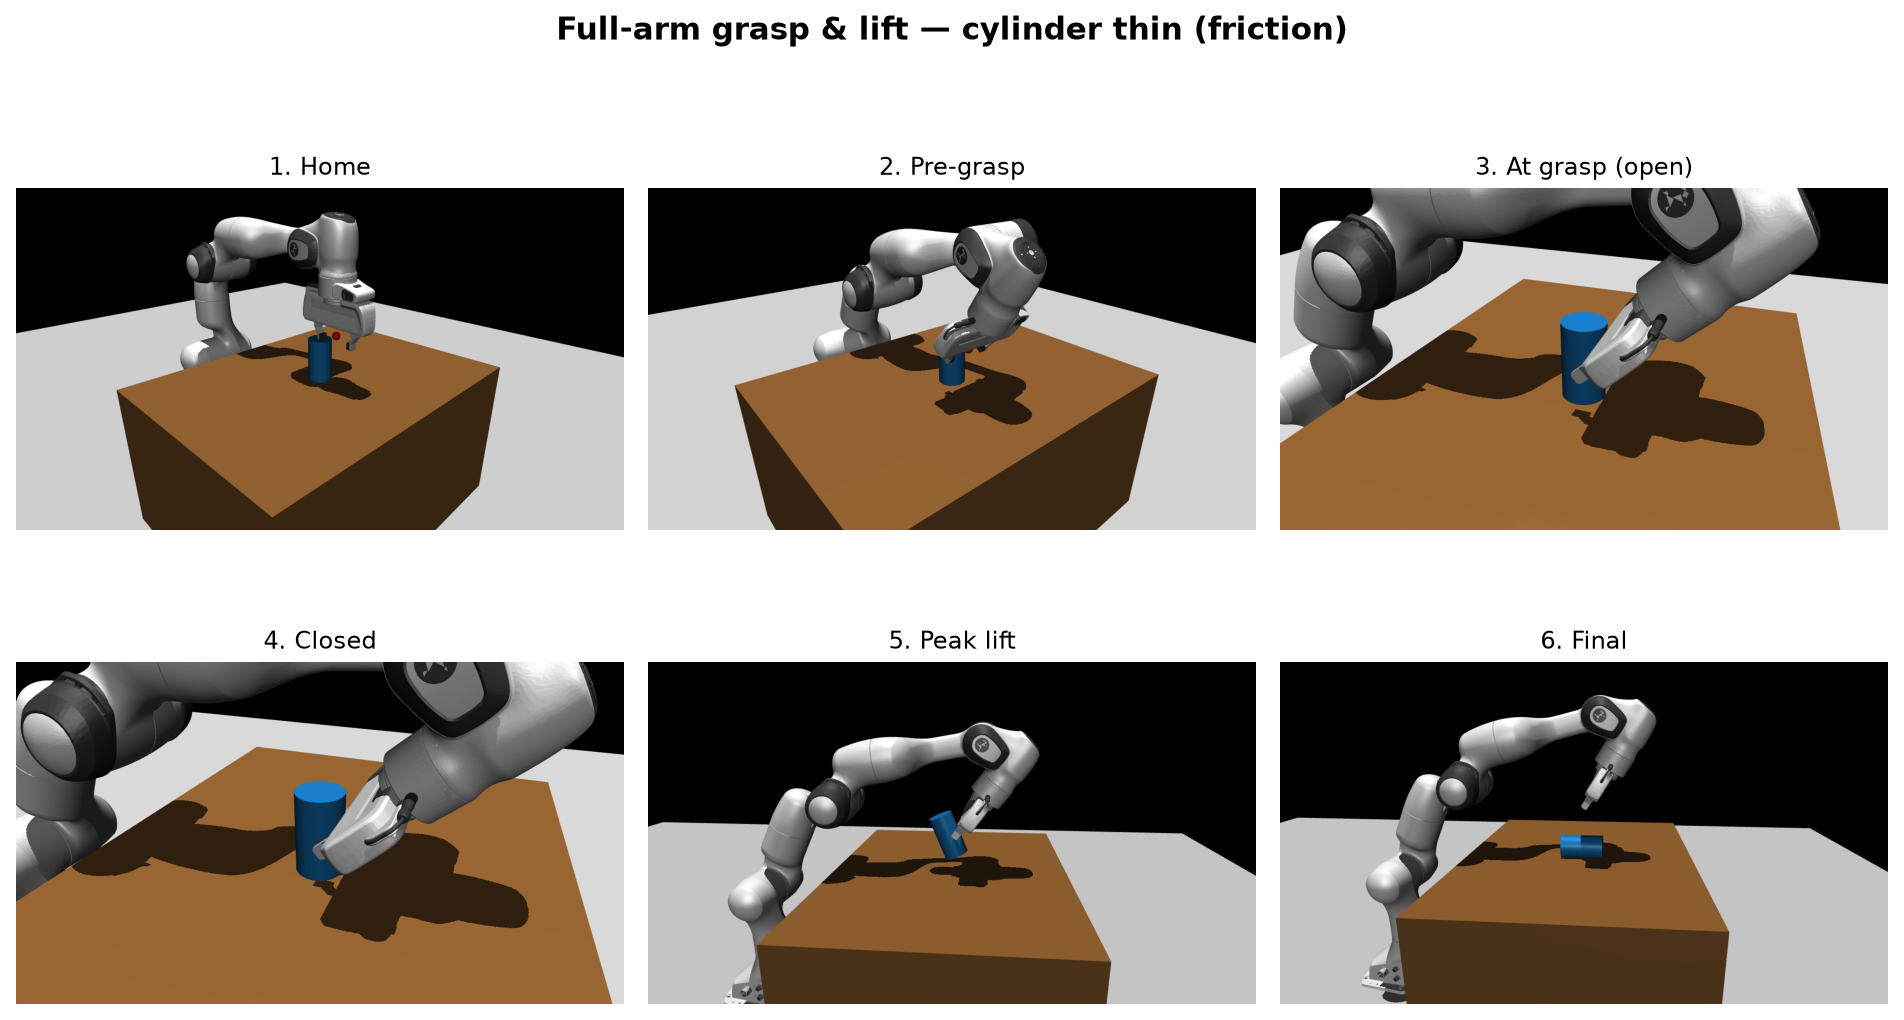
\includegraphics[width=\textwidth]{results/figures/arm_lift_v4/arm_lift_cylinder_thin_friction_stage_panel.png}
  \caption{Full-arm due diligence, friction only: thinner cylinder, diagonal wrist, ghosted forearm collisions, sliding friction 12. The object leaves the table at peak lift and is dropped by the final frame.}
  \label{fig:arm_v4_friction}
\end{figure}

\begin{figure}[t]
  \centering
  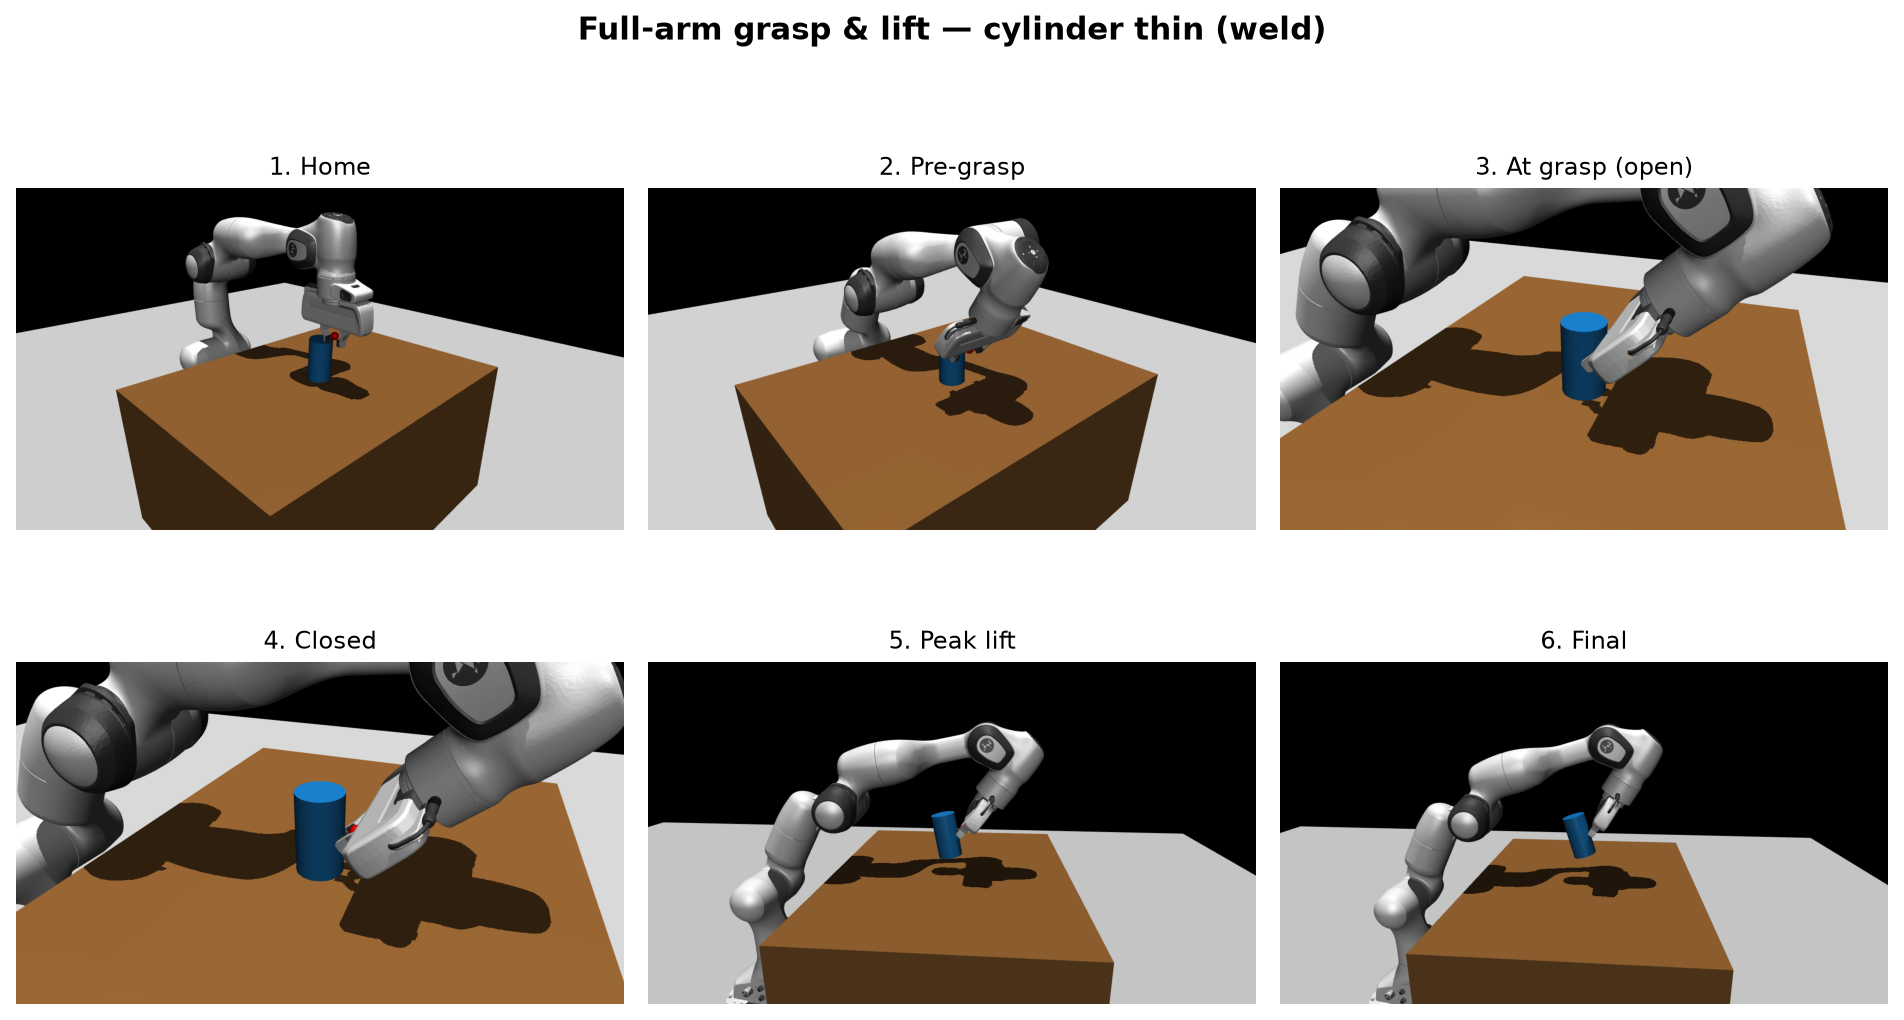
\includegraphics[width=\textwidth]{results/figures/arm_lift_v4/arm_lift_cylinder_thin_weld_stage_panel.png}
  \caption{The same pose with a weld latched after close. The lift is held. This is an explicit scaffolding of contact, not the confirmatory success criterion.}
  \label{fig:arm_v4_weld}
\end{figure}

\section{Automated Control Pipeline Summary}
\label{sec:pipeline_summary}

The following summarises the abandoned full-arm inverse-kinematics stack. The confirmatory protocol is the weld-constrained floating gripper of Section~\ref{sec:from_proximity_to_float}. The v4 due-diligence stack is Section~\ref{sec:arm_v4}.

To clarify the complete chain of causation from perception to motion, this section summarises what exactly moves the arm in the simulation:

\begin{enumerate}
  \item The \textbf{Jacobian DLS} method computes a joint velocity increment $\Delta\mathbf{q} \in \mathbb{R}^7$ from the position error.

  \item The increment is \textbf{scaled and added to} $\texttt{data.qpos[7:14]}$, updating the 7 arm joint angles in MuJoCo's internal state vector.

  \item The updated joint angles are \textbf{mirrored into} $\texttt{data.ctrl[0:7]}$, commanding MuJoCo's position actuators to drive toward the new configuration.

  \item MuJoCo's \textbf{PD actuators generate torques}: the gain term produces a restoring torque proportional to the error between $\texttt{ctrl}$ and the current joint angle, and the bias term provides gravity compensation and damping.

  \item \texttt{mj\_step} \textbf{integrates the equations of motion}, advancing the simulation by one timestep. The joint torques accelerate the links, the positions update, and the arm physically moves.

  \item This process \textbf{repeats} at 500\,Hz (timestep = 0.002\,s) until convergence or timeout.
\end{enumerate}

No human operator intervenes at any stage. The entire process is driven by the Python control script calling MuJoCo functions in a loop.

\section{Perception Pipeline Detail}
\label{sec:perception_pipeline}

The perception pipeline transforms the MuJoCo scene into the input format expected by Contact-GraspNet. The steps are:

\begin{enumerate}
  \item \textbf{Render depth.} MuJoCo's \texttt{Renderer} produces a $480 \times 640$ depth buffer as a NumPy array of float32 values representing distances in metres.

  \item \textbf{Add noise.} Gaussian noise $\mathcal{N}(0, \sigma_d^2)$ is added per-pixel. Values are clipped to $\geq 0$.

  \item \textbf{Render segmentation.} A second render pass produces the segmentation buffer, a $480 \times 640 \times 2$ array where channel 0 contains the geom ID at each pixel. The code iterates over all geoms in the model, identifies those belonging to the target body, and creates a binary mask.

  \item \textbf{Build camera intrinsics.} The $3 \times 3$ intrinsic matrix $\mathbf{K}$ is constructed from the MuJoCo camera's field-of-view parameter (Equation~\ref{eq:focal_from_fov}).

  \item \textbf{Save to NPZ.} The depth, intrinsics, and segmentation are saved to a temporary \texttt{.npz} file, which is loaded by CGN's data loader.

  \item \textbf{CGN point cloud extraction.} CGN's built-in \texttt{extract\_point\_clouds} function back-projects the depth map using the intrinsics matrix and filters points by a z-range $[0.1, 2.0]$\,m.

  \item \textbf{Downsample.} If $\rho < 1.0$, the confirmatory grid retains points by evenly-strided, seed-independent selection (Section~\ref{sec:pointcloud_downsampling}). The 432-trial proximity pilot instead sampled indices uniformly without replacement.

  \item \textbf{CGN inference.} The (possibly downsampled) point cloud is passed to CGN's \texttt{predict\_scene\_grasps}, which returns grasp poses, scores, and contact points.
\end{enumerate}

The following code snippet shows the core perception function:

\begin{lstlisting}[caption={Depth rendering with noise injection and segmentation.},label={lst:render}]
def render_depth_seg(model, data, sigma_d=0.0, rng=None):
    renderer = mujoco.Renderer(model,
                   height=IMG_H, width=IMG_W)
    renderer.enable_depth_rendering()
    renderer.update_scene(data, camera=CAM_NAME)
    depth_raw = renderer.render().copy()
    renderer.disable_depth_rendering()

    renderer.enable_segmentation_rendering()
    renderer.update_scene(data, camera=CAM_NAME)
    seg = renderer.render()
    renderer.close()

    # Binary segmentation: target object = 1
    tgt_bid = mujoco.mj_name2id(model,
        mujoco.mjtObj.mjOBJ_BODY, TARGET_BODY)
    gid_img = seg[:, :, 0]
    seg_map = np.zeros(gid_img.shape, dtype=np.int32)
    for gid in range(model.ngeom):
        if model.geom_bodyid[gid] == tgt_bid:
            seg_map[gid_img == gid] = 1

    # Noise injection (causal variable sigma_d)
    if sigma_d > 0.:
        depth_noisy = np.clip(
            depth_raw + rng.normal(0., sigma_d,
                                   depth_raw.shape),
            0., None).astype(np.float32)
    else:
        depth_noisy = depth_raw.copy()

    return depth_noisy, build_K(model), seg_map
\end{lstlisting}

\section{Software Architecture}
\label{sec:software_architecture}

The codebase is organised into several Python modules:

\begin{itemize}
  \item \texttt{run\_experiments\_v2.py}: Confirmatory batch script. Iterates the 7{,}560-trial floating-gripper grid (3 objects $\times$ 7 $\sigma_d$ $\times$ 4 $\rho$ $\times$ 6 $\phi$ $\times$ 3 $\theta$ $\times$ 5 seeds) and logs physical hold/lift outcomes plus the open-hand collision flag to \texttt{results/experiment\_results\_v2.csv}.

  \item \texttt{run\_experiments\_v3.py}: Filtered top-$k$ collision-rejection arm, used for the clean-cell check of Section~\ref{sec:topk}.

  \item \texttt{run\_experiments.py}: Pilot batch script. Iterates the 432-trial proximity grid ($4 \sigma_d \times 4 \rho \times 3 \phi \times 3 \theta \times 3$ seeds). Not the confirmatory run.

  \item \texttt{sim\_arm\_v4.py} / \texttt{run\_arm\_grasp\_v4.py}: Later full-arm due diligence (6-DoF IK, approach, top-$k$ filter). The 25-trial clean cylinder batch is \texttt{results/experiment\_results\_arm\_v4.csv}. Does not modify the v2/v3 confirmatory scripts.

  \item \texttt{demo\_grasp.py}: A visual demonstration script that opens the MuJoCo viewer and executes a single grasp with real-time visualisation. Useful for debugging and verifying the pipeline visually.

  \item \texttt{mujoco\_cgn\_bridge.py}: A modular bridge between MuJoCo rendering and CGN inference. Contains the rendering, point cloud extraction, CGN inference, and frame transformation functions as a reusable library.

  \item \texttt{grasp\_scene\_v2.xml}: The MuJoCo scene definition file, containing the complete Panda arm model, table, target object, camera, actuators, tendons, and home keyframe.

  \item \texttt{scm\_fit.py}: Fits all five structural equations to the 426-trial proximity analysis sample (pilot diagnostic fit, not a re-fit on physical $Y$).

  \item \texttt{run\_counterfactual\_groundtruth.py}: Re-runs the MuJoCo+CGN simulation for each of the 292 failed \emph{proximity} trials under four single-variable clean-baseline interventions. Outputs \texttt{results/counterfactual\_groundtruth.csv}. Not a floating-gripper re-simulation.
\end{itemize}


\chapter{MuJoCo Scene XML}
\label{app:scene_xml}

The complete scene definition file \texttt{grasp\_scene\_v2.xml} is reproduced below. This file contains the full Panda arm model with primitive-shape geometry, the target object, the perception camera, all actuators and tendons, and the home keyframe.

\begin{lstlisting}[style=xml,caption={Complete scene definition: \texttt{grasp\_scene\_v2.xml}.},label={lst:full_scene}]
<mujoco model="panda_grasp_scene">
  <compiler angle="radian" autolimits="true"
    balanceinertia="true"/>
  <option gravity="0 0 -9.81" timestep="0.002"
    integrator="implicitfast"/>

  <default>
    <geom solref="0.004 1" solimp="0.98 0.99 0.001"/>
  </default>

  <default>
    <default class="panda">
      <joint armature="0.1" damping="1" axis="0 0 1"
        range="-2.8973 2.8973"/>
      <general dyntype="none" biastype="affine"
        ctrlrange="-2.8973 2.8973"
        forcerange="-87 87"/>
      <default class="finger">
        <joint axis="0 1 0" type="slide"
          range="0 0.04"/>
      </default>
    </default>
  </default>

  <worldbody>
    <light pos="0 0 2.5" dir="0 0 -1"
      directional="true"/>
    <geom name="floor" type="plane" size="2 2 0.05"
      rgba="0.85 0.85 0.85 1"/>

    <!-- Table -->
    <body name="table" pos="0.5 0 0.2">
      <geom type="box" size="0.3 0.4 0.2"
        rgba="0.6 0.4 0.2 1"/>
    </body>

    <!-- Target object -->
    <body name="target_object" pos="0.5 0 0.455">
      <freejoint/>
      <inertial pos="0 0 0" mass="0.15"
        diaginertia="0.0002 0.0002 0.0001"/>
      <geom name="cup" type="cylinder"
        size="0.036 0.055"
        rgba="0.1 0.5 0.8 1" mass="0.05"
        condim="4" friction="2.5 0.01 0.0001"/>
    </body>

    <!-- Panda arm: link0 through hand -->
    <!-- (7 revolute joints + 2 finger joints) -->
    <!-- ... (body hierarchy as in main text) ... -->

    <!-- Perception camera -->
    <body name="perception_camera_body"
          pos="0.5 -0.7 0.9">
      <camera name="perception_camera" pos="0 0 0"
        fovy="45"/>
      <geom type="box" size="0.02 0.03 0.02"
        rgba="0.2 0.8 0.2 1"
        contype="0" conaffinity="0"/>
    </body>
  </worldbody>

  <tendon>
    <fixed name="split">
      <joint joint="finger_joint1" coef="0.5"/>
      <joint joint="finger_joint2" coef="0.5"/>
    </fixed>
  </tendon>

  <equality>
    <joint joint1="finger_joint1"
      joint2="finger_joint2"
      solimp="0.95 0.99 0.001" solref="0.005 1"/>
  </equality>

  <actuator>
    <general class="panda" name="actuator1"
      joint="joint1"
      gainprm="4500" biasprm="0 -4500 -450"/>
    <!-- ... actuators 2-7 ... -->
    <general class="panda" name="actuator8"
      tendon="split"
      forcerange="-100 100" ctrlrange="0 255"
      gainprm="0.01568627451 0 0"
      biasprm="0 -100 -10"/>
  </actuator>

  <keyframe>
    <key name="home"
      qpos="0.5 0 0.455 1 0 0 0
        0 0 0 -1.57079 0 1.57079 -0.7853
        0.04 0.04"
      ctrl="0 0 0 -1.57079 0 1.57079
        -0.7853 255"/>
  </keyframe>
</mujoco>
\end{lstlisting}

\chapter{IK Controller Implementation}
\label{app:ik_code}

The complete inverse kinematics controller implementation from \texttt{run\_experiments.py}:

\begin{lstlisting}[caption={Damped Least Squares IK controller.},label={lst:ik_full}]
def ik_move_to(model, data, target_pos,
               max_steps=2000, tol=0.010, lam=0.01):
    """
    Jacobian DLS IK for the 7 Panda arm joints.

    qpos layout (nq=16):
      [0:7]   freejoint of target_object
      [7:14]  arm joints 1-7
      [14:16] finger joints 1-2

    nv layout (nv=15):
      [0:6]   freejoint velocity DOFs
      [6:13]  arm joint velocities 1-7
      [13:15] finger joint velocities
    """
    site_id    = mujoco.mj_name2id(
        model, mujoco.mjtObj.mjOBJ_SITE, EE_SITE)
    jacp       = np.zeros((3, model.nv))
    ARM_QPOS   = slice(7, 14)
    ARM_VEL    = slice(6, 13)
    arm_ranges = model.jnt_range[1:8]

    for _ in range(max_steps):
        mujoco.mj_forward(model, data)
        err = target_pos - data.site_xpos[site_id]
        if np.linalg.norm(err) < tol:
            return True
        mujoco.mj_jacSite(model, data, jacp,
                          None, site_id)
        J  = jacp[:, ARM_VEL]   # (3, 7)
        dq = J.T @ np.linalg.solve(
            J @ J.T + lam * np.eye(3), err)
        sc = min(0.5,
                 0.1 / (np.linalg.norm(dq) + 1e-8))
        data.qpos[ARM_QPOS] += dq * sc
        np.clip(data.qpos[ARM_QPOS],
                arm_ranges[:, 0], arm_ranges[:, 1],
                out=data.qpos[ARM_QPOS])
        data.ctrl[:7] = data.qpos[ARM_QPOS]
        mujoco.mj_step(model, data)
    return False
\end{lstlisting}


\end{document}
